\documentclass[11pt,a5paper,twoside]{book}
\usepackage[T1]{fontenc}
\usepackage[Glenn]{fncychap}
\usepackage{bbm}
\usepackage[font=small]{caption}
\usepackage{amsmath, amsthm, amscd, amsfonts}
\usepackage{mathtools}
\DeclarePairedDelimiter\floor{\lfloor}{\rfloor}
\usepackage{graphicx}
\usepackage{pstricks}
\usepackage{bm}
\usepackage{tabu}
\usepackage[authoryear]{natbib}
\usepackage{multirow}
\usepackage{tocbibind}
\usepackage{cleveref}
\usepackage{resizegather}
\usepackage{textcomp}
\newtheorem{theorem}{Theorem}[chapter]
\newtheorem{lemma}{Lemma}[chapter]
\newtheorem{proposition}{Proposition}[chapter]
\newtheorem{corollary}{Corollary}[chapter]
\newtheorem{property}{Property}[chapter]
\newtheorem{definition}{Definition}[chapter]
\newtheorem{remark}{Remark}[chapter]
\usepackage{numprint}
\newcommand{\HRule}{\rule{\linewidth}{0.5mm}}
\usepackage[
  paperwidth=17cm,
  paperheight=24cm,
  % other options
]{geometry}
%\special{papersize=17cm,24cm}
%
%
%\textwidth=12.5cm
%\textheight=20cm
%\oddsidemargin=0.3cm
%\evensidemargin=-1cm
%\topmargin=-1.5cm

%%%%%%%%%%%%%%%%%%%%%%%%%%%%%%%%%%%%%%%%%%%%%%%%%%%%%%%%%%%%%%%%%
%chapter on new page
%%%%%%%%%%%%%%%%%%%%%%%%%%%%%%%%%%%%%%%%%%%%%%%%%%%%%%%%%%%%%%%%%
\newcommand{\clearemptydoublepage}%
        {\newpage{\pagestyle{empty}\cleardoublepage}}

\renewcommand*\listfigurename{List of figures}
\renewcommand*\listtablename{List of tables}

%\title{Data Splitting and Its Applications}
%\author{Vahid Nassiri}
%	options include 12pt or 11pt or 10pt
%	classes include article, report, book, letter, thesis
\usepackage{setspace}
\usepackage{numprint}
\usepackage{siunitx}
\sisetup{round-mode=places,       % enable rounding
         round-precision=4,       % amounts of digits for rounding
         table-format=-1.4}       % default numeric format
\newcommand\scalemath[2]{\scalebox{#1}{\mbox{\ensuremath{\displaystyle #2}}}}
\usepackage{url}
\usepackage{blindtext}
\usepackage{listings}
\usepackage{afterpage,lscape}
\usepackage{bbm}
\usepackage{amsmath, amsthm, amscd, amsfonts}
\usepackage{graphicx}
\usepackage{pstricks}
%\usepackage[natbib, maxcitenames=3, mincitenames=11, style=apa]{biblatex}
\usepackage{color}
\usepackage{multirow}
\usepackage{tocbibind}

\usepackage{textcomp}
\usepackage{lipsum}
\usepackage{fancyhdr}

\fancyfoot{}
\fancyhead[LE, RO]{\thepage}
\fancyhead[LO]{\leftmark}
\fancyhead[RE]{\rightmark}
%\usepackage{fancyhdr}
\pagestyle{fancy}
%\fancyhf{}
%\renewcommand{\headrulewidth}{0pt}
%\fancyhead[R]{\thepage}
%\fancyhead[RO,LE]{\thepage}
%\fancyhead[LO]{\leftmark}
%\fancyhead[RE]{\rightmark}
\usepackage{afterpage}

\newcommand\blankpage{%
    \null
    \thispagestyle{empty}%
    \addtocounter{page}{-1}%
    \newpage}
\usepackage{amssymb}
\usepackage{fixltx2e}
\usepackage{multirow}
\usepackage{verbatim}
\usepackage[normalem]{ulem}
\usepackage{amsmath}
\usepackage{soul}
\usepackage{color}
\usepackage{epstopdf}% To incorporate .eps illustrations using PDFLaTeX, etc.
\usepackage{subfigure}% Support for small, `sub' figures and tables


\usepackage{kbordermatrix}% http://www.hss.caltech.edu/~kcb/TeX/kbordermatrix.sty
\usepackage{mathtools}
\usepackage{listings}
%\usepackage[a4paper, total={6.5in, 9in},top=37mm]{geometry}
%\usepackage{pgfgantt}
\usepackage{afterpage,lscape}
%\usepackage{bbm}
\usepackage{amsmath, amsthm, amscd, amsfonts}
\usepackage{natbib}
\setcitestyle{authoryear,open={(},close={)}}
%\usepackage{cleveref}
\usepackage{textcomp}
\usepackage{longtable}


\renewcommand{\baselinestretch}{1.4} 
\usepackage[english]{babel}
\usepackage[utf8]{inputenc}
 
\usepackage{pdflscape} % provides the landscape environment
\usepackage{ragged2e} % provides \RaggedLeft
 
\usepackage{fancyhdr}
 
\newcommand{\bftheta}{\mbox{\boldmath $\theta$}}
\newcommand{\BY}{\mbox{\boldmath $Y$}}
\newcommand{\bn}{\mbox{\boldmath $n$}}
\newcommand{\bc}{\mbox{\boldmath $c$}}
  \newcommand{\BZ}{\mbox{\boldmath $Z$}}
 \newcommand{\J}{J\"{o}reskog}
\newcommand{\So}{S\"{o}rbom}
\newcommand{\bcx}{{\bf X}}
\newcommand{\bcy}{{\bf Y}}
\newcommand{\bcz}{{\bf Z}}
\newcommand{\bcu}{{\bf U}}
\newcommand{\bcv}{{\bf V}}
\newcommand{\bfv}{\mbox{\boldmath $v$}}
\newcommand{\bcw}{{\bf W}}
\newcommand{\bci}{{\bf I}}
\newcommand{\bch}{{\bf H}}
\newcommand{\bcb}{{\bf B}}
\newcommand{\bcr}{{\bf R}}
\newcommand{\bcm}{{\bf M}}
\newcommand{\bcf}{{\bf F}}
\newcommand{\bcg}{{\bf G}}
\newcommand{\bcs}{{\bf S}}
\renewcommand{\labelitemii}{$\triangleright$}
\newcommand{\tr}{\mbox{tr}}
\newcommand{\Zik}{\mbox{$Z_i^{(k)}$}}
\newcommand{\bca}{{\bf A}}
\newcommand{\bcd}{{\bf D}}
\newcommand{\bcc}{{\bf C}}
\newcommand{\bce}{{\bf E}}
\newcommand{\ba}{{\bf a}}
\newcommand{\bk}{\mbox{\boldmath{$k$}}}
\newcommand{\bb}{{\bf b}}
\newcommand{\bd}{{\bf d}}
\newcommand{\bx}{{\bf x}}
\newcommand{\by}{{\bf y}}
\newcommand{\bz}{{\bf z}}
\newcommand{\bu}{{\bf u}}
\newcommand{\bv}{{\bf v}}
\newcommand{\bh}{{\bf h}}
\newcommand{\bl}{{\bf l}}
\newcommand{\be}{{\bf e}}
\newcommand{\br}{{\bf r}}
\newcommand{\bw}{{\bf w}}
\newcommand{\bbi}{\bm{b_i}}
\newcommand{\Bb}{\mbox{\boldmath $b$}}
 \newcommand{\BW}{\mbox{\boldmath $W$}}
 \newcommand{\bfbeta}{\mbox{\boldmath $\beta$}}
\newcommand{\de}{\stackrel{D}{=}}
\newcommand{\bt}{\bigtriangleup}
 \newcommand{\BYi}{\mathbf{$\y_i$}}
\newcommand{\bfequiv}{\mbox{\boldmath $\equiv$}}
\newcommand{\bmu}{\mbox{\boldmath $\mu$}}
\newcommand{\bnu}{\mbox{\boldmath $\nu$}}
\newcommand{\bxi}{\mbox{\boldmath $\xi$}}
\newcommand{\btau}{\mbox{\boldmath $\tau$}}
\newcommand{\bgamma}{\mbox{\boldmath $\Gamma$}}
\newcommand{\bphi}{\mbox{\boldmath $\Phi$}}
\newcommand{\bfphi}{\mbox{\boldmath $\varphi$}}
\newcommand{\bfeta}{\mbox{\boldmath $\eta$}}
\newcommand{\bpi}{\mbox{\boldmath $\Pi$}}
\newcommand{\bequiv}{\mbox{\boldmath $\equiv$}}
\newcommand{\bvarepsilon}{\mbox{\boldmath $\varepsilon$}}
\newcommand{\btriangle}{\mbox{\boldmath $\triangle$}}
\newcommand{\bdelta}{\mbox{\boldmath $\Delta$}}
\newcommand{\beps}{\mbox{\boldmath $\epsilon$}}
\newcommand{\btheta}{\mbox{\boldmath $\theta$}}
\newcommand{\balpha}{\mbox{\boldmath $\alpha$}}
\newcommand{\bsphi}{\mbox{\boldmath $\varphi$}}
\newcommand{\bsig}{\mbox{\boldmath $\sigma$}}
\newcommand{\bfpsi}{\mbox{\boldmath $\psi$}}
\newcommand{\bfdelta}{\mbox{\boldmath $\delta$}}
\newcommand{\bsigma}{{\bf \Sigma}}
\newcommand{\bzero}{{\bf 0}}
\newcommand{\bpsi}{\mbox{\boldmath $\Psi$}}
\newcommand{\bep}{\mbox{\boldmath $\epsilon$}}
\newcommand{\bomega}{\mbox{\boldmath $\Omega$}}
\newcommand{\bfomega}{\mbox{\boldmath $\omega$}}
\newcommand{\blambda}{\mbox{\boldmath $\Lambda$}}
\newcommand{\bflambda}{\mbox{\boldmath $\lambda$}}
\newcommand{\bfsigma}{\mbox{\boldmath $\sigma$}}
\newcommand{\bfpi}{{\mbox{\boldmath $\pi$}}}
\newcommand{\bupsilon}{\mbox{\boldmath $\upsilon$}}
\newcommand{\obs}{{\rm obs}}
\newcommand{\mis}{{\rm mis}}
\newcommand{\Xik}{\mbox{$X_i^{(k)}$}}
\newcommand{\Aik}{\mbox{$A_i^{(k)}$}}
\newcommand{\Tik}{\mbox{$T_i^{(k)}$}}
\newcommand{\Qik}{\mbox{$Q_i^{(k)}$}}
 \newcommand{\bfalpha}{\mbox{\boldmath $\alpha$}}
 \newcommand{\bfgamma}{\mbox{\boldmath $\gamma$}}
 \newcommand{\bfSigma}{\mbox{\boldmath $\Sigma$}}
 \newcommand{\bfmu}{\mbox{\boldmath $\mu$}}
  \newcommand{\bfrho}{\mbox{\boldmath $\rho$}}

 \newcommand{\eenvec}{\mbox{\boldmath $1$}}

%%%% from rmarkdown
\usepackage{lmodern}
\usepackage{amssymb,amsmath}
\usepackage{ifxetex,ifluatex}
\usepackage{fixltx2e} % provides \textsubscript
\ifnum 0\ifxetex 1\fi\ifluatex 1\fi=0 % if pdftex
  \usepackage[T1]{fontenc}
  \usepackage[utf8]{inputenc}
\else % if luatex or xelatex
  \ifxetex
    \usepackage{mathspec}
  \else
    \usepackage{fontspec}
  \fi
  \defaultfontfeatures{Ligatures=TeX,Scale=MatchLowercase}
\fi
% use upquote if available, for straight quotes in verbatim environments
\IfFileExists{upquote.sty}{\usepackage{upquote}}{}
% use microtype if available
\IfFileExists{microtype.sty}{%
\usepackage{microtype}
\UseMicrotypeSet[protrusion]{basicmath} % disable protrusion for tt fonts
}{}
\urlstyle{same}  % don't use monospace font for urls
\usepackage{color}
\usepackage{fancyvrb}
\usepackage{cleveref}
\newcommand{\VerbBar}{|}
\newcommand{\VERB}{\Verb[commandchars=\\\{\}]}
\DefineVerbatimEnvironment{Highlighting}{Verbatim}{commandchars=\\\{\}}
% Add ',fontsize=\small' for more characters per line
\usepackage{framed}
\definecolor{shadecolor}{RGB}{248,248,248}
\newenvironment{Shaded}{\begin{snugshade}}{\end{snugshade}}
\newcommand{\AlertTok}[1]{\textcolor[rgb]{0.94,0.16,0.16}{#1}}
\newcommand{\AnnotationTok}[1]{\textcolor[rgb]{0.56,0.35,0.01}{\textbf{\textit{#1}}}}
\newcommand{\AttributeTok}[1]{\textcolor[rgb]{0.77,0.63,0.00}{#1}}
\newcommand{\BaseNTok}[1]{\textcolor[rgb]{0.00,0.00,0.81}{#1}}
\newcommand{\BuiltInTok}[1]{#1}
\newcommand{\CharTok}[1]{\textcolor[rgb]{0.31,0.60,0.02}{#1}}
\newcommand{\CommentTok}[1]{\textcolor[rgb]{0.56,0.35,0.01}{\textit{#1}}}
\newcommand{\CommentVarTok}[1]{\textcolor[rgb]{0.56,0.35,0.01}{\textbf{\textit{#1}}}}
\newcommand{\ConstantTok}[1]{\textcolor[rgb]{0.00,0.00,0.00}{#1}}
\newcommand{\ControlFlowTok}[1]{\textcolor[rgb]{0.13,0.29,0.53}{\textbf{#1}}}
\newcommand{\DataTypeTok}[1]{\textcolor[rgb]{0.13,0.29,0.53}{#1}}
\newcommand{\DecValTok}[1]{\textcolor[rgb]{0.00,0.00,0.81}{#1}}
\newcommand{\DocumentationTok}[1]{\textcolor[rgb]{0.56,0.35,0.01}{\textbf{\textit{#1}}}}
\newcommand{\ErrorTok}[1]{\textcolor[rgb]{0.64,0.00,0.00}{\textbf{#1}}}
\newcommand{\ExtensionTok}[1]{#1}
\newcommand{\FloatTok}[1]{\textcolor[rgb]{0.00,0.00,0.81}{#1}}
\newcommand{\FunctionTok}[1]{\textcolor[rgb]{0.00,0.00,0.00}{#1}}
\newcommand{\ImportTok}[1]{#1}
\newcommand{\InformationTok}[1]{\textcolor[rgb]{0.56,0.35,0.01}{\textbf{\textit{#1}}}}
\newcommand{\KeywordTok}[1]{\textcolor[rgb]{0.13,0.29,0.53}{\textbf{#1}}}
\newcommand{\NormalTok}[1]{#1}
\newcommand{\OperatorTok}[1]{\textcolor[rgb]{0.81,0.36,0.00}{\textbf{#1}}}
\newcommand{\OtherTok}[1]{\textcolor[rgb]{0.56,0.35,0.01}{#1}}
\newcommand{\PreprocessorTok}[1]{\textcolor[rgb]{0.56,0.35,0.01}{\textit{#1}}}
\newcommand{\RegionMarkerTok}[1]{#1}
\newcommand{\SpecialCharTok}[1]{\textcolor[rgb]{0.00,0.00,0.00}{#1}}
\newcommand{\SpecialStringTok}[1]{\textcolor[rgb]{0.31,0.60,0.02}{#1}}
\newcommand{\StringTok}[1]{\textcolor[rgb]{0.31,0.60,0.02}{#1}}
\newcommand{\VariableTok}[1]{\textcolor[rgb]{0.00,0.00,0.00}{#1}}
\newcommand{\VerbatimStringTok}[1]{\textcolor[rgb]{0.31,0.60,0.02}{#1}}
\newcommand{\WarningTok}[1]{\textcolor[rgb]{0.56,0.35,0.01}{\textbf{\textit{#1}}}}
\usepackage{graphicx,grffile}
\makeatletter
\def\maxwidth{\ifdim\Gin@nat@width>\linewidth\linewidth\else\Gin@nat@width\fi}
\def\maxheight{\ifdim\Gin@nat@height>\textheight\textheight\else\Gin@nat@height\fi}
\makeatother
% Scale images if necessary, so that they will not overflow the page
% margins by default, and it is still possible to overwrite the defaults
% using explicit options in \includegraphics[width, height, ...]{}
\setkeys{Gin}{width=\maxwidth,height=\maxheight,keepaspectratio}
\IfFileExists{parskip.sty}{%
\usepackage{parskip}
}{% else
\setlength{\parindent}{0pt}
\setlength{\parskip}{6pt plus 2pt minus 1pt}
}
\setlength{\emergencystretch}{3em}  % prevent overfull lines
\providecommand{\tightlist}{%
  \setlength{\itemsep}{0pt}\setlength{\parskip}{0pt}}
%\setcounter{secnumdepth}{0}
% Redefines (sub)paragraphs to behave more like sections
\ifx\paragraph\undefined\else
\let\oldparagraph\paragraph
\renewcommand{\paragraph}[1]{\oldparagraph{#1}\mbox{}}
\fi
\ifx\subparagraph\undefined\else
\let\oldsubparagraph\subparagraph
\renewcommand{\subparagraph}[1]{\oldsubparagraph{#1}\mbox{}}
\fi

%%% Use protect on footnotes to avoid problems with footnotes in titles
\let\rmarkdownfootnote\footnote%
\def\footnote{\protect\rmarkdownfootnote}


%%%
%\special{papersize=17cm,24cm}
%
%
%\textwidth=12.5cm
%\textheight=20cm
%\oddsidemargin=0.3cm
%\evensidemargin=-1cm
%\topmargin=-1.5cm
%END OWN DEFINITIONS
 
%\pagestyle{fancy}
%\fancyhf{}
%\rhead{{\textsf{Vahid Nassiri}}}
%\lhead{{\textsf{Data Splitting and its Applications}}}
%\rfoot{Page \thepage}

\renewcommand{\headrulewidth}{1pt}
\makeatletter
     \renewcommand*\l@figure{\@dottedtocline{1}{1em}{3.5em}}
          \renewcommand*\l@table{\@dottedtocline{1}{1em}{3.5em}}

\makeatother
 
 

\begin{document}


\backmatter

\appendix
\chapter{Appendices}
\setcounter{page}{273}

\setcounter{equation}{0}
\renewcommand{\thesection}{A.\arabic{section}}
\renewcommand{\theequation}{\thesection.\arabic{equation}}
\renewcommand\thefigure{\thesection.\arabic{figure}}    
\renewcommand\thetable{\thesection.\arabic{table}}    

%% CS paper
In this chapter supplementary materials from different chapters are presented. Sections~\ref{appA}--\ref{bcim} will provide materials related to Section~\ref{sec_cs} (structured horizontal splitting for CS). The materials related to Section~\ref{sec_ar1} (structured horizontal splitting for AR1) will be given in Sections~\ref{ar1appendix}--\ref{suppdata}. The Fieller's method and delta method are explained in Section~\ref{app1}. The combination rules for random vertical splitting for a CS case will be derived in Section~\ref{app2}. In Section~\ref{app_mi}, combination rules of multiple imputation for $p$-values are given. And finally, the surrogate model we have used in thesis is presented in Section~\ref{sec_surrogate_model}.

\section[Incompleteness in the CS model]{Incompleteness in the compound-symmetry model} \label{appA}


{Based on (\ref{driestats})
%(\ref{driestats}) 
and the multiplicity of the cluster sizes, the sufficient statistics are:
\begin{eqnarray}
W_{1k}&=&\sum_{i=1}^{c_k}\sum_{j=1}^{n_k}Y_{ij}^{(k)},\label{keen}\\
W_2&=&\sum_{k=1}^L\sum_{i=1}^{c_k}\sum_{j=1}^{n_k}\left(Y_{ij}^{(k)}\right)^2,\label{ktwee}\\
W_{3k}&=&\sum_{i=1}^{c_k}\left(\sum_{j=1}^{n_k}Y_{ij}^{(k)}\right)^2,\label{kdrie}\\
W_{4k}&=&c_k.\label{kvier}
\end{eqnarray}
The conditional and marginal expectations of (\ref{keen})--(\ref{kvier}) are:
\[
\begin{aligned}
E(W_{1k}|c_k)&=&c_k n_k\mu,\\
E(W_{1k})&=&N\mu\pi_k n_k,\\
E(W_{2}|c_k)&=&\sum_{k=1}^Lc_k n_k(\sigma^2+d+\mu^2),\\
E(W_{2})&=&N(\sigma^2+d+\mu^2)\sum_{k=1}^L\pi_k n_k,\\
E(W_{3k}|c_k)&=&c_k\left\{
n_k(\sigma^2+d+\mu^2)+n_k(n_k-1)(d+\mu^2)\right\},\\
E(W_{3k})&=&N\pi_k n_k
\left\{
(\sigma^2+d+\mu^2)+(n_k-1)(d+\mu^2)
\right\}
,\\
E(W_{4k})&=&N\pi_k.
\end{aligned}
\]
Group all sufficient statistics in $\BW$ and define a function
\begin{equation}
\label{gcluster}
g(\bw)=\sum_{k=1}^L\lambda_k\frac{w_{1k}}{w_{4k}}.
\end{equation}
Then,
$$E\left\{g(\BW|\BW_4)\right\}=
\sum_{k=1}^L\lambda_k\frac{E(W_{1k}|W_{4k})}{W_{4k}}=
\mu\sum_{k=1}^L\lambda_k n_k,
$$
and hence
$$E\left\{g(\BW)\right\}=
\mu\sum_{k=1}^K\lambda_k n_k.$$
Thus, every solution $\bflambda \perp \bn$, where $\bn=(n_1,\dots,n_K)'$, provides a counterexample, establishing incompleteness.

Such a vector $\bflambda$ exists if and only if $K\ge 2$, for which it is assumed that at least two $c_k>0$ (i.e., at least two different cluster sizes occur).

\setcounter{equation}{0}
\section{Likelihood-based estimation of the CS model}
\label{likelihoodapp}

\subsection{Score functions}

The score function has components:
\begin{eqnarray}
\frac{\partial \ell}{\partial \mu_k} & =&
\frac{1}{\sigma_k^2+n_kd_k} \left( \sum_{i=1}^{c_k} \sum_{j=1}^{n_1} y_{ij}^{(k)}-c_k n_k \mu_k\right) ,
\label{jscore1} \\
\frac{\partial \ell}{\partial \sigma_k^2} & =&
 \frac{-c_kn_k}{2\sigma_k^2} \cdot \frac{\sigma_k^2+(n_k-1)d_k}{\sigma_k^2+n_k d_k} + \frac{c_kn_kS_k}{2\sigma_k^4}  \\
 &&-\frac{d_k(2\sigma_k^2+n_kd_k) c_kn_kT_k}{2\sigma_k^4(\sigma_k^2+n_kd_k)^2} ,
\label{jscore2}\\
\frac{\partial \ell}{\partial d_k} & = &
\frac{-c_kn_k}{2(\sigma_k^2+n_kd_k)}+\frac{c_kn_k T_k}{2(\sigma_k^2+n_kd_k)^2},
 \label{jscore3}
\end{eqnarray}
with
\begin{eqnarray}
\label{skfunc}\label{qkfunc}
S_k & =& \frac{1}{c_{kn_k}} Q_k= \frac{1}{c_kn_k}\sum_{i=1}^{c_k} \BZ_i^{(k)'}\BZ_i^{(k)}, \\
\label{tkfunc}\label{rkfunc}
T_k & =&\frac{1}{c_{kn_k}}R_k= \frac{1}{c_{kn_k}}\sum_{i=1}^{c_k} \BZ_i^{(k)'}\mathbf{J_{n_k}}\BZ_i^{(k)}.
\end{eqnarray}



\subsection{Lack of closed-form solution when $K\ge 2$}
\label{twodifferent}

The lack of a closed form when $K\ge 2$ is well known, but we highlight a few relevant features here. More detail is given in Supplementary Materials~\ref{appB}.
Function (4.4)
%(\ref{jloglik}) 
can be turned into the log-likelihood kernel for the conventional situation where there is a common mean parameter and common variance components across all cluster sizes, i.e., $\ell(\mu,\sigma^2,d)$. The score functions follow from summing the terms in (\ref{jscore1})--(\ref{jscore3}) across cluster sizes:
\begin{equation}
\label{jscorelik}
\begin{gathered}
\frac{\partial \ell}{\partial \mu}=
\sum_{k=1}^K\left.\frac{\partial \ell}{\partial \mu_k}\right|_{\mu_k=\mu},\\
\frac{\partial \ell}{\partial \sigma^2}=
\sum_{k=1}^K\left.\frac{\partial \ell}{\partial \sigma^2_k}\right|_{\sigma^2_k=\sigma^2},\\
\frac{\partial \ell}{\partial d}=
\sum_{k=1}^K\left.\frac{\partial \ell}{\partial d_k}\right|_{d_k=d}.
\end{gathered}
\end{equation}
Solving the score equation in (\ref{jscorelik}) for the mean, using that
$$\Sigma_{n_k}^{-1}=\frac{1}{\sigma^2}I_{n_k}-\frac{d}{\sigma^2(\sigma^2+n_kd)}J_{n_k},$$
leads to the identity:
\begin{equation}
\widehat{\mu}=\frac
{
\sum_{k=1}^K\frac{n_k c_k}{\sigma^2+n_k d} \overline{Y}^{(k)}
}
{
\sum_{k=1}^K\frac{n_k c_k}{\sigma^2+n_k d}
}
=
\frac
{
\sum_{k=1}^K\frac{n_k c_k}{\sigma^2+n_k d} \widehat{\mu_k}
}
{
\sum_{k=1}^K\frac{n_k c_k}{\sigma^2+n_k d}
},
\label{mulikapp}
\end{equation}
where $\widehat{\mu_k}$ as in (4.5).
%(\ref{muk}).
For the variance components, only implicit identities follow; they are functions of (\ref{skfunc})--(\ref{tkfunc}). These take the form of high-degree polynomials, for which no general explicit solution exists.  While (\ref{mulikapp}) is explicit, it is a weighted average of the cluster-size specific averages $\overline{Y}^{(k)}$, with weights depending on the variance components.  This, combined with the result for the variance components, implies that there is no explicit solution, unless the variance components are known or the cluster size is constant.

\setcounter{equation}{0}
\section{Full likelihood}
 \label{appB}

Referring to the conventional situations, i.e. $\ell(\mu,\sigma^2,d)$ in (4.2)
%(\ref{loglikcs}) 
and the score equation in (\ref{jscorelik}), also second derivatives can be calculated:
\begin{equation}
\frac{\partial^2\ell}{\partial \mu^2}  = \sum_{k=1}^K\frac{-c_kn_k}{\sigma^2+n_kd} \label{jhessian1}
\end{equation}
\begin{equation}
\frac{\partial^2\ell}{\partial \sigma^2 \partial \mu}  = \sum_{k=1}^K \frac{-1}{(\sigma^2+n_kd)^2} \left( \sum_{i=1}^{c_k} \sum_{j=1}^{n_k} y_{ij}^{(k)}-c_k n_k \mu_k\right) \label{jhessian2}
\end{equation}
\begin{equation}
\frac{\partial^2\ell}{\partial d \partial \mu_k}  = \sum_{k=1}^K\frac{-n_k}{(\sigma^2+n_kd)^2} \left( \sum_{i=1}^{c_k} \sum_{j=1}^{n_k} y_{ij}^{(k)}-c_k n_k \mu_k\right) \label{jhessian3}
\end{equation}
\begin{equation}
\frac{\partial^2\ell}{\partial \mu \partial \sigma^2} = \sum_{k=1}^K \left(\frac{-1}{\sigma^4} + \frac{d(2\sigma^2+n_kd)n_k}{\sigma^4(\sigma^2+n_kd)^2} \right) \sum_{i=1}^{c_k}\sum_{j=1}^{n_k}Z_{ij}^{(k)} \label{jhessian4} 
\end{equation}
\begin{multline}
\frac{\partial^2\ell}{(\partial \sigma^2)^2} = \sum_{k=1}^K\left( \frac{c_kn_k}{2\sigma^4} \cdot \frac{\sigma^2+(n_k-1)d}{\sigma^2+n_kd}- \frac{c_kn_k}{2\sigma^2} \cdot \frac{d}{(\sigma^2+n_kd)^2} - \frac{c_kn_k S_k}{\sigma^6} \right. \\
 \left.- d c_kn_kT_k \frac{\sigma^2(\sigma^2+n_kd)-(2\sigma^2+n_kd)^2}{\sigma^6(\sigma^2+n_kd)^3}\right) \label{jhessian5}
\end{multline}
\begin{multline}
\frac{\partial^2\ell}{\partial d \partial \sigma^2} = \\ \sum_{i=1}^K\left( \frac{c_kn_k}{2(\sigma^2+n_kd)}- \frac{c_kn_k T_k}{\sigma^4} \cdot \frac{(\sigma^2+n_kd)^2 - n_k d (2\sigma^2+n_kd)}{(\sigma^2+n_kd)^3} \right)\label{jhessian6}
\end{multline}
\begin{equation}
\frac{\partial^2\ell}{\partial \mu \partial d} =\sum_{k=1}^K \frac{-n_k}{(\sigma^2+n_kd)^2}\sum_{i=1}^{c_k} \sum_{j=1}^{n_k} Z_{ij}^{(k)} \label{jhessian7}
\end{equation}
\begin{equation}
\frac{\partial^2\ell}{\partial \sigma^2 \partial d} = \sum_{k=1}^K\left( \frac{c_kn_k}{2(\sigma^2+n_kd)^2}-\frac{c_kn_kT_k}{(\sigma^2+n_kd)^3} \right) \label{jhessian8}
\end{equation}
\begin{equation}
\frac{\partial^2\ell}{\partial d^2} = \sum_{k=1}^K \left(\frac{c_kn_k^2}{2(\sigma^2+n_kd)^2}-\frac{c_kn_k^2T_k}{(\sigma^2+n_kd)^3} \right) \label{jhessian9} 
\end{equation}
Should we use conditional likelihood, then the log-likelihood's kernel equals:
\begin{multline}
L  \propto \prod^k_{i=1} \frac{1}{(2\pi)^{n_1/2}|\Sigma_{n_1}|^{1/2}} \exp \left\{ -\frac{1}{2}(\by_{i1}-\bmu_{n_1})'\Sigma_{n_1}^{-1} (\by_{i1}-\bmu_{n_1}) \right\}  \\
\times \left[ \frac{\Phi (\alpha + \by'_{i1} \bfbeta)}{\Phi\left( \frac{\alpha + \bmu_{n_1}'\bfbeta}{\sqrt{1+\bfbeta'\Sigma_{n_1}\bfbeta/n_1}} \right)} \right] \\
\times \prod^N_{i=k+1} \frac{1}{(2\pi)^{n_2/2}|\Sigma_{n_2}|^{1/2}}\exp \left\{ -\frac{1}{2}(\by_i-\bmu_{n_2})'\Sigma_{n_2}^{-1} (\by_i-\bmu_{n_2}) \right\} \\
\qquad\times\left[ \frac{1-\Phi (\alpha + \by'_{i1} \bfbeta)}{1-\Phi\left( \frac{\alpha + \bmu_{n_1}'\bfbeta}{\sqrt{1+\bfbeta'\Sigma_{n_1}\bfbeta/n_1}} \right)} \right] \label{clik} 
\end{multline}
\begin{multline}
\ell  \propto - \frac{1}{2} \sum_{i=1}^k \left\{ \ln|\Sigma_{n_1}| + (\by_{i}-\bmu_{n_1})'\Sigma_{n_1}^{-1} (\by_{i1}-\bmu_{n_1}) \right\}  \\
 - k \ln \Phi(\tilde{\alpha} + \bmu_{n_1}'\tilde{\bfbeta})  \\
 -\frac{1}{2} \sum_{i=k+1}^N \left\{ \ln|\Sigma_{n_2}| + (\by_i-\bmu_{n_2})'\Sigma_{n_2}^{-1} (\by_i-\bmu_{n_2}) \right\}\\
 -(N-k) \ln \left\{1-\Phi(\tilde{\alpha} + \bmu_{n_1}' \tilde{\bfbeta})\right\},  \label{cloglik} 
\end{multline}
with $\tilde{\alpha}=\frac{\alpha}{\sqrt{1+\bfbeta'\Sigma_{n_1}\bfbeta/n_1}}$ and  $\tilde{\bfbeta}=\frac{\bfbeta}{\sqrt{1+\bfbeta'\Sigma_{n_1}\bfbeta/n_1}}$
The corresponding score equations are:
\begin{equation}
\begin{aligned}
\frac{\partial\ell}{\partial \mu} & =&\frac{1}{\sigma^2+n_1d} \left( \sum_{i=1}^k \sum_{j=1}^{n_1} \by_{ij}-k n_1 \mu\right)
 - k n_1 \mathbf{j_{n_1}'} \tilde{\bfbeta} \frac{\phi(\tilde{\alpha}+\bmu_{n_1}'\tilde{\bfbeta})}{\Phi(\tilde{\alpha}+\bmu_{n_1}'\tilde{\bfbeta})}  \\
&& + \frac{1}{\sigma^2+n_2d} \left( \sum_{i=k+1}^N \sum_{j=1}^{n_2} \by_{ij}-(N-k) n_2 \mu\right) \\
 &&- (N-k) n_2 \mathbf{j_{n_1}'} \tilde{\bfbeta} \frac{\phi(\tilde{\alpha}+\bmu_{n_1}'\tilde{\bfbeta})}{\Phi(\tilde{\alpha}+\bmu_{n_1}'\tilde{\bfbeta})} \label{cscore1} ,
\end{aligned}
\end{equation}
with $\frac{\partial\ell}{\partial \sigma^2}$ and $\frac{\partial\ell}{\partial d}$ identical to (\ref{jscore2}) and (\ref{jscore3}). The components of the Hessian are:
\begin{equation}
\begin{aligned}
\frac{\partial^2\ell}{\partial \mu^2} & = &\frac{-kn_1}{\sigma^2+n_1d}-\frac{(N-k)n_2}{\sigma^2 +n_2d}  \\
&& - kn_1 \mathbf{j_{n_1}'}\tilde{\bfbeta}\left[ \frac{-\Phi(\tilde{\alpha}+\bmu_{n_1}'\tilde{\bfbeta}) \cdot \phi(\tilde{\alpha}+\bmu_{n_1}'\tilde{\bfbeta})\cdot(\tilde{\alpha}+\bmu_{n_1}'\tilde{\bfbeta}) \cdot \mathbf{j_{n_1}'}\tilde{\bfbeta}}{\Phi^2(\tilde{\alpha}+\bmu_{n_1}'\tilde{\bfbeta})} \right.  \\
&& \left. - \frac{\phi^2(\tilde{\alpha}+\bmu_{n_1}'\tilde{\bfbeta}) \cdot \mathbf{j_{n_1}'}\tilde{\bfbeta}}{\Phi^2(\tilde{\alpha}+\bmu_{n_1}'\tilde{\bfbeta})}\right]  \\
&& +(N-k)n_2 \mathbf{j_{n_1}'}\tilde{\bfbeta}\\
&&\times \left[ \frac{-(1-\Phi(\tilde{\alpha}+\bmu_{n_1}'\tilde{\bfbeta})) \cdot \phi(\tilde{\alpha}+\bmu_{n_1}'\tilde{\bfbeta})\cdot(\tilde{\alpha}+\bmu_{n_1}'\tilde{\bfbeta}) \cdot \mathbf{j_{n_1}'}\tilde{\bfbeta}}{(1-\Phi(\tilde{\alpha}+\bmu_{n_1}'\tilde{\bfbeta}))^2} \right.  \\ 
&& + \left. \frac{\phi^2(\tilde{\alpha}+\bmu_{n_1}'\tilde{\bfbeta}) \cdot \mathbf{j_{n_1}'}\tilde{\bfbeta}}{(1-\Phi(\tilde{\alpha}+\bmu_{n_1}'\tilde{\bfbeta}))^2}\right]\label{chessian1}
\end{aligned}
\end{equation}
\begin{equation}
\begin{aligned}
\frac{\partial^2\ell}{\partial \sigma^2 \partial \mu} & = &\frac{-1}{(\sigma^2+n_1d)^2} \left( \sum_{i=1}^k \sum_{j=1}^{n_1} \by_{ij}-k n_1 \mu\right) \\
&& - \frac{1}{(\sigma^2+n_2d)^2} \left( \sum_{i=k+1}^N \sum_{j=1}^{n_2} \by_{ij}-(N-k) n_2 \mu\right) \label{chessian2} 
\end{aligned}
\end{equation}
\begin{equation}
\begin{aligned}
\frac{\partial^2\ell}{\partial d \partial \mu} & =& \frac{-n_1}{(\sigma^2+n_1d)^2} \left( \sum_{i=1}^k \sum_{j=1}^{n_1} \by_{ij}-k n_1 \mu\right) \\
& &- \frac{n_2}{(\sigma^2+n_2d)^2} \left( \sum_{i=k+1}^N \sum_{j=1}^{n_2} \by_{ij}-(N-k) n_2 \mu\right) \label{chessian3}
\end{aligned}
\end{equation}
with $\frac{\partial^2\ell}{\partial \mu \partial \sigma^2}$, $\frac{\partial^2\ell}{(\partial \sigma^2)^2}$, $\frac{\partial^2\ell}{\partial d \partial \sigma^2}$, $\frac{\partial^2\ell}{\partial \mu \partial d}$, $\frac{\partial^2\ell}{\partial \sigma^2 \partial d}$, and $\frac{\partial^2\ell}{\partial (d)^2}$ indentical to (\ref{jhessian4}),
(\ref{jhessian5}), (\ref{jhessian6}), (\ref{jhessian7}), (\ref{jhessian8}), and (\ref{jhessian9}).

\setcounter{equation}{0}
\section{Pseudo-likelihood for split samples}
\label{splitsample}

\subsection{General considerations}
Informally, a pseudo-likelihood function is one that replaces a computationally intractable or slow-to-maximize likelihood function, with another function that still produces a consistent and asymptotically normal estimator when maximised, i.e., by setting the first derivatives of the log pseudo-likelihood equal to zero and solving the resultant pseudo score equations. An early reference is \cite{arnold1991}, and details on various forms of pseudo-likelihood can be found in \cite[Ch.~9, 12, 21, 22, 24, and 25]{molenberghs2005}. In the current clustered setting, the likelihood contribution of a cluster is often replaced by a product of contributions for various sub-vectors. In some cases, such a sub-vector can be conditioned upon another sub-vector.

\cite{Verbeke2006} and \cite{Fetal06} used pseudo-likelihood to fit mixed models to high-dimensional multivariate longitudinal data. They supplemented the standard method with an additional device. They first replaced a set of $M$ longitudinal sequences by the $M(M-1)/2$ longitudinal pairs. This in itself is a standard application of pseudo-likelihood. They then assumed that each pair has its own parameter vector.
Symbolically, this can be written as:
\begin{equation}
p\ell({\bm{\theta}})  \equiv  p\ell(\mathbf{y}_{1i}, \mathbf{y}_{2i}, \ldots, \mathbf{y}_{Mi} |{\bm{\theta}})
 =  \sum_{r<s} \ell(\mathbf{y}_{ri}, \mathbf{y}_{si} | \bm{\theta}_{rs}), \label{mv23 eqn pseudo lik}
\end{equation}
where $\BY_{ri}$ is the $r$th sequence for subject~$i$. In (\ref{mv23 eqn pseudo lik}), $\bm{\theta}$ results from stacking all $M(M-1)/2$ pair-specific parameter vectors $\bm{\theta}_{rs}$. The actual parameter vector of interest is  $\bm{\theta}^*$, the set of non-redundant parameters is $\bm{\theta}$.

To obtain $\bm{\theta}^*$, \cite{Verbeke2006} take averages of all available estimates for that specific parameter, implying that $\mathbf{\widehat{\theta}^*} = A \mathbf{\widehat{\theta}}$ for an appropriate linear combination matrix $A$. Further, combining this step with general pseudo-likelihood inference, a sandwich estimator is used:
\begin{equation}
\sqrt{N}(\mathbf{\widehat{\theta}^*}- \mathbf{\theta^*} )   =  \sqrt{N}(A\widehat{\bm{\theta}}- A \\bm{\theta}) \stackrel{\mbox{\tiny approx.}}{\sim}  N(\mathbf{0}, A I_0^{-1}I_1 I_0^{-1} A'), \label{mv23 distr psister}
\end{equation}
where
\begin{equation}
I_0(\bftheta)=E\left[\frac{\partial^2p\ell(\bftheta)}{\partial\bftheta'\partial\bftheta}\right],\qquad
I_1(\bftheta)=E\left[
\left(\frac{\partial p\ell(\bftheta)}{\partial\bftheta}\right)'.
\frac{\partial p\ell(\bftheta)}{\partial\bftheta}
\right].
\end{equation}
\cite{Iddi2011} took a very similar route to partition a potentially large sample into sub-samples.

To fix ideas, consider log-likelihood (4.4).
%(\ref{jloglik}). 
When used as an instrument to estimate a single vector $(\mu,\sigma^2,d)$, this function can be viewed a pseudo-likelihood. This setting can be generalized by assuming that a dataset, consisting of repeated measures per subject, is divided into $K$ subgroups, each containing $c_k$ independent replicates. Consider the pseudo-likelihood:
\begin{equation}
\label{ourgenpl}
p\ell(\bftheta)=\sum_{k=1}^K\ell(\bftheta_k|\by_1^{(k)},\dots,\by_{c_k}^{(k)}).
\end{equation}
While the underlying principle is similar to (\ref{mv23 eqn pseudo lik}), it 
is not identical. The similarities are: (1) all $\bftheta_k$ are assumed to 
be different, allowing for separate, even parallel, estimation; (2) 
$\bftheta$ stacks all vectors $\bftheta_k$; (3) the parameter of 
interest $\bftheta^\ast$, is found from an appropriate combination 
of the $\bftheta_k$. Parallel estimation was also followed 
by \cite{scott2016bayes} and \cite{neiswanger2013asymptotically}.



\begin{sloppypar}
There are important differences, however. Here, and in the remainder 
of the article, we assume that
$\ell(\bftheta_k|\by_1^{(k)},\dots,\by_{c_k}^{(k)})$ is the likelihood 
that we would have, should group $k$ be the only one in the data. 
That is, the individual likelihood contributions are not altered, 
rather the data are partitioned. This is similar to the independent 
partitioning done by \cite{Iddi2011}. In line with their derivations, 
(\ref{mv23 distr psister}) can also be used here. Given that 
$\ell_k(\bftheta_k)$ is a genuine likelihood, its contributions 
to $I_0(\bftheta)$ and $I_1(\bftheta)$ are identical, up to the sign. 
As a result, $I_0(\bftheta)^{-1}I_1(\bftheta)I_0(\bftheta)^{-1}=-I_0(\bftheta)^{-1}$, 
a block-diagonal matrix with blocks of the form $I_0(\bftheta_k)$. We now turn to the split-sample case.
\end{sloppypar}



\subsection{Pseudo-likelihood for split sample }
\label{appC}

{\cite{Iddi2011}  chose
\begin{equation}
\label{amtrix}
A=\frac{1}{K}(I,\dots,I)
\end{equation}
to pass from $\bftheta$ to $\bftheta^\ast$. This is a sensible choice in the 
i.i.d.\ setting (e.g., when all clusters in a CS model have the same size) 
and with the same number of subjects per sub-sample. The estimator and 
precision estimator then become:
\begin{eqnarray}
\label{schatterindep}
\widehat{\bftheta}^*&=&\frac{1}{K}\sum_{k=1}^K\widehat{\bftheta}_k,\\
\label{asymptoticvarianceexpected}
\mbox{var}(\widehat{\bftheta}^*)&=&\frac{1}{K}H_{\widehat{\theta}}^{-1},
\end{eqnarray}
with $H_{\widehat{\theta}}^{-1}=-I_0(\bftheta_k)$. In this special case, 
the expected information matrices are identical. Alternatively, 
one can use the observed information matrices, and then use instead:
\begin{equation}
\label{asymptoticvarianceobserved}
\frac{1}{K^2}\sum_{k=1}^K{\cal H}_{\widehat{\theta}, k}^{-1}.
\end{equation}
where ${\cal H}_{\widehat{\theta}, k}$ is the observed 
information for sub-sample $k$.

In this particular case, pseudo-likelihood produces the same 
estimator as full likelihood. This stems from the fact that 
all subjects follow the same distribution, in contrast to, 
for example, the setting set out at the start of Section~4.
%\ref{model}. 
Should the subjects have identical distributions, but with $c_k$ variables, 
the above results can be modified accordingly. For example, 
(\ref{schatterindep}) would be replaced by
$$
\widehat{\bftheta}^*=\sum_{k=1}^K\frac{c_k}{N}\widehat{\bftheta}_k,
$$
with similar modification to precision estimation. In this case, 
full likelihood would be obtained.

In the next section, we will consider the more general case where 
different subjects may have a different distribution such as, 
for example, 
the CS case with a different number of measurements 
per cluster.}

\setcounter{equation}{0}
\section[Optimal scalar weights for CS]{Derivation of optimal scalar weights for compound-symmetry case}

To find the optimal scalar weight with minimum variance for $\mu$ we use the method of Lagrange with the constraint that the weights $a_k$ need to sum to 1:
\begin{equation}
Q=\sum_{k=1}^K a_k^2\frac{\sigma^2+n_k d}{c_kn_k}-\lambda\left(\sum_{k=1}^Ka_k-1\right).
\end{equation}
Solving the first partial derivative we become an expression for $a_k$ involving $\lambda$. Summing this one produces an expression for $\lambda$, leading to the complete formula for $a_k$. Precisely, the system of equations is:
\begin{eqnarray}
\frac{\partial Q}{\partial a_k}=2a_k\frac{\sigma^2+n_kd}{c_kn_k}-\lambda&=&0 ,\\
\frac{\partial Q}{\partial \lambda}= \sum_{k=1}^Ka_k-1&=&0,
\end{eqnarray}
or, alternatively:
\begin{eqnarray}
a_k&=&\frac{\lambda}{2}\frac{c_kn_k}{\sigma^2+n_k d},\\
\lambda&=& \left(\frac{1}{2} \sum_{k=1}^K \frac{c_kn_k}{\sigma^2+n_k d}\right)^{-1},
\end{eqnarray}
and hence
$$ a_k= \frac{\frac{c_kn_k}{\sigma^2+n_k d}}{\sum_{m=1}^K\frac{c_m n_m}{\sigma^2+n_m d}}
.$$
In the same manner, expressions for $b_k$ and $g_k$ can be found, as we will show next.
For $\sigma^2$:
$$
Q=2\sigma^4 \sum_{k=1}^K b_k^2\frac{1}{c_k(n_k-1)}-\lambda\left(\sum_{k=1}^Kb_k-1\right),
$$
producing the system:
\begin{eqnarray}
\frac{\partial Q}{\partial b_k}=\frac{4\sigma^4 b_k}{c_k(n_k-1)}-\lambda&=&0, \\
\frac{\partial Q}{\partial \lambda}= \sum_{k=1}^Kb_k-1&=&0,
\end{eqnarray}
which can be rewritten as:
\begin{eqnarray}
4\sigma^4 b_k&=&\lambda c_k (n_k-1),\\
\lambda&=& \frac{4\sigma^4}{\sum_{k=1}^Kc_k(n_k-1)},
\end{eqnarray}
and finally:
$$b_k= \frac{c_k(n_k-1)}{\sum_{m=1}^K c_m(n_m-1)}.
$$
For $d$, the objective function is:
$$
Q=\sum_{k=1}^K g_k^2 v_k-\lambda(\sum_{k=1}^Kg_k-1),
$$
with
$$v_k=\frac{2}{c_kn_k}\left( \frac{\sigma^4}{n_k-1}+2d\sigma^2+n_kd^2\right).$$
The system of equations now is:
\begin{eqnarray}
\frac{\partial Q}{\partial g_k}=2g_k v_k-\lambda&=&0, \\
\frac{\partial Q}{\partial \lambda}= \sum_{k=1}^K g_k-1&=&0,
\end{eqnarray}
leading to:
\begin{eqnarray}
g_k&=&\lambda \frac{1}{2 v_k},\\
\lambda&=& \frac{2}{\sum_{k=1}^K \frac{1}{v_k}},
\end{eqnarray}
giving the solution:
$$ g_k= \frac{\frac{c_kn_k}{\frac{\sigma^4}{n_k-1}+2d\sigma^2+n_kd^2}}{\sum_{m=1}^K\frac{c_m n_k}{n_m-1}+2d\sigma^2+n_md^2}.$$

\subsection{Cluster-by-cluster analysis}
\label{cbcaapp}

We study the case of the most extreme partitioning, i.e., where each of the clusters is analyzed separately. 
This can be relevant in cases with perhaps a limited number of very to extremely large clusters.  This 
means that $c_k\equiv 1$ throughout. Clearly, the $n_k$ will 
then no longer be unique. We will examine this case in detail, 
and contrast a first weighted estimator with an  
{\em ad hoc\/} one.


\subsubsection{The Weighted Estimator for the Cluster-by-cluster Case}

The estimator follows from setting $c_k\equiv 1$ and hence $K\equiv N$ 
throughout. For example, this special case can easily be considered 
for all expressions in Sections~6.1.1-6.1.3.
%\ref{owcs}--\ref{scalarcs}. 
Because $c_k$ 
enters the inverse of the variance-covariance matrix multiplicatively, as 
is seen from (4.8)-(4.9),
%(\ref{varexprmuk})--(\ref{varexprsigmakdk}), 
the optimal 
estimator that is obtained when each cluster is considered to be its own 
stratum, is identical to the one obtained when strata are defined in 
terms of all clusters of a given size. The same is true for the scalar 
weights.

It is insightful to consider in more detail the special case where 
further the cluster sizes are all identical to $n$. One then easily 
obtains:
\begin{eqnarray}
\label{muconstant}
\widehat{\mu}&=&\frac{1}{Nn}\sum_{i=1}^{N}\sum_{j=1}^{n}Y_{ij},\\[2mm]
\widehat{\sigma}^2&=&\frac{1}{Nn(n-1)}\left(
n\sum_{i=1}^{N}\BZ_{i}'\BZ_{i}-\sum_{i=1}^{N}\BZ_{i}'J_{n}\BZ_{i}
\right)  \\
&=&\frac{1}{Nn(n-1)}(nQ-R),\label{sigmaconstant}\\[2mm]
\widehat{d}&=&
\frac{1}{Nn(n-1)}\left(
\sum_{i=1}^{N}\BZ_{i}'J_{n}\BZ_i-\sum_{i=1}^{N}\BZ_{i}'\BZ_{i}
\right) \\
&=& \frac{1}{Nn(n-1)}(Q-R),\label{dconstant}
\end{eqnarray}
with obvious notation for $Q$ and $R$, inspired by
(\ref{qkfunc})--(\ref{rkfunc}). The corresponding variance-covariance 
elements, similar in spirit to (4.8)-(4.9),
%(\ref{varexprmuk})--(\ref{varexprsigmakdk}), 
are:
\begin{equation}
\label{varexprmucbyc}
\mbox{var}(\widehat{\mu})=\frac{\sigma^2+nd}{Nn},
\end{equation}
\begin{multline}
\label{varexprsigmadcbyc}
\mbox{var}\left(\begin{array}{c}\widehat{\sigma^2}\\ \widehat{d}\end{array}\right)=
\left(
\begin{array}{cc}
\frac{2\sigma^4}{N(n-1)}&-\frac{2\sigma^4}{Nn(n-1)}\\
-\frac{2\sigma^4}{Nn(n-1)}&
\frac{2}{Nn}\left[\frac{\sigma^4}{n-1}+2\sigma^2d+nd^2\right]
\end{array}
\right).
\end{multline}
This estimator coincides with the MLE, as is known from \cite{Iddi2011}.


\subsubsection{A Two-stage Estimator for Compound Symmetry}

In linear mixed models, there is a method of estimation, sometimes called 
the two-stage approach \citep{laird1982random,Molenberghs2000}, in which each cluster is 
analyzed separately to begin with, using linear regression, after 
which the cluster-specific parameters are summarized into fixed effects. 
Although the above cluster-by-cluster analysis is superficially similar to this,
it is not equivalent. In particular, there is no bias (as can be seen in 
the two stage method), and the maximum likelihood estimator is recovered. 

This approach is most useful when cluster sizes are not constant, 
and in models that are more complex than compound symmetry. However, 
to gain some insight, we develop the details of the method for the CS model 
with constant cluster size.

For the mean, (\ref{muconstant}) is retained, as the average of the 
cluster-specific averages $\overline{Y}_i$. Further, define:
\begin{eqnarray}
\label{twostages1}
s^2&=&\frac{1}{Nn}\sum_{i=1}^N\sum_{j=1}^n(Y_{ij}-\overline{Y}_i)^2,\\
t^2&=&\frac{1}{N}\sum_{i1}^N(\overline{Y}_i-\widehat{\mu})^2.
\label{twostaget1}
\end{eqnarray}
Straightforward algebra shows:
\begin{eqnarray}
\label{exps1}
E(s^2)&=&\frac{n-1}{n}\sigma^2,\\
\label{expt1}
E(t^2)&=&\frac{N-1}{N}\left(d+\frac{1}{n}\sigma^2\right).
\end{eqnarray}
Should $n$ and $N$ approach infinity, then it follows that $s^2$ and $t^2$ 
are asymptotically unbiased estimators for $\sigma^2$ and $d$, 
respectively. However, this is not always reasonable. In applications 
such as the NTP data (Section~2),
%\ref{ntpintro}), 
it is fair to say that 
the cluster size has a biological upper limit. In other situations, 
however, such as meta-analyses, it is sensible to assume that both 
$n$ and $N$ approach infinity.

In the next section, we will study the consequences of removing the bias. 
For now, a small, obvious modification is:
\begin{eqnarray}
\label{twostages2}
s^2_\ast&=&\frac{n}{n-1}s^2,\\
t^2_\ast&=&\frac{N}{N-1}t^2.
\label{twostaget2}
\end{eqnarray}
Now, $s^2_\ast$ is unbiased, while $E(t^2_\ast)=d+\sigma^2/n$, 
the bias $\sigma^2/n$ can be made to disappear asymptotically 
provided it is sensible to let $n$ grow large.

It is of interest to consider the variance-covariance structure 
of the estimators $s^2$, $t^2$, $s^2_\ast$, and $t^2_\ast$, as 
well as to make relative efficiency considerations. This will 
be done next.

\subsubsection{Connections Between Estimators}

Comparing algebraic expressions (\ref{sigmaconstant})--(\ref{dconstant}) 
with (\ref{twostages1})--(\ref{twostaget1}), leads to the linear 
relationships:
\begin{eqnarray}
\label{rel1}
s^2&=&\frac{n-1}{n}\widehat{\sigma^2}+0\cdot\widehat{d},\\
t^2&=&\frac{N-1}{Nn}\widehat{\sigma^2}+\frac{N-1}{N}\widehat{d}.
\label{rel2}
\end{eqnarray}
Relationships (\ref{rel1})--(\ref{rel2}) can be combined with 
(\ref{varexprsigmadcbyc}) to produce:
\begin{equation}
\mbox{var}\left(\begin{array}{c}s^2\\ t^2\end{array}\right)=
\left(
\begin{array}{cc}
\frac{2(n-1)\sigma^4}{Nn^2}&0\\
0&
\frac{2(N-1)^2}{N^2n}\left[\frac{\sigma^4}{n}+2\sigma^2d+nd^2\right]
\end{array}
\right)
\end{equation}
and, similarly,
\begin{equation}
\mbox{var}\left(\begin{array}{c}s^2_\ast\\ t^2_\ast\end{array}\right)=
\left(
\begin{array}{cc}
\frac{2\sigma^4}{N(n-1)}&0\\
0&
\frac{2}{Nn}\left[\frac{\sigma^4}{n}+2\sigma^2d+nd^2\right]
\end{array}
\right).
\end{equation}
From its definition it follows that $s^2_\ast\equiv\widehat{\sigma^2}$. 
The same is not true for $t^2_\ast$. One reason to consider it 
nevertheless is its independence from $s^2_\ast$. Indeed, 
$(\widehat{\mu},s^2_\ast\equiv\widehat{\sigma^2}, t^2_\ast)'$ 
is an estimator with mutually independent components. While the 
same is true when $s^2$ and $t^2$ are used instead, the biases are 
larger.

For this case then, the choice between $\widehat{d}$ and $t^2_\ast$ 
is in terms of a trade-off between efficiency and independence.

To gauge the efficiency loss when using $t^2_\ast$, the mean 
squared error is:
$$MSE(t^2_\ast)=\frac{2}{Nn}\left(\frac{\sigma^4}{n}+2\sigma^2d+nd^2\right)+\frac{1}{n^2}\sigma^4,$$
and hence the relative MSE:
\begin{equation}
\label{releff}
RMSE(t^2;\widehat{d})=\frac
{
2\left(\frac{\sigma^4}{n}+2\sigma^2d+nd^2\right)+\frac{N}{n}\sigma^4
}
{
2\left(\frac{\sigma^4}{n-1}+2\sigma^2d+nd^2\right)
},
\end{equation}
which approaches infinity when $N$ does, while $n$ would 
remain constant. In other words, this estimator is inconsistent 
unless it is being applied in situations where $n$ can also be considered 
to be large.

There are three distinct situations. First, when $N/n=\lambda n+o(n)$, 
for some $\lambda$, i.e., when $N$ is of the order of $n^2$, then, 
based on (\ref{releff}), the ARE is $2(d^2+\lambda\sigma^4)/[2d^2]$. 
The magnitude of the efficiency loss depends on sizes of the parameters involved. 
Second, when ${\cal O}(N)<{\cal O}(n^2)$, the ARE equals~1. This includes 
the cases where $N$ is constant, $N=n^{1/2}$, $N=n$, and $N=n^{3/2}$, for 
example. A constant or slowly increasing $N$ is plausible in a meta-analytic 
context. Third,  if $N/n$ increases too quickly, i.e., 
${\cal O}(N/n)>{\cal O}(n)$, then the estimator $t^2_\ast$ is inconsistent. 
This is the case, in particular, for bounded $n$.

The estimators $s^2$ and $t^2$ can be combined 
linearly to produce unbiased estimators. In other words, 
based on (\ref{exps1})--(\ref{expt1}), the following 
corrections can be applied to (\ref{twostages1})--(\ref{twostaget1}):
\begin{eqnarray}
s^2_{\mbox{\scriptsize corr}}&=&\frac{n}{n-1}s^2,\\
t^2_{\mbox{\scriptsize corr}}&=&\frac{N}{N-1}t^2-\frac{N}{(n-1)(N-1)}s^2.
\end{eqnarray}
Interestingly, this requirement reproduces (\ref{rel1})--(\ref{rel2}): 
the requirement of an unbiased estimator reproduces $\widehat{\sigma^2}$ 
and $\widehat{d}$, presented in
(\ref{sigmaconstant})--(\ref{dconstant}) and hence also with their variance.



\setcounter{equation}{0}
\section{Details about the first simulation study}
\label{simapp}

The simulation study, summarized in Section~7,
%\ref{simulation}, 
is described in detail here.

\subsection{Simulation method}

The design of the simulation study is as follows.
\begin{itemize}
\item Each generated set of data consists of $c_k$ clusters of size $n_k$, for $k=1,\dots,K$. We choose $K=4$ throughout.
\item For a generated set of data, the splitting is done by placing all clusters of a given size in one sub-sample.
\item The CS model parameters are $\mu=0$, $d=1$, and $\sigma^2=2$.
\item After estimating the three model parameters within each sub-sample, they are combined using the following weighting methods: (a) equal, (b) proportional, where the weights are
$$w_k=\frac{c_k}{\sum_{\ell=1}^4 c_\ell},$$
and (c) size-proportional, where the weights for $\mu$ and $d$ are:
$$w_k\frac{c_k n_k}{\sum_{\ell=k}^4 c_\ell n_\ell},$$
while for $\sigma^2$ we take:
$$w_k=\frac{c_k (n_k-1)}{\sum_{\ell=1}^4 c_\ell (n_\ell-1)}.$$
\item Per setting, 100 replications are considered.
\end{itemize}
These settings are applied to various combinations of the $n_k$ and $c_k$, now described in turn.




\subsection[Setting 1]{Setting 1: equal $c_k\cdot n_k$, different $c_k$ and $n_k$.}

Consider  150 samples in each split, as follows: $(c_1,n_1)=(3,50)$, $(c_2,n_2)=(5,30)$, $(c_3,n_3)=(10,15)$, and $(c_4,n_4)=(15,10)$. The results are presented in Table~\ref{tab150}.  Graphical depictions can be found in Figures~\ref{CS150} and \ref{CS150COMB}. Figure~\ref{CS150} shows that there is a different amount of information in the various sub-samples. This is not a problem, rather a consequence of the way the splits are created and the different amounts of information carried in each. It reminds us that we need to be judicious how the information from the splits will be weighted. It is  not a surprise that equal weights are a poor choice. The other methods perform similarly, and all do very well. To varying degrees, the same will be seen in Settings~2 and~3.
\begin{table}[h]
\caption{\label{tab150}\label{tab150comb} \small \linespread{1.1} First simulation study. Setting 1. Average of split-specific and combined (weighted) parameters and their precision estimates.}

\vspace*{2mm}
\centering
\def\arraystretch{1}\begin{tabular}{rrrrrrr}
  \hline\hline
 & \multicolumn{1}{c}{$\mu$} & \multicolumn{1}{c}{\mbox{var}($\mu$)} & \multicolumn{1}{c}{$d$} & \multicolumn{1}{c}{\mbox{var}($d$)} & \multicolumn{1}{c}{$\sigma^2$} & \multicolumn{1}{c}{\mbox{var}($\sigma^2$)} \\
  \hline
split1 & -0.00396 & 0.05779 & 0.68143 & 0.41395 & 1.98676 & 0.00296 \\
  split2 & 0.05697 & 0.03071 & 0.80997 & 0.19712 & 1.98578 & 0.00304 \\
  split3 & -0.02111 & 0.01174 & 0.95161 & 0.07869 & 1.97690 & 0.00319 \\
  split4 & 0.01123 & 0.00626 & 0.98870 & 0.04677 & 1.98056 & 0.00347 \\
   \hline
Equal & 0.01078 & 0.03769 & 0.85793 & 0.09988 & 1.98250 & 0.01406 \\
  Prop & 0.00698 & 0.03230 & 0.92245 & 0.08568 & 1.98081 & 0.01907 \\
  Size prop & 0.01078 & 0.03769 & 0.85793 & 0.09988 & 1.98260 & 0.01405 \\
  Full & 0.00780 & 0.03513 & 0.98016 & 0.08614 & 1.98257 & 0.01392 \\
   \hline
\hline
\end{tabular}
\end{table}


\begin{figure}[!t]
\centering
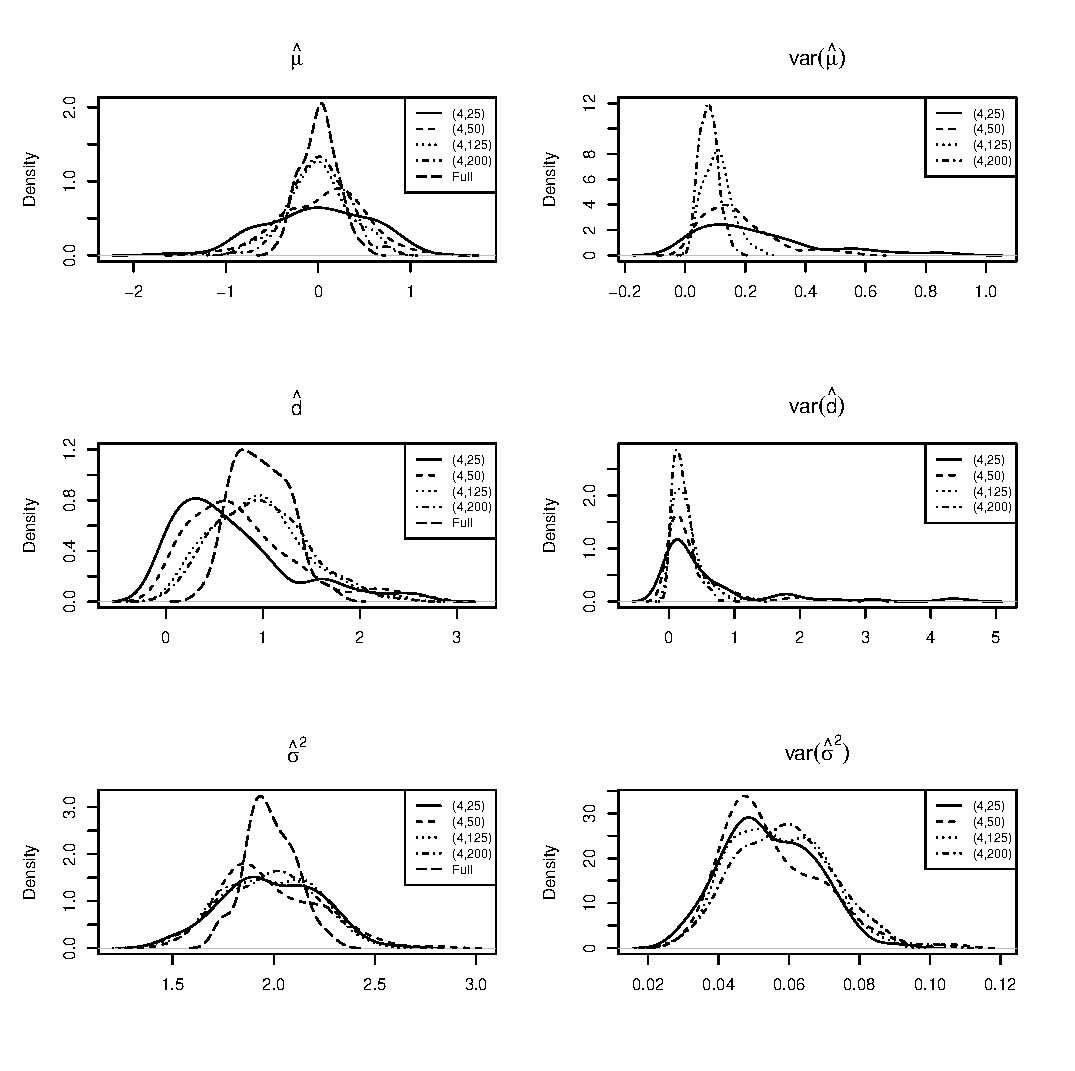
\includegraphics[width=\textwidth]{aCS150.eps}
\caption{\small \linespread{1.1} First simulation study. Setting 1. Split-specific results.} \label{CS150}
\end{figure}
\begin{figure}[!t]
\centering
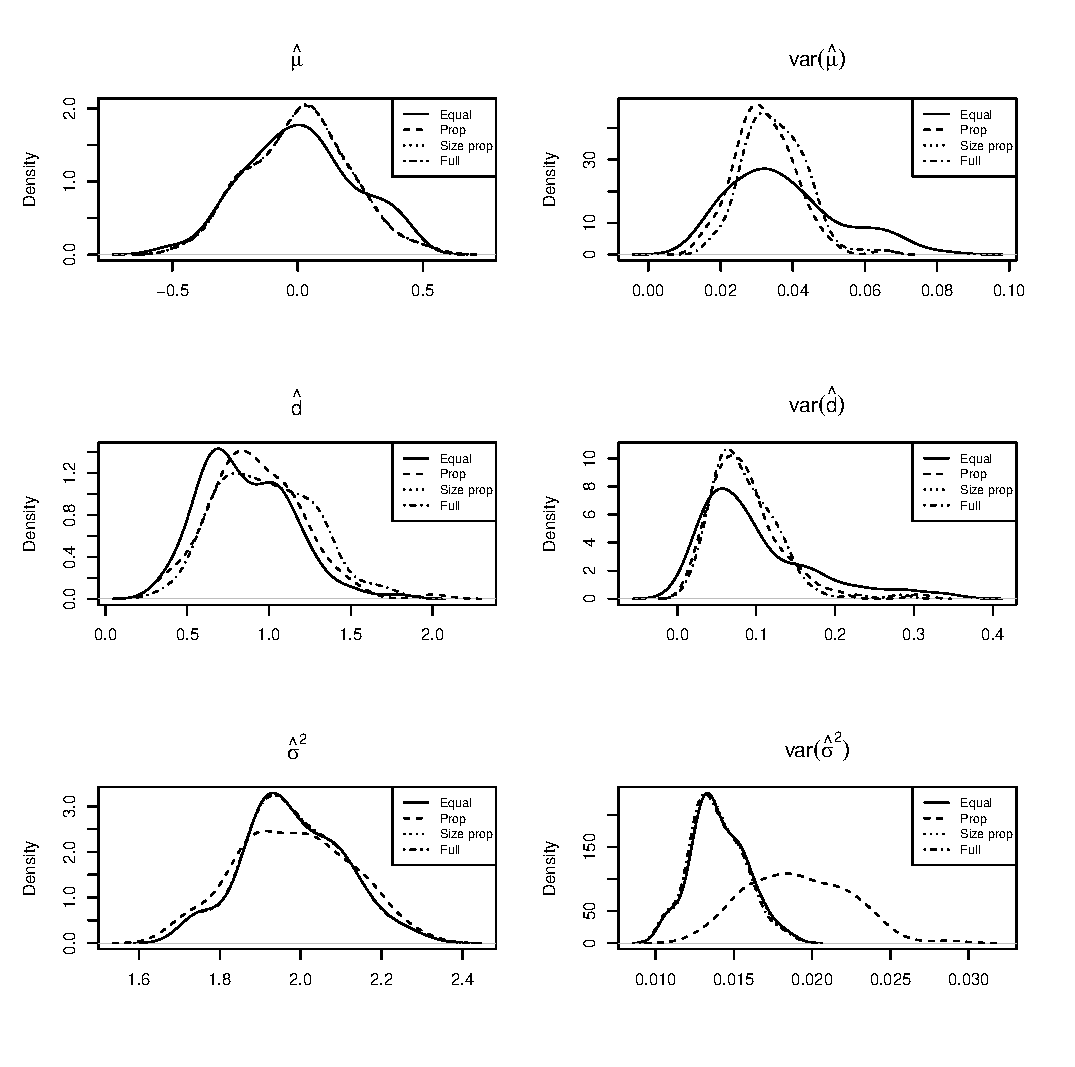
\includegraphics[width=\textwidth]{aCS150COMB.eps}
\caption{\small \linespread{1.1} First simulation study. Setting 1. Combining the results from the four splits, using equal, proportional, and size proportional weights. This is compared with full maximum likelihood.} \label{CS150COMB}
\end{figure}



\subsection[Setting 2]{Setting 2: different $c_k\cdot n_k$, equal $c_k$, different $n_k$}

To see the effect of split size, the following choices are made:
$(c_1,n_1)=(4,25)$,  $(c_2,n_2)=(4,50)$,  $(c_3,n_3)=(4,125)$, and $(c_4,n_4)=(4,250)$.
As a consequence, the size of the splits will be $100$, $200$, $500$, and $1000$, respectively. Table~\ref{tab_diff1} summarized the results, with graphical displays presented in Figures~\ref{CS_diff1} and \ref{CS_diff_comb}.
\begin{table}[t]
\centering
\caption{\small \linespread{1.1} First simulation study. Setting 2. Average of split-specific and combined (weighted) parameters and their precision estimates.}
\label{tab_diff1}

\vspace*{2mm}

\def\arraystretch{1} \begin{tabular}{rrrrrrr}
\hline  \hline
  & \multicolumn{1}{c}{$\mu$} & \multicolumn{1}{c}{\mbox{var}($\mu$)} & \multicolumn{1}{c}{$d$} & \multicolumn{1}{c}{\mbox{var}($d$)} & \multicolumn{1}{c}{$\sigma^2$} & \multicolumn{1}{c}{\mbox{var}($\sigma^2$)} \\
\hline
split1 & -0.02515 & 0.05227 & 0.83440 & 0.52423 & 2.00347 & 0.00730 \\
  split2 & 0.01287 & 0.05157 & 0.86891 & 0.57904 & 1.97285 & 0.00160 \\
  split3 & 0.06812 & 0.03586 & 0.74147 & 0.23681 & 2.00165 & 0.00026 \\
  split4 & -0.03676 & 0.02979 & 0.68241 & 0.14117 & 1.99216 & 0.00006 \\
  \hline
 Equal & 0.00477 & 0.05111 & 0.78180 & 0.14770 & 1.99253 & 0.00935 \\
  Prop & 0.00477 & 0.05111 & 0.78180 & 0.14770 & 1.99253 & 0.00935 \\
  Size prop & -0.00147 & 0.07139 & 0.72798 & 0.16585 & 1.99328 & 0.00447 \\
  Full & 0.00530 & 0.06339 & 0.89599 & 0.14604 & 1.99333 & 0.00446 \\
 \hline
\hline
\end{tabular}
\end{table}

\begin{figure}[!t]
\centering
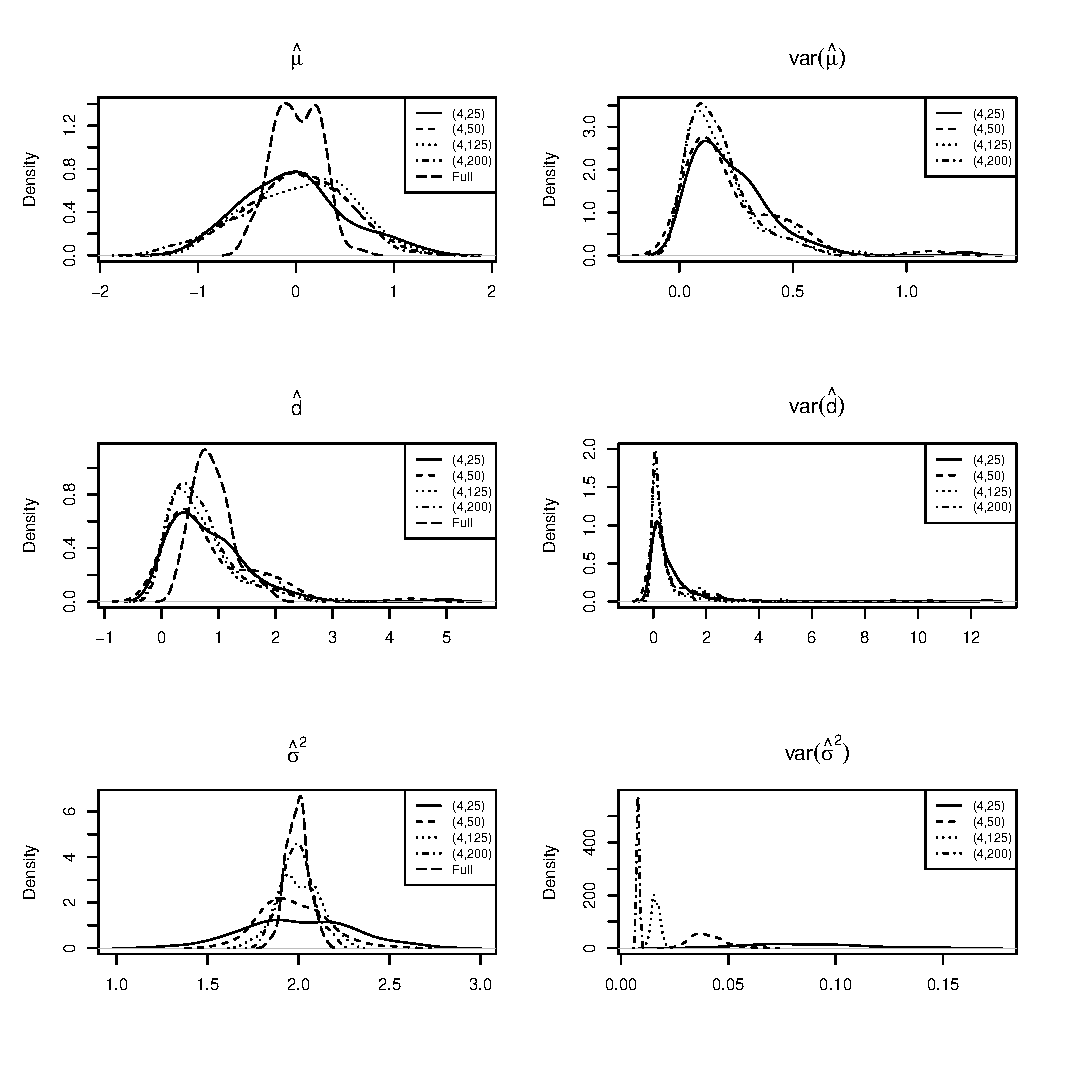
\includegraphics[width=\textwidth]{aCS_diff1.eps}
\caption{\small \linespread{1.1} First simulation study. Setting 2. Split-specific results.} \label{CS_diff1}
\end{figure}
\begin{figure}[!t]
\centering
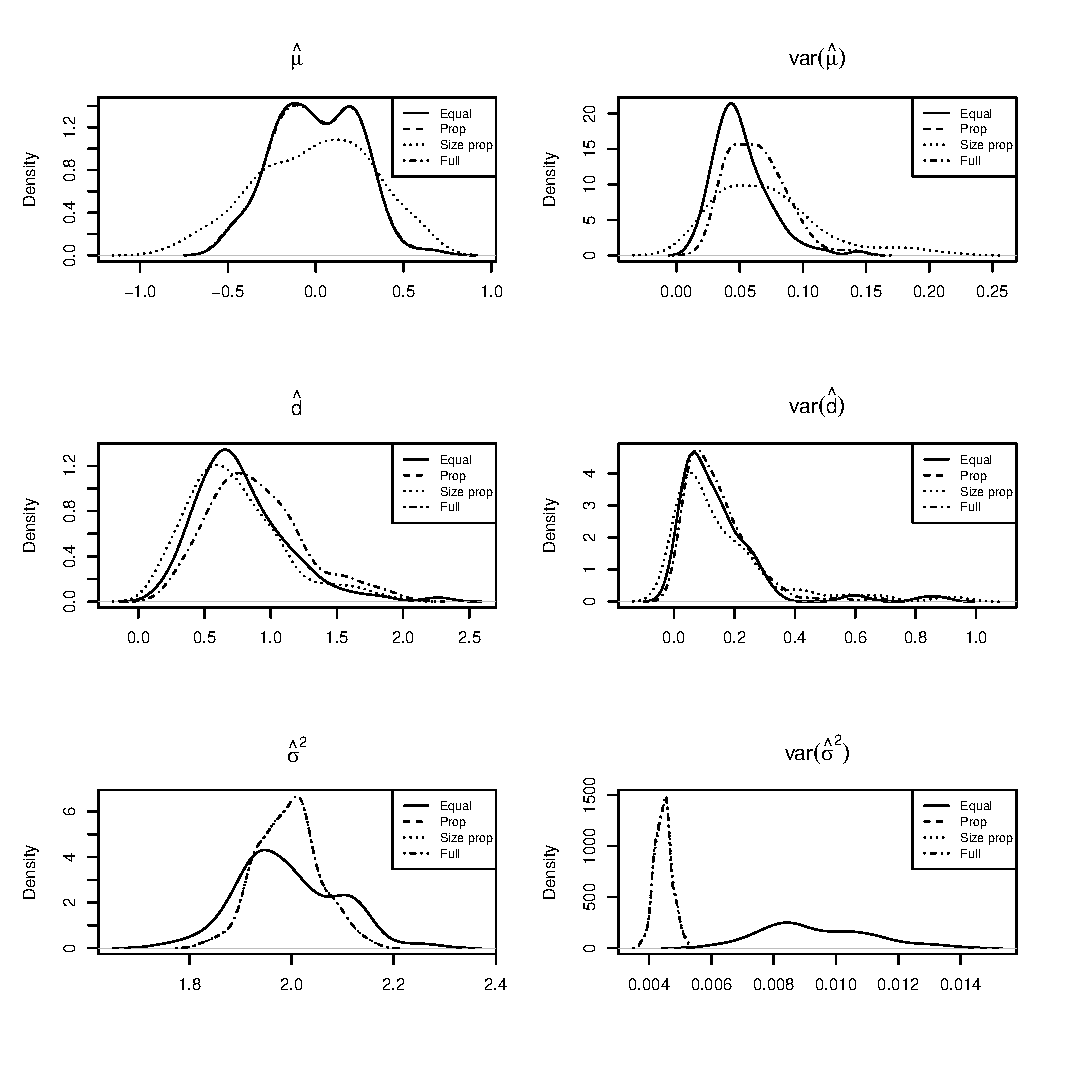
\includegraphics[width=\textwidth]{aCS_diff_comb.eps}
\caption{\small \linespread{1.1} First simulation study. Setting 2. Combining the results from the four splits, using equal, proportional, and size proportional weights. This is compared with full maximum likelihood.} \label{CS_diff_comb}
\end{figure}


\subsection[Setting 3]{Setting 3: different $c_k\cdot n_k$, different $c_k$, equal $n_k$}
We now choose: $(c_1,n_1)=(10,20)$,  $(c_2,n_2)=(20,20)$, $(c_3,n_3)=(50,20)$, and
$(c_4,n_4)=(100,20)$. Table~\ref{tab_diff2} summarizes the results. Graphs can be found in Figures~\ref{CS_diff2} and \ref{CS_diff_comb2}.
\begin{table}[h]
\centering
\caption{\small \linespread{1.1} First simulation study. Setting 3. Average of split-specific and combined (weighted) parameters and their precision estimates.}
\label{tab_diff2}

\vspace*{2mm}

\def\arraystretch{1} \begin{tabular}{rrrrrrr}
  \hline\hline
  & \multicolumn{1}{c}{$\mu$} & \multicolumn{1}{c}{\mbox{var}($\mu$)} & \multicolumn{1}{c}{$d$} & \multicolumn{1}{c}{\mbox{var}($d$)} & \multicolumn{1}{c}{$\sigma^2$} & \multicolumn{1}{c}{\mbox{var}($\sigma^2$)} \\
  \hline
split1 & 0.00343 & 0.00900 & 0.84739 & 0.05169 & 2.02445 & 0.00190 \\
  split2 & 0.02553 & 0.00304 & 1.00224 & 0.01754 & 2.01962 & 0.00047 \\
  split3 & -0.00010 & 0.00045 & 0.95794 & 0.00212 & 1.99765 & 0.00007 \\
  split4 & 0.01151 & 0.00012 & 1.01226 & 0.00064 & 1.98944 & 0.00002 \\
   \hline
 \hline
Equal & 0.01009 & 0.01139 & 0.95496 & 0.02694 & 2.00779 & 0.00486 \\
  Prop & 0.00939 & 0.00604 & 0.98690 & 0.01369 & 1.99702 & 0.00234 \\
  Size prop & 0.00939 & 0.00604 & 0.98690 & 0.01369 & 1.99702 & 0.00234 \\
  Full & 0.00939 & 0.00614 & 1.00487 & 0.01372 & 1.99702 & 0.00233 \\
 \hline\hline
\end{tabular}
\end{table}


\begin{figure}[!t]
\centering
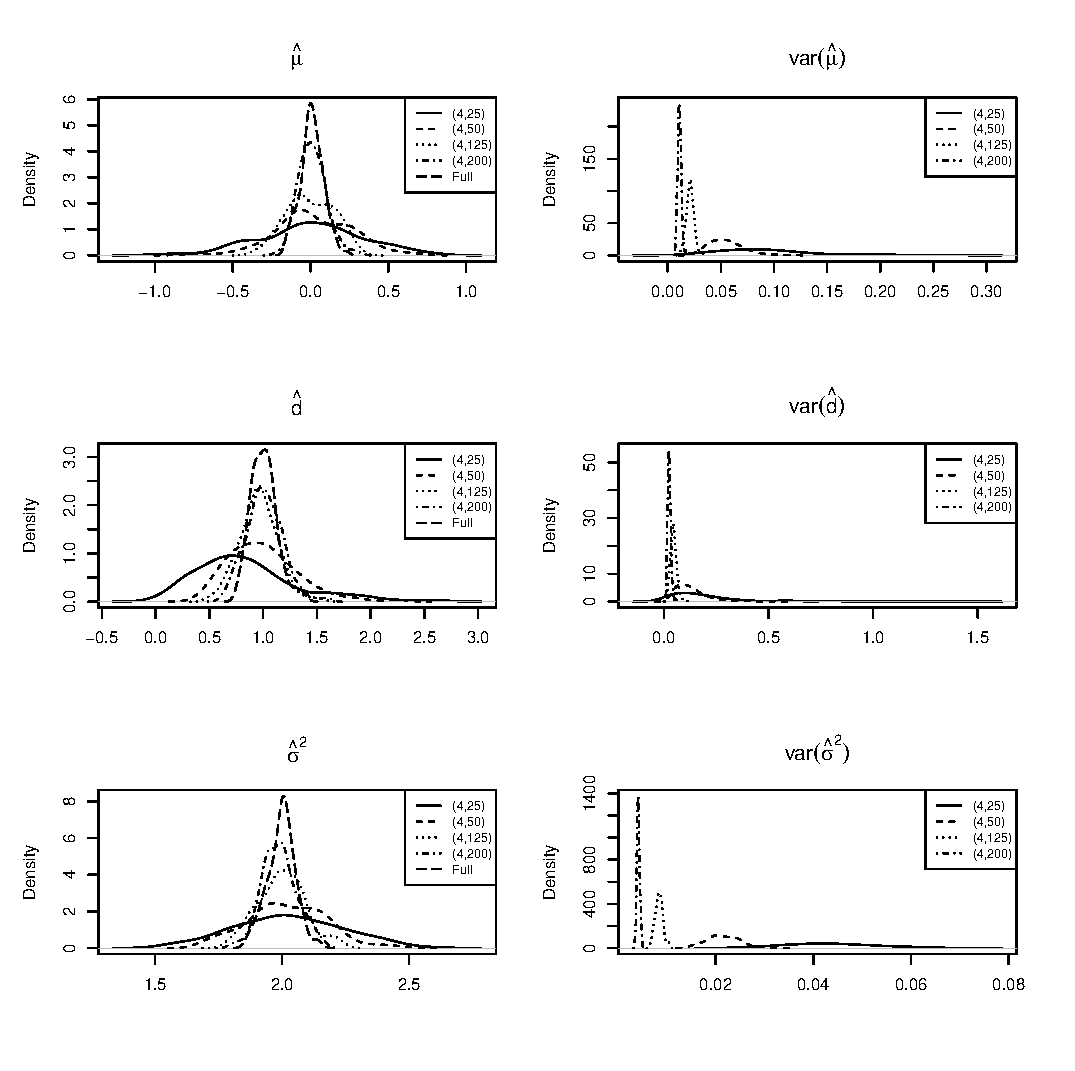
\includegraphics[width=\textwidth]{aCS_diff2.eps}
\caption{\small \linespread{1.1} First simulation study. Setting 3. Split-specific results. \label{CS_diff2}}
\end{figure}
\begin{figure}[!t]
\centering
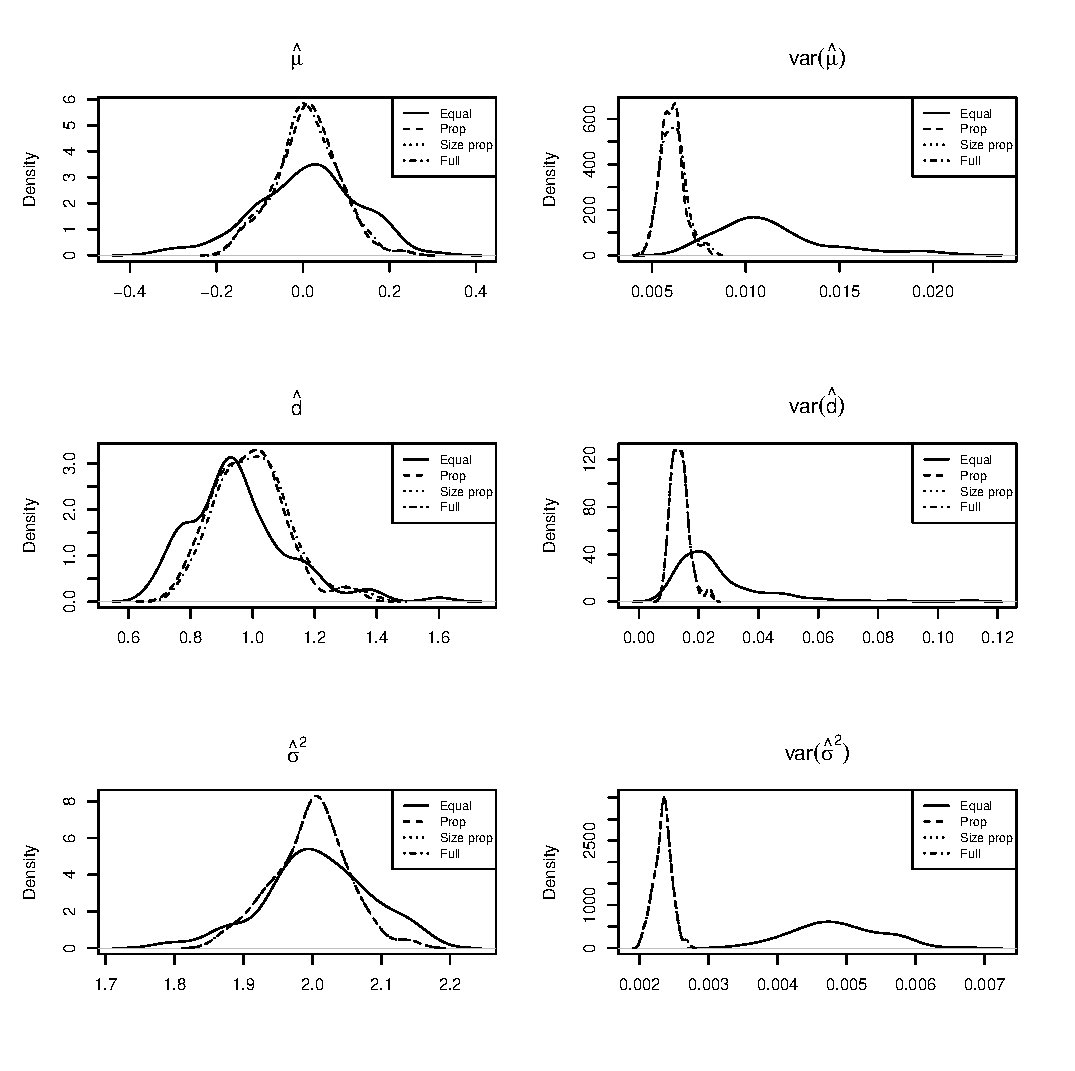
\includegraphics[width=\textwidth]{aCS_diff_comb2.eps}
\caption{\small \linespread{1.1} First simulation study. Setting 3. Combining the results from the four splits, using equal, proportional, and size proportional weights. This is compared with full maximum likelihood.} \label{CS_diff_comb2}
\end{figure}


\subsection{Optimal, approximate optimal, and iterated optimal weights}

Optimal weights were discussed in Section~6.1.1.
%\ref{owcs}. 
When we plug the MLE's into the optimal weights, the result of using these weights is the MLE's itself. Of course, this is a circular reasoning, which is why one needs to resort to, for example, the approximate or iterated optimal weights derived in Section~6.1.2.
%\ref{iaow}. 
For both of these, using Settings~1--3, we conducted simulations. They are reported in Figures~\ref{Setting1_opt}--\ref{Setting3_opt}.
\begin{figure}[!t]
\centering
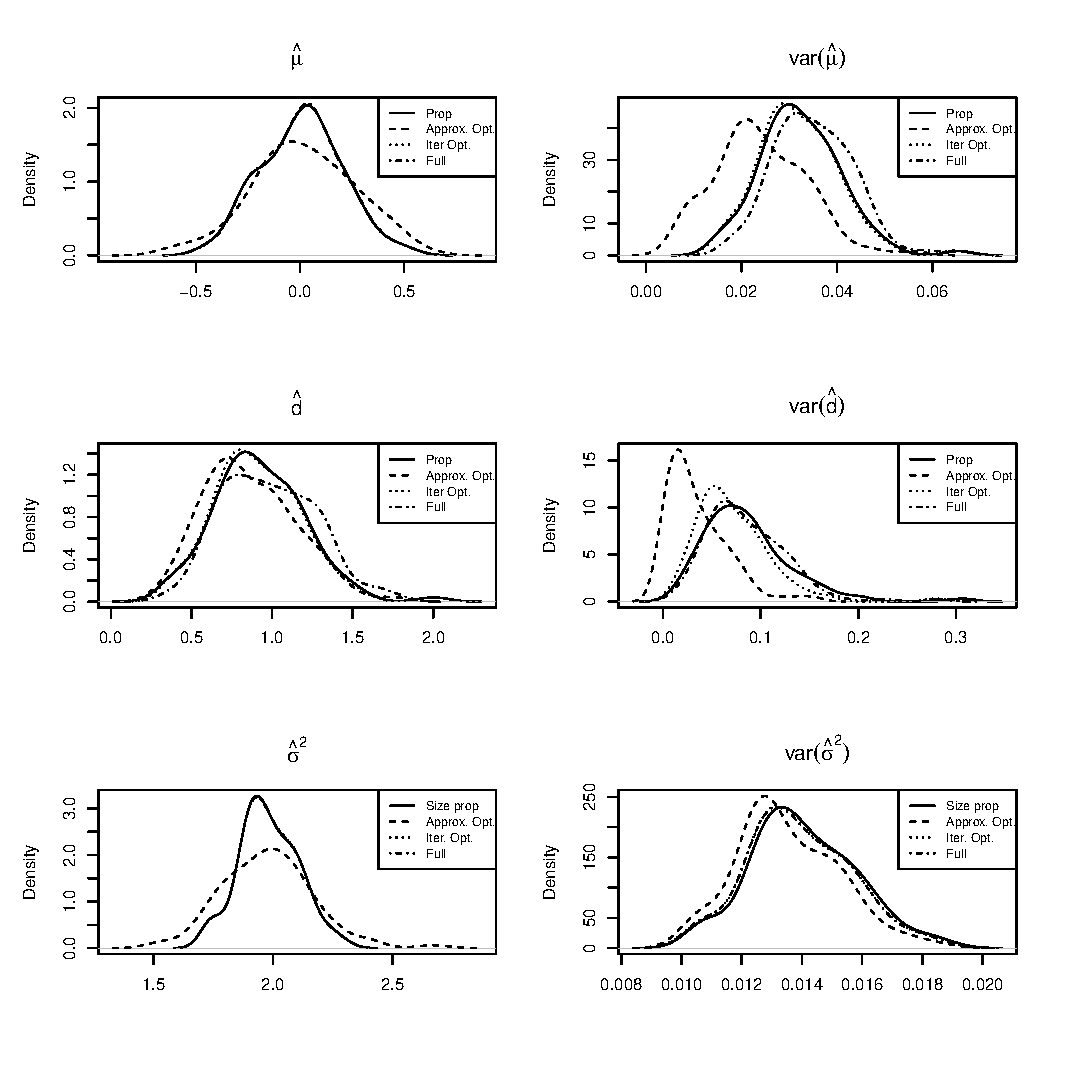
\includegraphics[width=\textwidth]{aSetting1_opt.eps}
\caption{\small \linespread{1.1} First simulation study. Setting 1. (Size) proportional, approximate, and iterated optimal weights, as well as full maximum likelihood.} \label{Setting1_opt}
\end{figure}
\begin{figure}[!t]
\centering
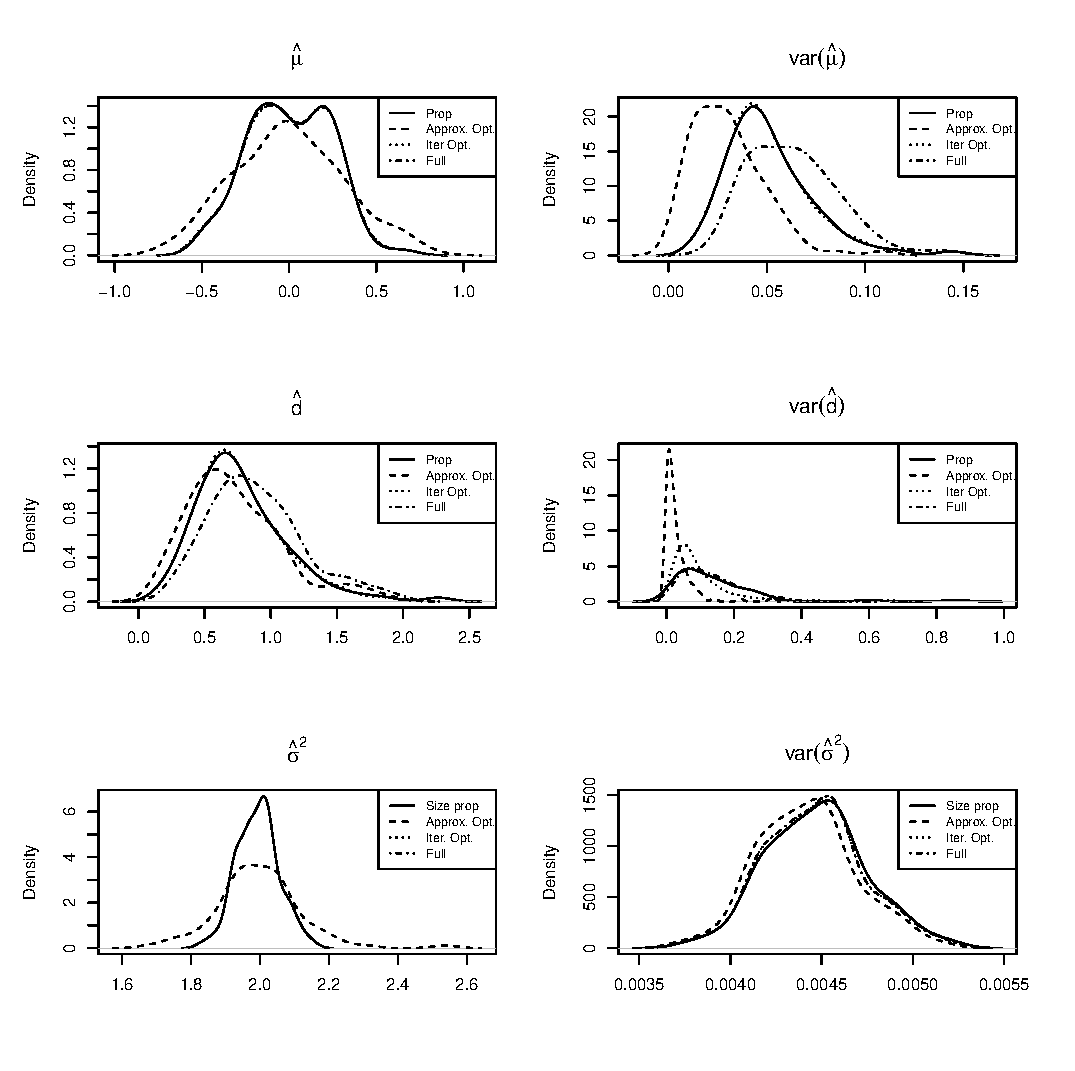
\includegraphics[width=\textwidth]{aSetting2_opt.eps}
\caption{\small \linespread{1.1} First simulation study. Setting 2. (Size) proportional, approximate, and iterated optimal weights, as well as full maximum likelihood.} \label{Setting2_opt}
\end{figure}
\begin{figure}[!t]
\centering
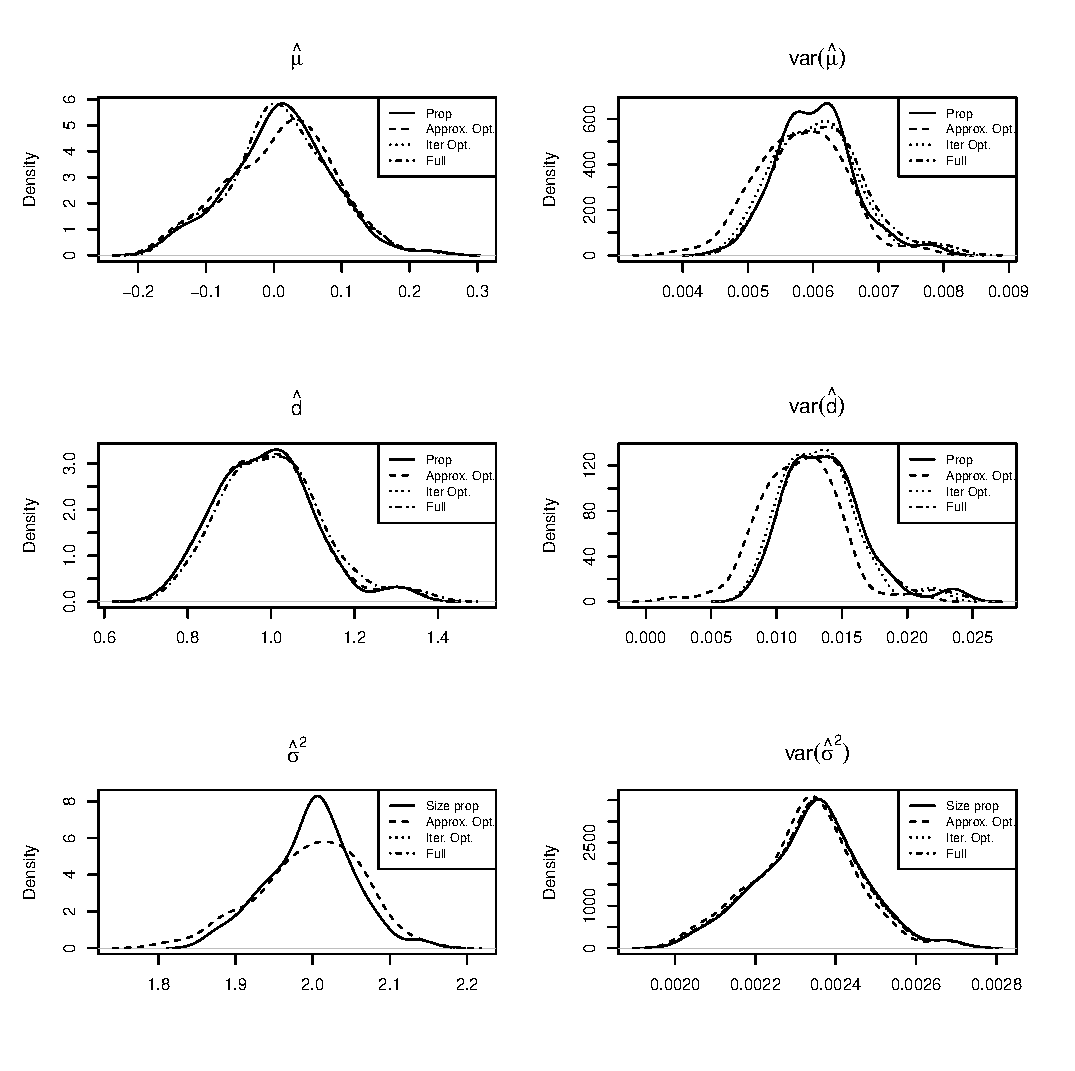
\includegraphics[width=\textwidth]{aSetting3_opt.eps}
\caption{\small \linespread{1.1} First simulation study. Setting 3. (Size) proportional, approximate, and iterated optimal weights, as well as full maximum likelihood.} \label{Setting3_opt}
\end{figure}

It is noteworthy that the behavior of the iterated optimal weights depends on $c_k$ and $n_k$. First, they often but not always converge in a single iteration; the maximum number of iterations observed in our simulations being~6. Second, the iterated optimal weights  converge to size optimal weights for $\sigma^2$ and to proportional weights for $d$.

Taken together, it follows that both approximately optimal and iterated optimal weights provide excellent results. The specific attraction of the approximate optimal weights is that they obviate the need for iteration, which is a factor of stability and speed.

\setcounter{equation}{0}
\section{Details about the second simulation study}
\label{simapptwee}

The aim of this study is to compare the proposed method to two alternatives: 
\begin{enumerate}
\item full maximum likelihood;
\item the proposed  sample-splitting method, allowing for closed forms;
\item using multiple imputation (MI) first, to render the clusters of equal sizes, and then apply closed-form solutions to the augmented balanced data, together with the combination rules.
\end{enumerate}

\subsection{Simulation plan}

In order to study the effect of cluster sizes ($n_k$) and number of clusters of each size ($c_k$), 5 different configurations are considered:
\begin{description}
\item[Config.~1.] $c_k=(15,25,30,20,10)$, $n_k=(8,5,3,9,15)$;
\item[Config.~2.] $c_k=(150,250,300,200,100)$, $n_k=(8,5,3,9,15)$;
\item[Config.~3.] $c_k=(1500,2500,3000,2000,1000)$, $n_k=(8,5,3,9,15)$;
\item[Config.~4.] $c_k=(15,25,30,20,10)$, $n_k=(80,50,30,90,150)$;
\item[Config.~5.] $c_k=(15,25,30,20,10)$, $n_k=(800,500,300,900,1500)$.
\end{description}
 Each configuration is repeated $100$ times.

Each cluster is generated from a CS model with $\mu_0=0$, $d_0=1$, and $\sigma^2_0=4$. 

For estimating the parameters using the full unbalanced data, PROC MIXED in SAS (Version 9.4) is used with the covariance structure in the REPEATED statement set to {\tt{type=cs}}.


The closed form solutions and their variances are implemented in {\tt R} in three different ways. First, the formulas  are implemented directly using `for' loops. Following the ideas in \cite{sikorska2013_2}, it might be faster to replace `for' loops with vectorized computation. For $\widehat{\mu}_k$ it is straightforward, since one just needs to compute an arithmetic average. If $Z$ is a $n_k$ times $c_k$ matrix with its $i$th column defined as $Z_i^{(k)}=\left(Y_i^{(k)} - \mu_k \mathbf{1}_{n_k} \right)$, then computing $\sum_{i=1}^ {c_k}  Z_i^{(k)'} Z_i^{(k)}$  is equivalent to replacing each element in matrix $Z$ by its square, and then sum over the sum of its columns. Furthermore, $J_{n_k} Z_i^{(k)}$ would simply compute the sum of columns in matrix $Z$. Therefore, $\sum_{i=1}^{c_k} Z_i^{(k)'} J_{n_k} Z_I^{(k)}$ is equivalent to post-multiplying $Z$ by the sum of its columns and then sum over this vector. In this way, within each split, the parameters can be estimated avoiding `for' loops. 

Second, it is also possible to find the estimates for all of the splits at once instead of computing them separately. 

A third way consists of calculating all the estimates together and not split by split in a `for' loop. This approach is possible via imposing balance through adding missing values in the matrix but, when multiplying and summing, ignoring the missing values. This is very easy in {\tt R}. 

We will compare computation time between these three approaches, for the five configurations.

Additionally, to combine the results from sample splitting, the same
weights as used in the case study are considered here as well: equal, proportional, approximate scalar, scalar, and approximate optimal. In the case of the approximate optimal weights both simple and proper variances are calculated. 

For the multiple imputation based approach, $M=20$ imputations are considered and the conventional combination rules applied.

 Note that the MI approach cannot be used with configurations 1, 4, and 5, because the number of available subjects in the observed dataset is less than the number of repeated measurements, leading to a singular covariance matrix. From the remaining configurations 2 and 3, we have chosen \#2, which implies smaller numbers and hence is more challenging.

For each configuration we report three results: the estimated parameters, their standard errors, and the mean square error (MSE). Furthermore, we report computation time. 

\subsection{Simulation results}

\begin{table}[ht]
\centering
\caption{\small \linespread{1.1} Second simulation study. Mean, standard deviation (S.D.) and MSE for $\mu$ among 100 replications for each configuration using different combination weights comparing with full sample MLE.}
\label{tab_mu_est}

\vspace*{2mm}


\resizebox{\textwidth}{!}{%
\def\arraystretch{1} \begin{tabular}{cccccccc}
  \hline\hline
Config.& & Equal & Prop & Approx.~sc. & Scalar & Approx.~opt. & ML \\ 
  \hline
 & Mean & -1.72277E-02 & -1.51605E-02 & -1.51605E-02 & -1.21296E-02 & -1.21296E-02 & -1.56028E-02 \\ 
1 & S.D. & (1.32751E-01) & (1.28989E-01) & (1.28989E-01) & (1.32435E-01) & (1.32435E-01) & (1.29150E-01) \\ 
 & MSE & 1.77434E-02 & 1.67015E-02 & 1.67015E-02 & 1.75108E-02 & 1.75108E-02 & 1.67564E-02 \\ 
 & Mean & -9.39926E-04 & 6.93419E-04 & 6.93419E-04 & 1.27613E-03 & 1.27613E-03 & 7.59533E-04 \\ 
2 & S.D. & (3.93526E-02) & (3.95534E-02) & (3.95534E-02) & (3.84321E-02) & (3.84321E-02) & (3.83996E-02) \\ 
 & MSE & 1.53403E-03 & 1.54930E-03 & 1.54930E-03 & 1.46389E-03 & 1.46389E-03 & 1.46036E-03 \\ 
 & Mean & -8.30934E-04 & -1.25609E-03 & -1.25609E-03 & -1.26810E-03 & -1.26810E-03 & -1.31356E-03 \\ 
3 & S.D.& (1.44839E-02) & (1.47545E-02) & (1.47545E-02) & (1.41310E-02) & (1.41310E-02) & (1.41704E-02) \\ 
 & MSE & 2.08376E-04 & 2.17095E-04 & 2.17095E-04 & 1.99298E-04 & 1.99298E-04 & 2.00517E-04 \\ 
 & Mean & 9.30928E-03 & 2.53713E-03 & 2.53713E-03 & 8.29367E-03 & 8.29367E-03 & 2.82086E-03 \\ 
4 & S.D. & (9.26881E-02) & (8.32009E-02) & (8.32009E-02) & (9.76672E-02) & (9.76672E-02) & (8.28999E-02) \\ 
 & MSE & 8.59183E-03 & 6.85960E-03 & 6.85960E-03 & 9.51227E-03 & 9.51227E-03 & 6.81163E-03 \\ 
 & Mean & 9.77532E-03 & 1.02173E-02 & 1.02173E-02 & 8.72381E-03 & 8.72381E-03 & 1.02422E-02 \\ 
5 & S.D. & (1.09769E-01) & (1.04876E-01) & (1.04876E-01) & (1.04982E-01) & (1.04982E-01) & (1.04847E-01) \\ 
 & MSE & 1.20243E-02 & 1.09934E-02 & 1.09934E-02 & 1.09872E-02 & 1.09872E-02 & 1.09880E-02 \\ 
   \hline\hline
\end{tabular}}
\end{table}



\begin{table}[ht]
\centering
\caption{\small \linespread{1.1} Second simulation study. Mean and standard deviation (S.D.) for standard errors of $\mu$ estimates in 100 replications for each configuration using different combination weights comparing with full sample MLE.}
\label{tab_mu_std}

\vspace*{2mm}

\resizebox{\textwidth}{!}{%
\def\arraystretch{1} \begin{tabular}{ccccccccc}
  \hline\hline
Config.& & Equal & Prop & Approx.~sc. & Scalar & Simple opt. & Proper opt. & ML \\ 
  \hline
1  &Mean & 1.29844E-01 & 1.29733E-01 & 1.29733E-01 & 1.20593E-01 & 1.20593E-01 & 1.41085E-01 & 1.29648E-01 \\ 
  &S.D.& (1.18175E-02) & (1.07496E-02) & (1.07496E-02) & (1.09122E-02) & (1.09122E-02) & (2.25155E-02) & (9.95614E-03) \\ 
2  &Mean & 4.23655E-02 & 4.23056E-02 & 4.23056E-02 & 4.11657E-02 & 4.11657E-02 & 4.12635E-02 & 4.14298E-02 \\ 
  &S.D.& (1.08386E-03) & (8.88747E-04) & (8.88747E-04) & (8.71465E-04) & (8.71465E-04) & (8.90259E-04) & (8.66432E-04) \\ 
3  &Mean & 1.34008E-02 & 1.33822E-02 & 1.33822E-02 & 1.30725E-02 & 1.30725E-02 & 1.30728E-02 & 1.30799E-02 \\ 
  &S.D.& (1.21880E-04) & (9.92324E-05) & (9.92324E-05) & (9.68871E-05) & (9.68871E-05) & (9.68974E-05) & (9.62652E-05) \\ 
4  &Mean & 1.06373E-01 & 1.01232E-01 & 1.01232E-01 & 9.60807E-02 & 9.60807E-02 & 3.30358E-01 & 1.03382E-01 \\ 
  &S.D.& (9.80278E-03) & (7.26031E-03) & (7.26031E-03) & (8.36242E-03) & (8.36242E-03) & (1.39042E-01) & (7.17708E-03) \\ 
4  &Mean & 1.05176E-01 & 9.84615E-02 & 9.84615E-02 & 9.45066E-02 & 9.45066E-02 & 2.81427E+00 & 1.00533E-01 \\ 
  &S.D.& (1.10711E-02) & (8.18259E-03) & (8.18259E-03) & (8.14229E-03) & (8.14229E-03) & (1.41211E+00) & (8.28537E-03) \\ 
\hline\hline  
\end{tabular}}
\end{table}




















\begin{figure}
\centering
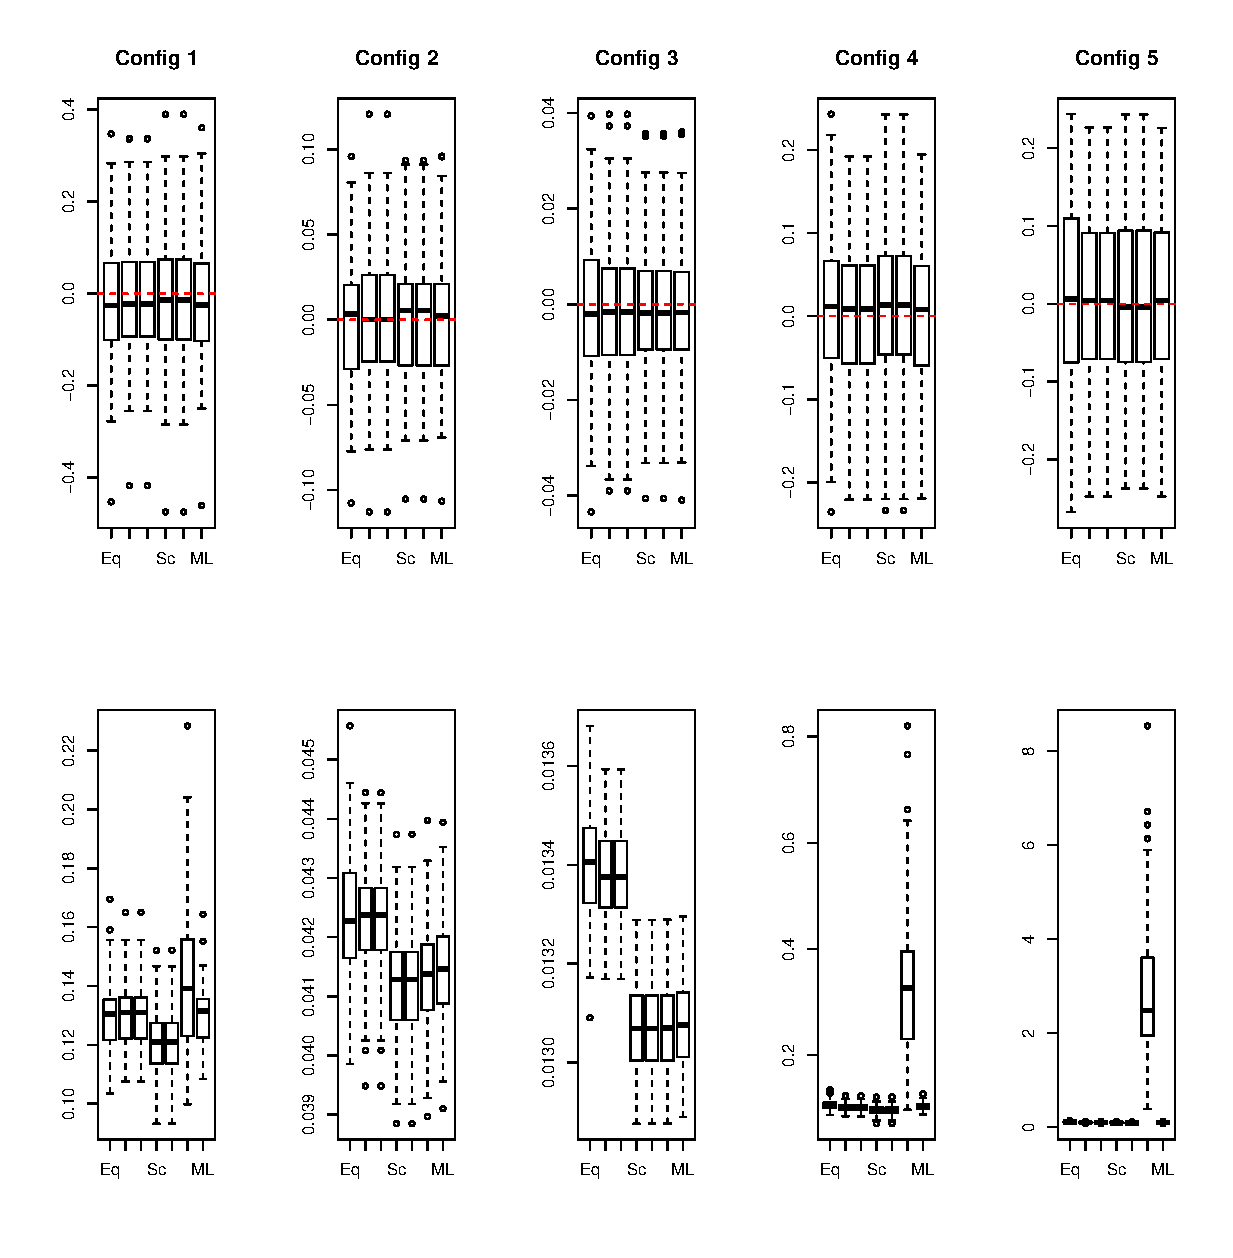
\includegraphics[width=\textwidth]{fig_mu.eps}
\caption{\small \linespread{1.1}  Second simulation study. Estimates for $\mu$ (first row) and its standard error (second row).} \label{fig_mu}
\end{figure}




\begin{table}[ht]
\centering
\caption{\small \linespread{1.1} Second simulation study. Mean, standard deviation (S.D.) and MSE for $d$ estimates in 100 replications for each configuration using different combination weights comparing with full sample MLE.}
\label{tab_d_est}

\vspace*{2mm}

\resizebox{\textwidth}{!}{%
\def\arraystretch{1} \begin{tabular}{cccccccc}
  \hline\hline
Config.& & Equal & Prop & Approx.~sc. & Scalar & Approx.~opt & ML \\ 
  \hline
 & Mean & 9.09580E-01 & 9.00788E-01 & 9.00788E-01 & 6.63293E-01 & 6.71111E-01 & 9.86549E-01 \\ 
1 & S.D. & (2.66885E-01) & (2.99736E-01) & (2.99736E-01) & (2.70556E-01) & (2.79060E-01) & (2.55874E-01) \\ 
 & MSE & 7.86910E-02 & 9.87862E-02 & 9.87862E-02 & 1.85840E-01 & 1.85264E-01 & 6.49975E-02 \\ 
 & Mean & 9.98984E-01 & 9.97534E-01 & 9.97534E-01 & 9.72269E-01 & 9.73771E-01 & 1.00712E+00 \\ 
2 & S.D. & (7.44958E-02) & (8.28143E-02) & (8.28143E-02) & (7.28186E-02) & (7.22762E-02) & (7.08463E-02) \\ 
 & MSE & 5.49515E-03 & 6.79570E-03 & 6.79570E-03 & 6.01854E-03 & 5.85958E-03 & 5.01969E-03 \\ 
 & Mean & 1.00004E+00 & 9.99697E-01 & 9.99697E-01 & 9.97218E-01 & 9.97153E-01 & 1.00019E+00 \\ 
3 & S.D. & (2.61046E-02) & (2.82480E-02) & (2.82480E-02) & (2.48989E-02) & (2.48068E-02) & (2.44715E-02) \\ 
 & MSE & 6.74637E-04 & 7.90063E-04 & 7.90063E-04 & 6.21496E-04 & 6.17332E-04 & 5.92900E-04 \\ 
 & Mean & 9.40257E-01 & 9.50756E-01 & 9.50756E-01 & 7.65219E-01 & 7.65362E-01 & 9.96005E-01 \\ 
4 & S.D. & (1.53414E-01) & (1.48216E-01) & (1.48216E-01) & (1.91865E-01) & (1.91614E-01) & (1.49451E-01) \\ 
 & MSE & 2.68697E-02 & 2.41734E-02 & 2.41734E-02 & 9.15661E-02 & 9.14038E-02 & 2.21282E-02 \\ 
 & Mean & 9.63459E-01 & 9.68182E-01 & 9.68182E-01 & 8.21266E-01 & 8.21270E-01 & 1.00958E+00 \\ 
5 & S.D. & (1.73767E-01) & (1.63471E-01) & (1.63471E-01) & (1.72162E-01) & (1.72163E-01) & (1.69235E-01) \\ 
 & MSE & 3.12283E-02 & 2.74677E-02 & 2.74677E-02 & 6.12894E-02 & 6.12881E-02 & 2.84459E-02 \\ 
\hline
   \hline
\end{tabular}}
\end{table}



\begin{table}[ht]
\centering
\caption{\small \linespread{1.1}Second simulation study. Mean and standard deviation (S.D.) for standard errors of $d$ estimates in 100 replications for each configuration using different combination weights comparing with full sample MLE.}
\label{tab_d_std}

\vspace*{2mm}

\resizebox{\textwidth}{!}{%
\def\arraystretch{1} \begin{tabular}{ccccccccc}
  \hline\hline
Config.& & Equal & Prop. & Approx.~sc. & Scalar & Simple opt. & Proper opt. & ML \\ 
  \hline
1 & Mean & 5.30888E-01 & 6.76159E-01 & 6.76159E-01 & 4.83519E-01 & 1.95328E-01 & 4.66561E+00 & 2.36408E-01 \\ 
 & S.D. & (1.00495E-01) & (1.66365E-01) & (1.66365E-01) & (1.10589E-01) & (4.01066E-02) & (1.40173E+00) & (3.91752E-02) \\ 
2 & Mean & 1.60365E-01 & 2.03126E-01 & 2.03126E-01 & 1.45284E-01 & 7.48056E-02 & 1.47955E+00 & 7.60798E-02 \\ 
 & S.D. & (8.29444E-03) & (1.42616E-02) & (1.42616E-02) & (8.70034E-03) & (3.35411E-03) & (1.31587E-01) & (3.26483E-03) \\ 
3 & Mean & 5.02596E-02 & 6.34861E-02 & 6.34861E-02 & 4.56061E-02 & 2.39463E-02 & 4.67989E-01 & 2.39748E-02 \\ 
 & S.D. & (8.43976E-04) & (1.44201E-03) & (1.44201E-03) & (8.34510E-04) & (3.68251E-04) & (1.24414E-02) & (3.66865E-04) \\ 
4 & Mean & 1.62410E-01 & 1.59656E-01 & 1.59656E-01 & 1.34256E-01 & 1.24552E-01 & 2.35351E-01 & 1.51740E-01 \\ 
 & S.D. & (2.83009E-02) & (2.05482E-02) & (2.05482E-02) & (2.31559E-02) &(2.51091E-02) & (3.00109E-02) & (2.11541E-02) \\ 
5 & Mean & 1.54122E-01 & 1.43313E-01 & 1.43313E-01 & 1.22117E-01 & 1.22024E-01 & 1.70868E-01 & 1.43764E-01 \\ 
 & S.D. & (3.48725E-02) & (2.50371E-02) & (2.50371E-02) & (2.30972E-02)& (2.31064E-02) & (3.70951E-02) & (2.38992E-02) \\ 
   \hline\hline
\end{tabular}}
\end{table}


\begin{figure}
\centering
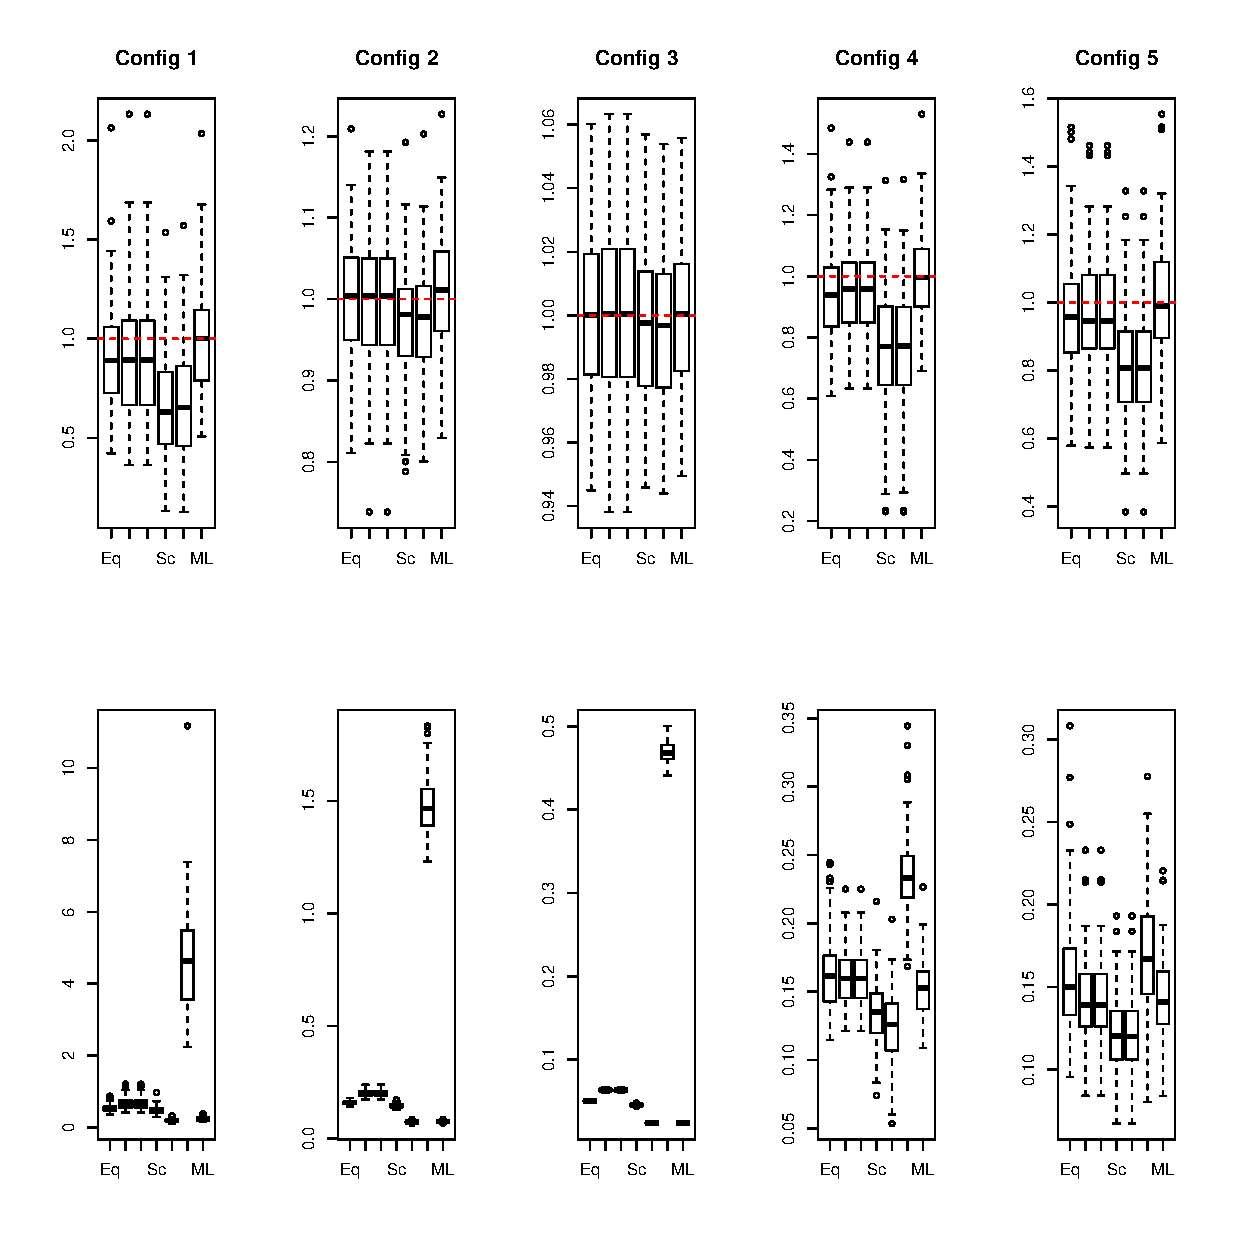
\includegraphics[width=\textwidth]{fig_d.eps}
\caption{\small \linespread{1.1} Second simulation study. Estimates for $d$ (first row) and standard errors ( second row).} \label{fig_d}
\end{figure}






\begin{table}[ht]
\centering
\caption{\small \linespread{1.1}Second simulation study. Mean, standard deviation (S.D.) and MSE for $\sigma^2$ estimates in 100 replications for each configuration using different combination weights comparing with full sample MLE.}
\label{tab_sigma2_est}

\vspace*{2mm}

\resizebox{\textwidth}{!}{%
\def\arraystretch{1} \begin{tabular}{cccccccc}
  \hline\hline
Config.& & Equal & Prop. & Approx.~sc. & Scalar & Approx.~opt. & ML \\ 
  \hline
 & Mean & 3.98608E+00 & 3.99739E+00 & 3.98571E+00 & 3.98364E+00 & 3.87487E+00 & 3.98075E+00 \\ 
1 & S.D. & (2.50882E-01) & (2.95821E-01) & (2.35138E-01) & (2.33650E-01) & (2.38167E-01) & (2.30477E-01) \\ 
 & MSE & 6.25062E-02 & 8.66420E-02 & 5.49414E-02 & 5.43140E-02 & 7.18141E-02 & 5.29588E-02 \\ 
 & Mean & 4.00184E+00 & 4.00681E+00 & 4.00177E+00 & 4.00087E+00 & 3.99027E+00 & 4.00064E+00 \\ 
2 & S.D. & (7.85190E-02) & (9.05849E-02) & (7.57443E-02) & (7.56486E-02) & (7.50477E-02) & (7.51739E-02) \\ 
 & MSE & 6.10698E-03 & 8.16998E-03 & 5.68296E-03 & 5.66624E-03 & 5.67055E-03 & 5.59502E-03 \\ 
 & Mean & 4.00509E+00 & 4.00491E+00 & 4.00575E+00 & 4.00590E+00 & 4.00472E+00 & 4.00587E+00 \\ 
3 & S.D. & (2.45760E-02) & (2.82395E-02) & (2.36027E-02) & (2.36983E-02) & (2.37694E-02) & (2.36697E-02) \\ 
 & MSE & 6.23828E-04 & 8.13646E-04 & 5.84605E-04 & 5.90806E-04 & 5.81652E-04 & 5.89081E-04 \\ 
 & Mean & 4.01402E+00 & 4.01190E+00 & 4.01302E+00 & 4.01304E+00 & 4.00363E+00 & 4.01306E+00 \\ 
4 & S.D. & (7.69655E-02) & (8.78962E-02) & (7.32088E-02) & (7.31202E-02) & (7.20589E-02) & (7.31207E-02) \\ 
 & MSE & 6.06101E-03 & 7.79021E-03 & 5.47558E-03 & 5.46319E-03 & 5.15372E-03 & 5.46370E-03 \\ 
 & Mean & 4.00346E+00 & 4.00338E+00 & 4.00292E+00 & 4.00292E+00 & 4.00192E+00 & 4.00292E+00 \\ 
5 & S.D. & (2.56561E-02) & (2.79741E-02) & (2.46670E-02) & (2.46664E-02) & (2.46901E-02) & (2.46669E-02) \\ 
 & MSE & 6.63599E-04 & 7.86128E-04 & 6.10884E-04 & 6.10854E-04 & 6.07187E-04 & 6.10909E-04 \\ 
   \hline\hline
\end{tabular}}
\end{table}




\begin{table}[ht]
\centering
\caption{\small \linespread{1.1} Second simulation study. Mean and standard deviation (S.D.) for standard errors of $\sigma^2$ estimates in 100 replications for each configuration using different combination weights comparing with full sample MLE.}
\label{tab_sigma2_std}

\vspace*{2mm}

\resizebox{\textwidth}{!}{%
\def\arraystretch{1} \begin{tabular}{ccccccccc}
  \hline\hline
Config.& & Equal & Prop. & Approx.~sc. & Scalar & Simple opt. & Proper opt. & ML \\ 
  \hline
1  &Mean & 2.53758E-01 & 2.95524E-01 & 2.40482E-01 & 2.38699E-01 & 2.30855E-01 & 2.88730E+01 & 2.35804E-01 \\ 
  &S.D. & (1.98892E-02) & (3.33124E-02) & (1.45355E-02) & (1.39849E-02) & (1.38813E-02) & (6.93951E+00) & (1.34905E-02) \\ 
2  &Mean  & 7.98210E-02 & 9.26570E-02 & 7.57927E-02 & 7.53242E-02 & 7.48395E-02 & 8.82494E+00 & 7.49872E-02 \\ 
  &S.D. & (1.84469E-03) & (3.08841E-03) & (1.45443E-03) & (1.42354E-03) & (1.40575E-03) & (6.92140E-01) & (1.39989E-03) \\ 
3  &Mean  & 2.52202E-02 & 2.92034E-02 & 2.39687E-02 & 2.38353E-02 & 2.37400E-02 & 2.78559E+00 & 2.37444E-02 \\ 
  &S.D. & (1.85701E-04) & (3.12856E-04) & (1.42587E-04) & (1.40888E-04) & (1.40071E-04) & (6.70930E-02) & (1.39784E-04) \\ 
4  &Mean  & 7.22378E-02 & 8.07793E-02 & 7.01684E-02 & 7.01663E-02 & 6.99970E-02 & 7.23107E+00 & 7.01238E-02 \\ 
  &S.D. & (1.54384E-03) & (2.35043E-03) & (1.28712E-03) & (1.28385E-03) & (1.26263E-03) & (5.28710E-01) & (1.27765E-03) \\ 
5  &Mean  & 2.25782E-02 & 2.52054E-02 & 2.19702E-02 & 2.19702E-02 & 2.19647E-02 & 2.23651E+00 & 2.19689E-02 \\ 
  &S.D. & (1.55999E-04) & (2.29649E-04) & (1.35364E-04) & (1.35358E-04) & (1.35462E-04) & (5.50362E-02) & (1.35379E-04) \\ 
   \hline\hline
\end{tabular}}
\end{table}



\begin{figure}
\centering
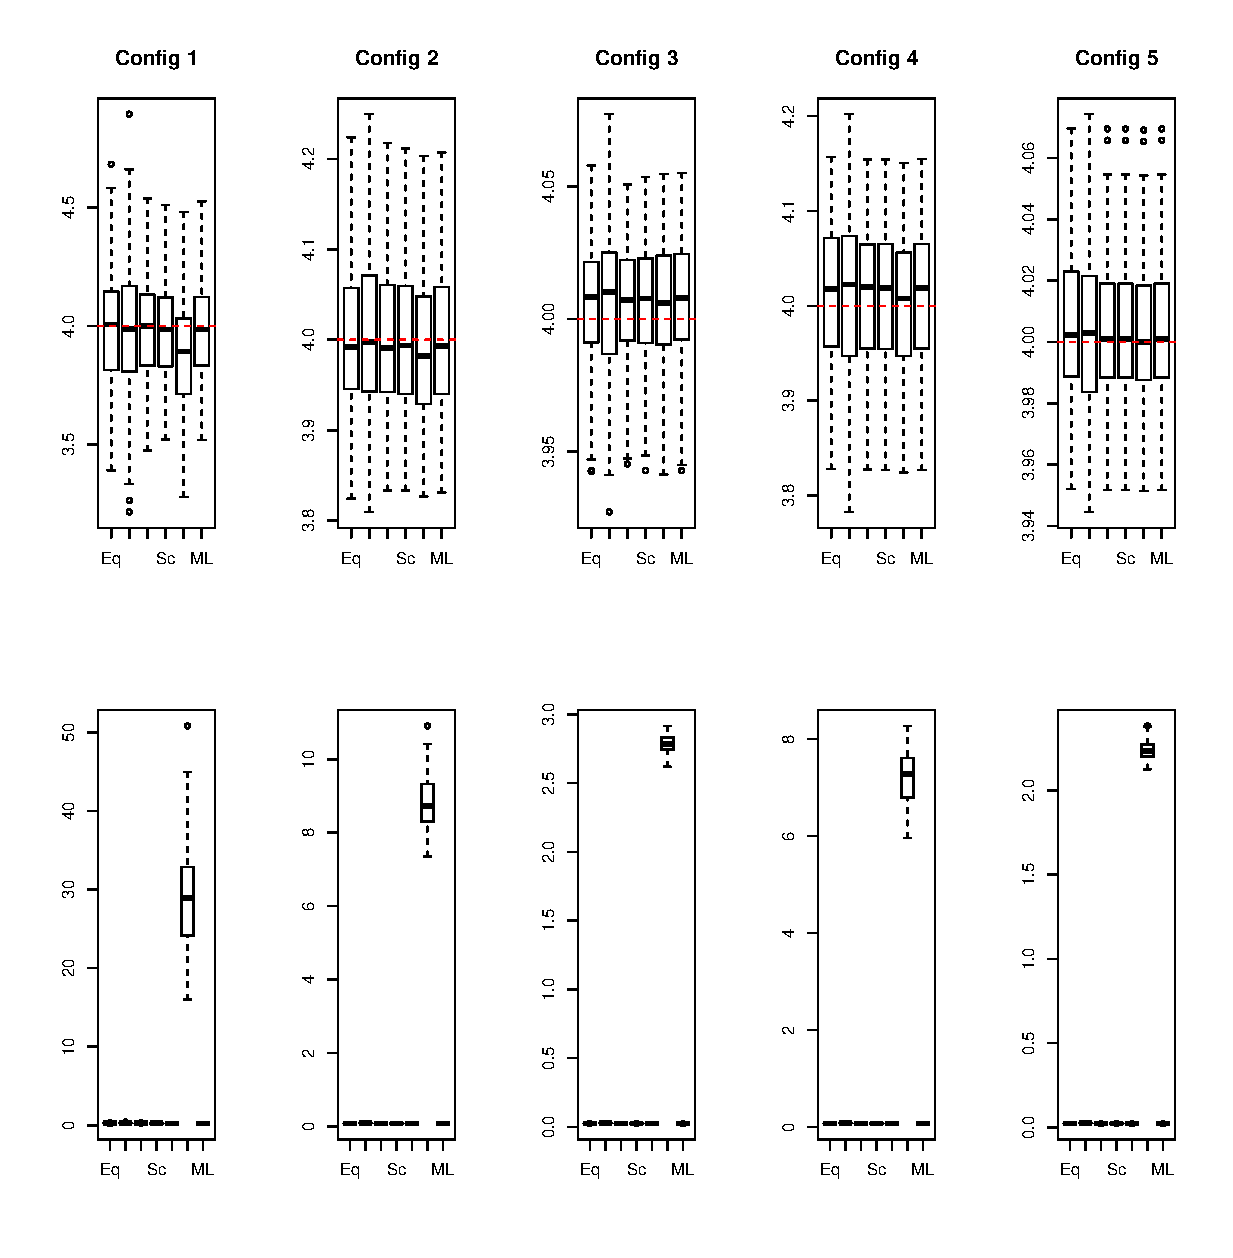
\includegraphics[width=\textwidth]{fig_sigma2.eps}
\caption{\small \linespread{1.1}  Second simulation study. Estimates for $\sigma^2$ (first row) and standard errors (second row).} \label{fig_sigma2}
\end{figure}

\begin{table}[ht]
\centering
\caption{\small \linespread{1.1} Second simulation study. Computation time (in seconds) using closed-form solutions with different implementation forms, compared to PROC MIXED.}

\vspace*{2mm}
\resizebox{\textwidth}{!}{%
\def\arraystretch{1} 
\begin{tabular}{cccccc}
  \hline\hline
&&\multicolumn{2}{c}{Split by split} & & PROC \\ 
\cline{3-4}
Config.& & without loops &  using loops & Together & MIXED \\ 
  \hline
1& Mean & \textbf{0.00520} & 0.00980 & 0.00640 & 0.34155 \\ 
 & S.D. & (0.00882) & (0.00943) & (0.00823) & (0.17711) \\ 
2  &Mean & \textbf{0.02150} & 0.07340 & 0.05660 & 0.35575 \\ 
  &S.D. & (0.01617) & (0.02006) & (0.09662) & (0.03073) \\ 
3  &Mean & \textbf{0.17980} & 0.73480 & 0.43400 & 0.81783 \\ 
  &S.D. & (0.02292) & (0.05835) & (0.11543) & (0.02582) \\ 
4  &Mean & \textbf{0.00220} & 0.00610 & 0.00360 & 2.58808 \\ 
  &S.D. & (0.00579) & (0.01497) & (0.00689) & (0.40720) \\ 
5  &Mean & 0.04030 & 0.27490 &\textbf{ 0.02130} & 629.58333 \\ 
  &S.D. & (0.01521) & (0.01941) & (0.00872) & (116.09435) \\ 
\hline\hline
\end{tabular}}
\end{table}



\begin{table}[ht]
\centering
\caption{\small \linespread{1.1} Second simulation study. Mean, standard deviation (S.D.) and MSE for CS parameter estimates in 100 replications for configuration 2 using different combination weights comparing with full sample MLE and MI-MLE.}
\label{tab_mi_est}

\vspace*{2mm}

\resizebox{\textwidth}{!}{%
\def\arraystretch{1} \begin{tabular}{rcccccccc} 
  \hline\hline
& & Equal & Prop. & Approx.~sc.\ & Scalar & Approx.~opt. & MI & ML \\ 
  \hline
&Mean & -5.09643E-03 & -2.62061E-03 & -2.62061E-03 & -2.88933E-03 & -2.88933E-03 & -8.04195E-03 & -3.28224E-03 \\ 
$\mu$&  S.D. & (4.85424E-02) & (4.91772E-02) & (4.91772E-02) & (4.68032E-02) & (4.68032E-02) & (6.00662E-02) & (4.71723E-02) \\ 
&  MSE & 2.35877E-03 & 2.40108E-03 & 2.40108E-03 & 2.17698E-03 & 2.17698E-03 & 3.63654E-03 & 2.21375E-03 \\ 
&  Mean & 9.98392E-01 & 9.95216E-01 & 9.95216E-01 & 9.70589E-01 & 9.71627E-01 & 3.51123E-02 & 9.92960E-01 \\ 
$d$&   S.D. & (7.33193E-02 & (7.46946E-02) & (7.46946E-02) & (7.59516E-02) & (7.53362E-02) & (1.83983E-02) & (7.50610E-02) \\ 
&   MSE & 5.32455E-03 & 5.54638E-03 & 5.54638E-03 & 6.57598E-03 & 6.42380E-03 & 9.31343E-01 & 5.62737E-03 \\ 
& Mean & 4.00782E+00 & 4.00791E+00 & 4.00581E+00 & 4.00544E+00 & 3.99400E+00 & 5.32627E+00 & 4.00347E+00 \\ 
$\sigma^2$&   S.D. & (7.66500E-02) & (8.98881E-02) & (7.19708E-02) & (7.13441E-02) & (7.19080E-02) & (1.55770E-01) & (7.56968E-02) \\ 
&  MSE & 5.87763E-03 & 8.06169E-03 & 5.16181E-03 & 5.06871E-03 & 5.15505E-03 & 1.78301E+00 & 5.68472E-03 \\ 
   \hline\hline
\end{tabular}}
\end{table}



\begin{table}[ht]
\caption{\small \linespread{1.1} Second simulation study. Mean and standard deviation (S.D.) for the standard error of CS parameter estimates in 100 replications for configuration 2 using different combination weights comparing with full sample MLE and MI-MLE.}
\label{tab_mi_std}

\vspace*{2mm}

\centering
\resizebox{\textwidth}{!}{%
\def\arraystretch{1} \begin{tabular}{rccccccccc}
  \hline\hline
 & & Equal & Prop. & Approx.~sc. & Scalar & Simple opt. & Proper opt. & MI &ML \\   
  \hline
$\mu$ &Mean & 4.24162E-02 & 4.22766E-02 & 4.22766E-02 & 4.11356E-02 & 4.11356E-02 & 4.12439E-02 & 4.95431E-02 & 4.14004E-02 \\ 
 & S.D. & (1.21548E-03) & (8.59430E-04) & (8.59430E-04) & (9.31222E-04) & (9.31222E-04) & (9.42598E-04) & (7.65032E-03) & (9.11785E-04) \\ 
$d$ & Mean & 1.60545E-01 & 2.02922E-01 & 2.02922E-01 & 1.45623E-01 & 7.47531E-02 & 1.48865E+00 & 9.10211E-02 & 7.54391E-02 \\ 
 &  S.D. & (8.88524E-03) & (1.47416E-02) & (1.47416E-02) & (9.84170E-03) & (3.76197E-03) & (1.29914E-01) & (5.18621E-03) & (3.38044E-03) \\ 
$\sigma^2$ & Mean & 7.99442E-02 & 9.26315E-02 & 7.58626E-02 & 7.54139E-02 & 7.49171E-02 & 8.86450E+00 & 1.64310E-01 & 7.50377E-02 \\ 
 &  S.D. & (1.87358E-03) & (3.14842E-03) & (1.39531E-03) & (1.34244E-03) & (1.33807E-03) & (6.56714E-01) & (2.27104E-02) & (1.42688E-03) \\ 
   \hline\hline
\end{tabular}}
\end{table}



\begin{figure}[t]
\centering
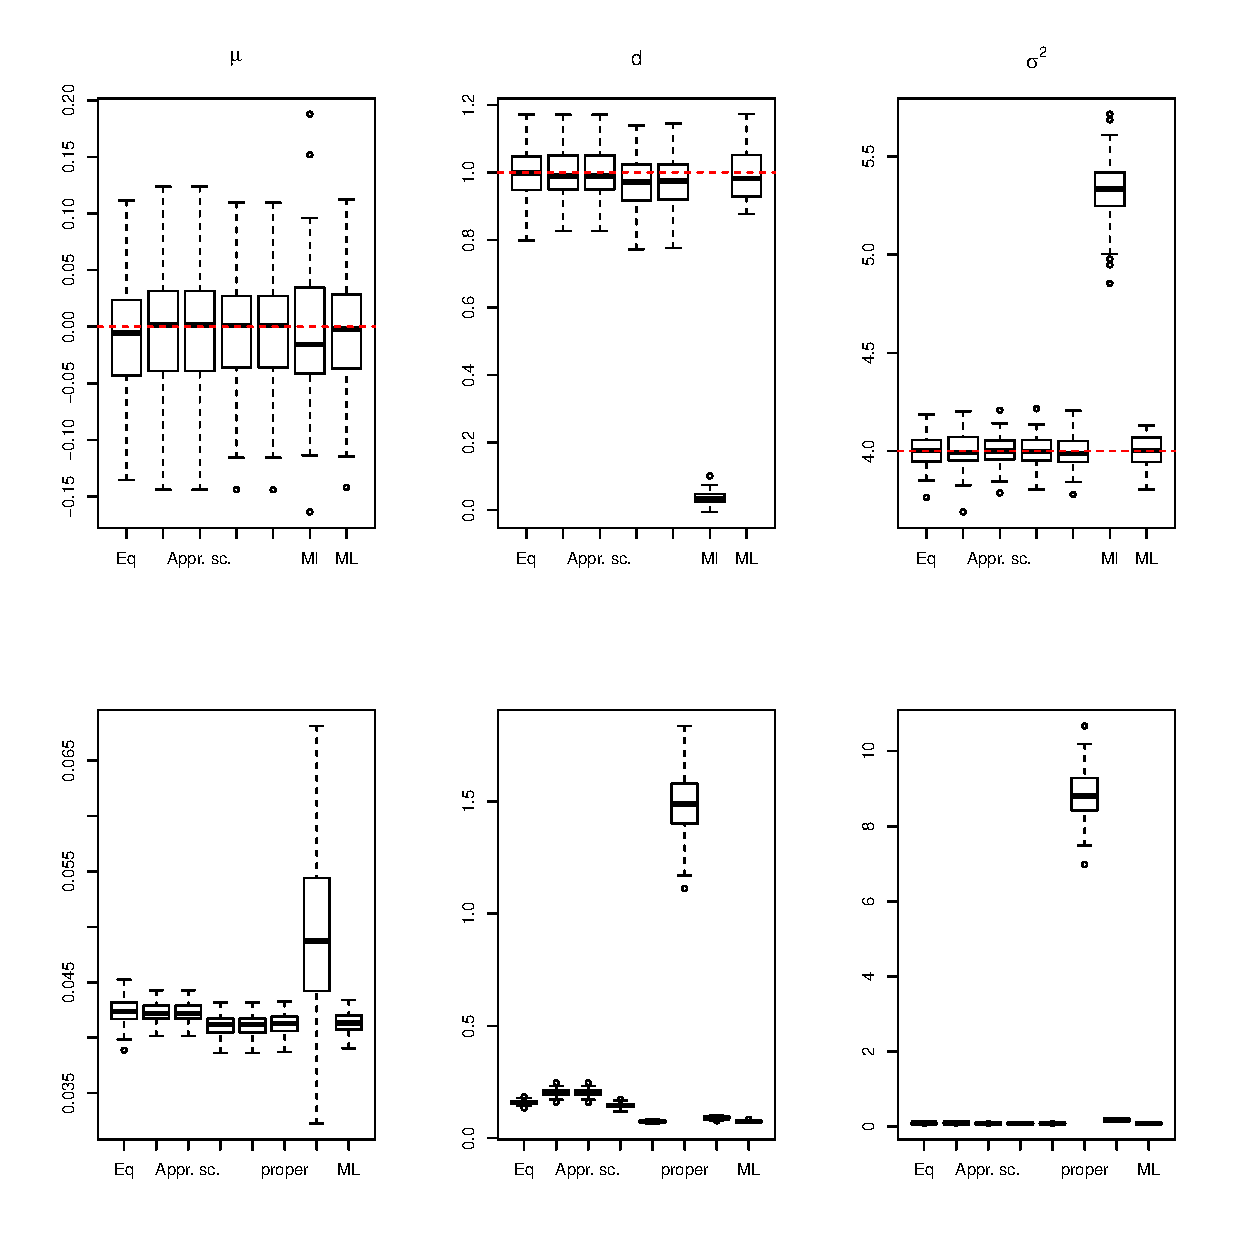
\includegraphics[width=0.9\textwidth]{fig_mi.eps}
\caption{\small \linespread{1.1}  Second simulation study. Estimated CS parameters (first row) and their standard error (second row) using sample splitting, MI-MLE, and MLE.} \label{fig_mi}
\end{figure}

Based on the simulation results, it appears that  using equal weights is not recommended, while using proportional weights produces results comparable with ML. Of course, in case of $\sigma^2$ the approximate scalar weights  work better comparing with ML. An interesting outcome of the simulation is that by keeping the number of clusters of different sizes constant, but allowing the cluster sizes to increase, improves estimation of  $\sigma^2$, while increasing the number of clusters and keeping their sizes constant improves the estimation of  $d$. This is not surprising, because $d$ is the between-cluster variability, which is easier to estimate from a larger number of clusters. This should be seen against the background of relatively small differences anyway. 

The results based on MI are not comparable with sample-splitting results. In particular, the variance component $d$ is underestimated using MI, while $\sigma^2$ is overestimated.  The larger standard errors in this case suggest that the sample-splitting methods use information more efficiently. 

Comparing computation times, the closed-form approaches are the clear winners, further enhanced by smaller standard errors.  Furthermore, it follows that computing the estimates in a semi-parallel fashion, thus avoiding `for' loops within the splits but using then  between splits, is most efficient. Unless the $n_k$'s are very large, computing all  estimates at once is the most efficient. Of course, if the estimates for different splits can be done in parallel (without `for' loops), this is more efficient than estimating them all at once.



%% Ar1
\setcounter{equation}{0}
\section{The balanced conditionally independent model\label{bcim}}

In this case, one imposes the following structure on (\ref{lmmhier}):
\begin{itemize}
\item \Xik\ can be rewritten in terms of a first matrix that imposes structure between clusters (e.g., treatment effect), termed \Aik, and a second one that imposes structure within clusters (e.g., time evolution), $\Tik'=(\Zik',\Qik')'$.
\item The matrices \Aik, \Zik, and \Qik\ are constant among all clusters of size~$n_k$.
\item The matrix $\Sigma_i^{(k)}=\sigma^2I_{n_k}$.
\end{itemize}
This is the general, balanced growth-curve model as studied by \cite{lange1989effect} and \cite{verbeke2007effect}.
\label{setting1est}
Building on their development, we will now derive sufficient statistics and associated maximum likelihood estimators for the parameters in this model. This can be expressed
$$\BY=A(\bfbeta_1,\bfbeta_2)\left(
\begin{array}{c}
Z\\
Q
\end{array}
\right)
 +
BZ
+\beps.
$$
Here, $\BY$ is an $N\times n$ matrix stacking the outcomes of all clusters of size $c$, $A$, $Z$, and $Q$ group the designs mentioned in Section~\ref{defsetting1}, the vectors $\bfbeta_1$ and $\bfbeta_2$ contain the fixed effects, $B$ contains $N$ rows of length $q$, representing the $q$-dimensional random-effects vector, and $\beps$ shares its dimensions with $\BY$.

Now, define $K$ the projection matrix such that $K'K=I_{r-q}$, for an appropriate dimension $r$, and $ZK=0$. Then, set $P=QK$ and consider the projection model:
$$\BY_1\equiv YK=A\bfbeta_2P+\beps K.$$
The variance of a cluster is $\sigma^2I_{r-q}$. Next, define $H$ such that $H'H=I_q$ and $QH=0$. A second projection model emerges:
$$\BY_2\equiv YH=A\bfbeta_1+B+\beps H.$$
The variance of a cluster is $\sigma^2I_q+H'DH$, with $D$ the variance-covariance matrix of the vector of random effects. Importantly, projections $\BY_1\perp \BY_2$.

Conventional algebra leads from these to the following set of sufficient statistics:
\begin{eqnarray}
\label{suffstat1}
T_1&=&(A'A)^{-1}A'\BY_1P'(PP')^{-1},\\
T_2&=&\tr\left\{
\BY_1'\left[I-A(A'A)^{-1}A'\right]\BY_1
\right\},
\\
T_3&=&(A'A)^{-1}A'\BY_2,\\
T_4&=&\BY_2'\left[I-A(A'A)^{-1}A'\right]\BY_2.
\label{suffstat4}
\end{eqnarray}
Sufficient statistics (\ref{suffstat1})--(\ref{suffstat4}) lead to the maximum likelihood estimators:
\begin{eqnarray}
\label{est1}
\widehat{\bfbeta}_1&=&T_1,\\
\widehat{\bfbeta}_2&=&T_3,\\
\widehat{\sigma}^2&=&\frac{1}{N(n-q)}T_2,\\
\widehat{D}&=&\frac{1}{N}T_4-\widehat{\sigma}^2I_q.
\label{est4}
\end{eqnarray}
Note that the estimators for the fixed effects do not involve the variance components.

\setcounter{equation}{0}
\section{Algebraic derivations in the AR(1) case\label{ar1appendix}}

Here, we present more detailed derivations of the key algebraic expressions presented in Sections~\ref{secmodel} and \ref{secestimators}.


\subsection{Some useful expressions}\label{suppexp}

Consider,
\begin{equation}
\label{C}
C =
 \begin{pmatrix}
  1 & \rho & \rho^2 & \rho^3&\ldots \\
   & 1 & \rho & \rho^2 &\ldots \\
   &   & \ddots & \ddots &\ddots  \\
   & & & 1 & \rho\\
   &  & & & 1
 \end{pmatrix},
\end{equation}
then,
\begin{equation}
\label{suppSigma}
\Sigma= \sigma^2 C.
\end{equation}
It can be shown that:
\begin{equation}
\label{det_C}
\mathrm{det}(C)=\left(1-\rho^2 \right)^{n-1}
\end{equation}
The inverse of $C$ can be calculated as follows:
\begin{equation}
\label{inv_C}
C^{-1} =\frac{1}{1-\rho^2}
 \begin{pmatrix}
  1 & -\rho & \ldots & 0 \\
  -\rho & 1+\rho^2 & \ddots & \ldots \\
   &   \ddots & \ddots &\ddots  \\
   &  & 1+\rho^2& -\rho\\
   &   &-\rho& 1
 \end{pmatrix},
\end{equation}
as one may see $C^{-1}$ is a symmetric-tridiagonal matrix with constant diagonal except for the outer entries, and constant first off-diagonal.

Consider:
\begin{equation}
\label{G}
C^{-1}=\frac{1}{1-\rho^2} G.
\end{equation}
Then, by taking the derivative with respect to $\rho$:
\begin{equation}
\label{derivative_c_inv1}
\frac{\partial C^{-1}}{\partial \rho} = \frac{2\rho}{(1-\rho^2)^2}G + \frac{1}{1-\rho^2} H,
\end{equation}
where, $H=\frac{\partial G}{\partial \rho}$ and has the form:
\begin{equation}
\label{H}
H =
 \begin{pmatrix}
  0 & -1 & \ldots & 0 \\
  -1 & 2\rho & \ddots & \ldots \\
  \ddots &   \ddots & \ddots &\ddots  \\
   &\ddots  & 2\rho& -1\\
   0&   &-1& 0
 \end{pmatrix}.
\end{equation}
Also, considering the fact $CC^{-1}=I$, one can derive:
\begin{equation}
\label{derivative_c_inv2}
\frac{\partial C^{-1}}{\partial \rho} = -C^{-1} \frac{\partial C}{\partial \rho} C^{-1}.
\end{equation}

\subsection{The likelihood estimators in a given cluster}

The likelihood function for an $n_k$-dimensional multivariate normal sample of size $c_k$ has the following form:
\begin{equation}
\label{likelihood_general}
L=\prod_{i=1}^{C_k} \frac{1}{|\Sigma|^{1/2} (2\pi)^{n_k/2}}\exp\left\{ -\frac{1}{2} (y_i-\mu_i )' \Sigma^{-1} (y_i-\mu_i) \right\}.
\end{equation}
Therefore, the non-constant terms of the log-likelihood are as follows:
\begin{equation}
\label{log_general}
\ell \propto -\frac{C_k}{2}\ln |\Sigma|. \frac{1}{2}\sum_{i=1}^{C_k} (y_i-\mu_i)' \Sigma^{-1} (y_i-\mu_i),
\end{equation}
which considering (\ref{det_C}) for AR(1):
\begin{equation}
\label{det_simga}
|\Sigma|=\left(\sigma^2 \right)^{n_k} \left(1-\rho^2 \right)^{n_k-1}.
\end{equation}
As a general case, if we consider the mean as linear model with the form $\mu_i=X_i\beta$, one can derive:
\begin{equation}
\label{betahat}
\frac{\partial \ell}{\partial \mu_i}=\Sigma^{-1} \sum_{i=1}^{C_k} (y_i-\mu_i) =0 \Rightarrow \widehat{\beta}=(X'X)^{-1} X'y.
\end{equation}
Now expanding the log-likelihood for $\sigma^2$ and $\rho$, we have:
\begin{equation}
\label{log_likelihood_variance_comp}
\ell \propto -\frac{C_k}{2}n_k \ln\sigma^2 - \frac{C_k}{2} (n_k-1) \ln (1-\rho^2) -\frac{1}{2}\sum_{i=1}^{C_k} (y_i-\mu_i)' \Sigma^{-1} (y_i-\mu_i).
\end{equation}
Considering $\Sigma=\sigma^2 C$ and (\ref{inv_C}), the derivative with respect to $\sigma^2$ is as follows:
\begin{equation}
\label{derivative_sigma_2}
\frac{\partial \ell}{\partial \sigma^2} = -\frac{C_kn_k}{2} \frac{1}{\sigma^2} +\frac{1}{2}\frac{1}{(\sigma^2)^2}\sum_{i=1}^{C_k} (y_i-\mu_i)' C^{-1} (y_i-\mu_i).
\end{equation}
Solving
$\frac{\partial \ell}{\partial \sigma^2} =0$ gives:
\begin{equation}
\label{sigma_2_hat1}
\widehat{\sigma}^2=\frac{1}{C_kn_k}\sum_{i=1}^{C_k} (y_i-\mu_i)' C^{-1} (y_i-\mu_i).
\end{equation}
One may notice that $C^{-1}$ contains the parameter $\rho$.

Taking the derivative of (\ref{log_likelihood_variance_comp}) with respect to $\rho$ gives:
\begin{equation}
\label{derivative_rho}
\frac{\partial \ell}{\partial \rho} =\frac{C_k (n_k-1)}{2}\frac{2\rho}{1-\rho^2} -\frac{1}{\sigma^2}\sum_{i=1}^{C_k} (y_i-\mu_i)' \frac{\partial C^{-1}}{\partial \rho} (y_i-\mu_i).
\end{equation}
Setting $\frac{\partial \ell}{\partial \rho} =0$ gives:
\begin{equation}
\label{rho_hat1}
\widehat{\sigma}^2 \frac{2\widehat{\rho}}{1-\widehat{\rho}^2} = \frac{1}{C_k (n_k-1)} \sum_{i=1}^{C_k} (y_i-\mu_i)' \frac{\partial C^{-1}}{\partial \rho}  (y_i-\mu_i).
\end{equation}
Solving (\ref{sigma_2_hat1}) and (\ref{rho_hat1}) gives $\widehat{\sigma}^2$ and $\widehat{\rho}$. For any ($n_k\times n_k$) matrix $Q$,  $\sum_i (y_i- \mu_i)' Q (y_i-\mu_i)$ 
equals $\mathrm{tr}\left\{ S Q \right\}$,
where $\mathrm{tr}$ denotes the trace of a matrix, and $S=\sum_i (y_i-\mu_i)(y_i-m_i)'$. 
Hence, from (\ref{sigma_2_hat1}), (\ref{rho_hat1}), (\ref{G}), (\ref{derivative_c_inv1}), and (\ref{derivative_c_inv2}), one can write:
\begin{equation}
\label{two_equations}
\begin{cases}
(1-\widehat{\rho}^2) \widehat{\sigma}^2 = \frac{1}{C_k n_k} \mathrm{tr}\{ SG\},\\
(1-\widehat{\rho}^2)\widehat{\sigma}^2 = \frac{1}{C_k n_k}\mathrm{tr}\{SG\} + \frac{1-\widehat{\rho}^2}{2\widehat{\rho}}\frac{1}{C_k(n_k-1)} \frac{1}{C_k(n_k-1} \mathrm{tr}\{SH\}.
\end{cases}
\end{equation}
Set $g=\mathrm{tr}\{SG\}$ and $h=\mathrm{tr}\{SH\}$, it follows that
\begin{equation}
\label{finding_rho}
\frac{g}{n_k} + \frac{1-\widehat{\rho}^2}{2\widehat{\rho}}h =0.
\end{equation}
Given that both $g$ and $h$ are functions of $\rho$ only, $\rho$ can be estimated using ($\ref{finding_rho}$). Given$\rho$, one can use one of equations in (\ref{two_equations}) to estimate $\sigma^2$.

Let us consider some special cases. For $n_k=2$:
\begin{equation*}
\label{n_2_1}
G=
 \begin{pmatrix}
  1 & -\rho\\
 - \rho & 1
 \end{pmatrix},\qquad H=
  \begin{pmatrix}
  0 & -1\\
  -1 & 0
 \end{pmatrix}.
\end{equation*}
Therefore, $g$ and $h$ can be computed as:
\begin{equation*}
g=\mathrm{tr}\left[ \begin{pmatrix}
S_{11} & S_{12} \\
S_{21} & S_{22}
\end{pmatrix}\begin{pmatrix}
1 & -\rho \\
-\rho & 1
\end{pmatrix} \right ] = S_{11} - 2\rho S_{12} + S_{22}.
\end{equation*}
\begin{equation*}
h=\mathrm{tr}\left[ \begin{pmatrix}
S_{11} & S_{12} \\
S_{21} & S_{22}
\end{pmatrix}\begin{pmatrix}
0 & -1 \\
-1 & 0
\end{pmatrix} \right ] = -2S_{12}.
\end{equation*}
Now using (\ref{finding_rho}):
$$\widehat{\rho}(S_{11}- 2\widehat{\rho}S_{12}+S{22}+(1-\widehat{\rho}^2)(-2S_{12}),$$
which gives:
\begin{equation}
\label{n2_hat_rho}
\widehat{\rho}=\frac{2S_{12}}{S_{11}+S_{22}}.
\end{equation}
Then, using first equation in (\ref{two_equations}):
$$(1-\widehat{\rho}^2)\widehat{\sigma}^2 = \frac{1}{2C_k}(S_{11}-2\widehat{\rho}S_{12} + S_{22}),$$
which gives:
\begin{equation}
\label{n2_hat_sigma2}
\widehat{\sigma}^2=\frac{S_{11}+S{22}}{2C_k}.
\end{equation}
For $n_k=3$:
\[
\begin{aligned}
g&=&\mathrm{tr}\left[ \begin{pmatrix}
S_{11} & S_{12} & S_{13} \\
S_{21} & S_{22} & S_{23}\\
S_{31} & S_{32} & S_{33}
\end{pmatrix}\begin{pmatrix}
1 & -\rho & 0\\
-\rho & 1+\rho^2 -\rho\\
0 & -\rho & 1
\end{pmatrix} \right ] \\ &=& S_{11}+S_{22}+S_{33} -2\rho (S_{12} +S_{23})  + \rho^2 S_{22},\\
h&=&\mathrm{tr}\left[ \begin{pmatrix}
S_{11} & S_{12} & S_{13} \\
S_{21} & S_{22} & S_{23}\\
S_{31} & S_{32} & S_{33}
\end{pmatrix}\begin{pmatrix}
0 & -1 &0 \\
-1 & 2\rho & -1\\
0 & -1 & 0
\end{pmatrix} \right ]\\ &=& -2 (S_{12} +S_{23}) + 2 \rho S_{22}.
\end{aligned}
\]
Let,
\begin{equation*}
\begin{cases}
S=S_{11}+S{22}+S{33}\\
R=S_{12}+S_{23}
\end{cases} \Rightarrow \begin{cases}
g=S+\rho^2 S_{22} - 2\rho R\\
h=-2R + 2\rho S_{22}
\end{cases}
\end{equation*}
Using (\ref{finding_rho}):
\begin{equation}
\label{n3}
2S_{22}\rho^3 - R\rho^2 - (S+3 S_{22})\rho + 3R =0.
\end{equation}
Considering the results for $n_k=2$ and $n_k=3$, one can calculate (\ref{finding_rho}) for the general case $n_k=n$ as follows.
\begin{equation}
\label{nk_n_rho}
(n-1) \tilde{S} \rho^3 - (n-2) R \rho^2 - (n\tilde{S}+S)\rho + nR=0
\end{equation}
with:
\begin{equation*}
\begin{cases}
S=S_{11}+\ldots+S_{nn},\\
\tilde{S}=S_{22}+\ldots+S_{n-1,n-1},\\
R=S_{12}+S_{23}+\ldots+S_{n-1,n}.
\end{cases}
\end{equation*}
Then using (\ref{two_equations}):
\begin{equation}
\label{nk_n_sigma2}
\widehat{\sigma}^2=\frac{1}{C_n}\frac{1}{(1-\widehat{\rho}^2)} (S+\widehat{\rho}^2 \tilde{S} - 2\widehat{\rho} R).
\end{equation}
For $n_k>2$,  (\ref{nk_n_rho}) is a third-degree polynomial. One can show that  this equation has only one root in $[-1,1]$.

\begin{proof}
Consider:
\begin{equation*}
\begin{aligned}
 f(\rho) &= (n-1)\tilde{S}\rho^3 - (n-2) R \rho^2 - (n\tilde{S}+S)\rho + nR\\
 f'(\rho) &= 3(n-1)\tilde{S}\rho^2 - 2(n-2) R\rho - (n\tilde{S}+S)\\
  f''(\rho) &= 6(n-1)\tilde{S}\rho - 2(n-2) R
\end{aligned}
\end{equation*}
The discriminant of $f'(\rho)$ is as follows:
\begin{equation*}
\Delta_{f'(\rho)}=(n-2)^2 R^2 + 3 (n\tilde{S}+S)(n-1) \tilde{S}\geq 0.
\end{equation*}
Therefore $f'(\rho)$ has no root and hence $f(\rho)$ is monotone. One may see $f'(0)\leq 0$, therefore, $f(\rho)$ is a monotonically decreasing function (I). One can show $f(1)\leq 0$ and $f(-1)\geq 0$ (II). Considering (I) and (II) together, one may conclude $f(\rho)$ must necessarily cross the horizontal line only once between $[-1,1]$.
\end{proof}
This shows the unique $\widehat{\rho}$ can be easily estimated solving (\ref{nk_n_rho})  using Cardano's formula \citep{Cardano}.


\subsection{Hessians, covariance matrices, and optimal weights}

Given the MLEs for the AR(1) covariance structure,  the Hessians and covariance matrices of the MLEs can be derived. Following the general results obtained about optimal weights, they can be used to compute the exact optimal weights in the case of the AR(1) structure. As mean and variance parameters are orthogonal in the normal case, we can consider the second derivative for fixed effects and variance components separately.

\subsubsection{Second derivative with respect to fixed effects}
As $$\frac{\partial \ell}{\partial \beta}=\sum_{i=1}^{C_k} X'_i\ \Sigma^{-1} (y_i-\mu_i),$$
we have:
\begin{equation*}
\begin{aligned}
\mathrm{E}\left[\frac{\partial \ell}{\partial \beta} \left( \frac{\partial \ell}{\partial \beta}\right)' \right] & = \sum_{i=1}^{C_k} X'_i \Sigma^{-1} \mathrm{E}(y_i-\mu_i)(y_i-\mu_i)' \Sigma^{-1}X_i \\
&= \sum_{i=1}^{C_k} X'_i \Sigma^{-1} X_i.
\end{aligned}
\end{equation*}
For the special case of just an intercept $X_i=\mathbf{1}$:
\begin{multline}
\label{var_mu}
\mathrm{E}\left[\frac{\partial \ell}{\partial \beta} \left( \frac{\partial \ell}{\partial \beta}\right)' \right]= \sum_{i=1}^{C_k} \mathbf{1}' \Sigma^{-1} \mathbf{1}= \\ \frac{C_k}{\sigma^2 (1-\rho^2)}\left[(n_k-2)\rho^2 - 2(n_k-1)\rho +n_k \right].
\end{multline}
Therefore, the variance for $\widehat{\mu}$ can be computed as inverse of (\ref{var_mu}).
\subsubsection{Second derivative with respect to variance components}
To calculate the derivatives with respect to variance components rather than
$\frac{\partial C^{-1}}{\partial \rho}$, we need $K=\frac{\partial C^{-1}}{\partial \rho^2}$. Using these derivatives:
\begin{equation}
\label{useful_deriv}
\begin{cases}
\frac{\partial}{\partial \rho} 2\left(\frac{\rho}{1-\rho^2} \right)= 2\frac{1+\rho^2}{(1-\rho^2)^2},\\
\frac{\partial}{\partial \rho} \frac{\rho}{(1-\rho^2)^2}=\frac{1+3\rho^2}{(1-\rho^2)^3},\\
\frac{\partial}{\partial \rho} \frac{1+\rho^2}{(1-\rho^2)^2} = \frac{2\rho(3+\rho^2)}{(1-\rho^2)^3}.
\end{cases}
\end{equation}
it follows that
\begin{multline}
\label{K}
\frac{\partial C^{-1}}{\partial \rho^2} = K =  \frac{1}{(1-\rho^2)^3} \\
\begin{pmatrix}
2(1+3\rho^2) & -2\rho(3+\rho^2) &   & 0\\
-2\rho(3+\rho^2) & 4(1+3\rho^2) & \ddots &  \ddots\\
 & \ddots & \ddots  & \ddots\\
 0&  &  -2\rho(3+\rho^2) & 2(1+3\rho^2).
\end{pmatrix}
\end{multline}
The second-derivatives are:
\begin{equation}
\label{second_deriv_variance_comp}
\begin{cases}
\frac{\partial^2 \ell}{\partial (\sigma^2)^2} = \frac{C_kn_k}{2}\frac{1}{(\sigma^2)^2}- \frac{1}{(\sigma^2)^3}\sum_{i=1}^{C_k} (y_i-\mu_i)' C^{-1} (y_i-\mu_i),\\
\frac{\partial^2 \ell}{\partial \rho^2} = \frac{C_k(n_k-1)(1+\rho^2)}{(1-\rho^2)^2}-\frac{1}{2\sigma^2}\sum_{i=1}^{C_k} (y_i-\mu_i)' K (y_i-\mu_i),\\
\frac{\partial^2 \ell}{\partial \rho \partial \sigma^2} =\frac{1}{2(\sigma^2)^2}\sum_{i=1}^{C_k} (y_i-\mu_i)'\frac{\partial C^{-1}}{\partial \rho} (y_i-\mu_i).
\end{cases}
\end{equation}
To construct the expected Hessian and covariance matrix, one needs to find the expectations of the expressions in (\ref{second_deriv_variance_comp}).
\begin{equation}
\label{expectation_second_deriv_seigma2}
\mathrm{E}\left(\frac{\partial^2 \ell}{\partial (\sigma^2)^2} \right)= -\frac{C_kn_k}{2}\frac{1}{(\sigma^2)^2}.
\end{equation}
This follows from the fact that: $$\mathrm{E}\left(\sum_{i=1}^ {C_k}  (y_i-\mu_i)' C^{-1} (y_i-\mu_i) \right)=C_k \mathrm{tr}\left\{\mathrm{E}\left[(y_i-\mu_i)'(y_i-\mu_i) \right ] C^{-1}\right\},$$ and $\mathrm{E}\left[(y_i-\mu_i)(y_i-\mu_i)'\right]=\sigma^2 C$.

For the second derivative with respect to $\rho$:
\begin{equation}
\label{expectation_second_deriv_rho1}
\mathrm{E}\left[\frac{\partial^2\ell}{\partial \rho^2} \right]=\frac{C_k(n_k-1)(1+\rho^2)}{(1-\rho^2)^2}-\frac{C_k}{2}\mathrm{tr}\{KS\}.
\end{equation}
Likewise:
\begin{equation}
\label{expectation_deriv_rho_sigma2_1}
\mathrm{E}\left[\frac{\partial^2 \ell}{\partial \rho \partial \sigma^2} \right]=\frac{C_k}{2\sigma^2}\mathrm{tr}\left\{C \frac{\partial C^{-1}}{\partial \rho} \right\}.
\end{equation}
Substituting for $\mathrm{tr}\{KS\}$ and $\mathrm{tr}\left\{C \frac{\partial C^{-1}}{\partial \rho} \right\}$ we get:
\begin{equation}
\label{expectation_deriv_rho_sigma2}
\mathrm{E}\left[\frac{\partial^2 \ell}{\partial \rho \partial \sigma^2} \right]=\frac{C_k(n_k-1)}{\sigma^2}\frac{\rho}{1-\rho^2}.
\end{equation}
\begin{equation}
\label{expectation_second_deriv_rho}
\mathrm{E}\left[\frac{\partial^2\ell}{\partial \rho^2} \right]=-C_k(n_k-1)\frac{1+\rho^2}{(1-\rho^2)^2}.
\end{equation}
Using (\ref{expectation_second_deriv_seigma2}), (\ref{expectation_deriv_rho_sigma2}), and (\ref{expectation_second_deriv_rho}) one obtains the $2\times 2$ Hessian matrix as follows:
\begin{equation}
\label{Hessian}
H=-C_k
\begin{pmatrix}
\frac{n_k}{2(\sigma^2)^2} & -\frac{n_k-1}{\sigma^2} \frac{\rho}{1-\rho^2}\\
-\frac{n_k-1}{\sigma^2} \frac{\rho}{1-\rho^2} & (n_k-1)\frac{1+\rho^2}{(1-\rho^2)^2}
\end{pmatrix}.
\end{equation}
The determinant of the Hessian in (\ref{Hessian}) is as follows:
\begin{equation}
\label{det_hessian}
\mathrm{det}(H)=\frac{C_k^2(n_k-1)(n_k-(n_k-2)\rho^2)}{2(\sigma^2)^2 (1-\rho^2)^2}.
\end{equation}
So,
\begin{multline}
\label{Covariance_biased}
-H^{-1}=\\ \frac{1}{C_k(n_k-(n_k-2)\rho^2)} \begin{pmatrix}
2(\sigma^2)^2 (1+\rho^2) & 2\rho \sigma^2 (1-\rho^2)\\
2\rho \sigma^2 (1-\rho^2) & \frac{n_k}{n_k-1} (1-\rho^2)^2
\end{pmatrix}.
\end{multline}
The Hessian for the unbiased estimator differs slightly from its MLE counterpart:
\begin{eqnarray}
\label{tilde_H}
\tilde{H}&=& -C_k \begin{pmatrix}
\frac{n_k-1}{2(\sigma^2)^2} & -\frac{n_k-1}{\sigma^2} \frac{\rho}{1-\rho^2}\\
-\frac{n_k-1}{\sigma^2} \frac{\rho}{1-\rho^2} & (n_k-1)\frac{1+\rho^2}{(1-\rho^2)^2}
\end{pmatrix},\\
\label{det_tilde_H}
\mathrm{det}(\tilde{H})&=&\frac{C_k^2 (n_k-1)^2}{2(\sigma^2)^2 (1-\rho^2)}.
\end{eqnarray}
Therefore,
\begin{multline}
\label{covariance_unbiased}
-\tilde{H}^{-1}=\\ \frac{1}{C_k(n_k-(n_k-2)\rho^2)} \begin{pmatrix}
2(\sigma^2)^2 (1+\rho^2) & 2\rho \sigma^2 (1-\rho^2)\\
2\rho \sigma^2 (1-\rho^2) &  (1-\rho^2)^2
\end{pmatrix}.
\end{multline}
Having the covariance matrix, one may easily find the optimal weights using
\begin{equation}
\label{optimal_weights}
W_{opt.}=\frac{V^{-1}_k}{\sum_{i=1}^{K} V^{-1}_i}
\end{equation}
The variance of an estimator obtained using the optimal weights in (\ref{optimal_weights}) can be calculated as $\left(\sum_{i=1}^{K} V^{-1}_i\right)^{-1}$.

\subsection{Proof of Proposition~\ref{prop1}\label{suppproof}}

\newcommand{\mua}{\widetilde{\mu}_\alpha}

{\bfseries Proof.} Consider an estimator of the form:
\begin{equation}
\widetilde{\mu}_\alpha=\frac{1}{c}\sum_{i=1}^c\sum_{j=1}^n\alpha_jY_{ij},
\end{equation}
for a vector of weights $\bfalpha=(\alpha_1,\dots,\alpha_n)'$. Because the clusters are i.i.d.\ it is evident that the components of $\bfalpha$ do not depend on the cluster index~$i$. Clearly, the requirement that $E(\mua)=\mu$ implies the condition
\begin{equation}
\label{alphasum}
\sum_{j=1}^n\alpha_j=1.
\end{equation}
 An expression of the variance of $\mua$ combined with this requirement produces the objective function:
\begin{equation}
\label{objfunc1}
Q=\sigma^2\left(
\sum_{j=1}^n\alpha_j^2+2\sum_{j<k}\alpha_j\alpha_k\rho^{|j-k|}
\right)
-\lambda\left(
\sum_{j=1}^n\alpha_j-1
\right),
\end{equation}
with $\lambda$ a Lagrange multiplier. Taking the derivative of (\ref{objfunc1}) w.r.t.\ $\bfalpha$ leads to, after rearrangement:
$$\bfalpha=\frac{\lambda}{2\sigma^2}C^{-1}\eenvec.$$
Given that we have an explicit form for $C^{-1}$, it follows that
\begin{equation}
\label{alphatemp}
\bfalpha=\frac{\lambda}{2\sigma^2(1+\rho)}\bfrho^{(1)},
\end{equation}
with $\bfrho^{(1)}=(1,1-\rho,\dots,1-\rho,1)'$.
Combining (\ref{alphatemp}) with constraint (\ref{alphasum}) leads to
$\lambda=2\sigma^2(1+\rho)/[2+(n-2)(1-\rho)]$, hence
$$\alpha=
\frac{1}{[2+(n-2)(1-\rho)]}\bfrho^{(1)},
$$
establishing the MLE. This completes the proof.

\subsection{Optimal weights in case of a general mean structure $X_i^{(k)}\bfbeta$}\label{suppgenmean}

Cluster size specific expressions are:
\begin{equation}
\widehat{\bfbeta_k}= \left( \sum_{i=1}^{c_k} X_{i}^{(k)'}\Sigma_k^{-1}X_{i}^{(k)}\right)^{-1} \left( \sum_{i=1}^{c_k} X_{i}^{(k)'}\Sigma_k^{-1}Y_{i}^{(k)}\right) \label{betagenmean}
\end{equation}
and
\begin{equation}
\mbox{var}(\widehat{\bfbeta_k})=V_k=\left( \sum_{i=1}^{c_k} X_{i}^{(k)'}\Sigma_k^{-1}X_{i}^{(k)}\right)^{-1}.
\end{equation}
The combination ruleis 
\begin{equation}
\tilde{\bfbeta_k}=\sum_{i=1}^K A_k \widehat{\bfbeta_k},
\end{equation}
with
\begin{equation}
V_k^{-1}=\frac{1}{\sigma^2}\sum_{i=1}^{c_k} X_{i}^{(k)'}C_k^{-1}X_{i}^{(k)}
\end{equation}
and $C_k$ is as described in Supplementary Materials~\ref{suppexp}.

The first factor in (\ref{betagenmean}) can be split into three parts:
$$
\begin{aligned}
(1-\rho^2) X_{i}^{(k)'}C_k^{-1}X_{i}^{(k)} &= X_{i}^{(k)'} (1+\rho^2)I_k X_{i}^{(k)} \label{betaffft}\\
&-\rho^2 X_{i}^{(k)'} \begin{pmatrix}
1 & 0 & \hdots & \hdots & 0 \\
0 & 0 & & & \vdots \\
\vdots & & \ddots & & \\
\vdots & & & 0 & 0 \\
0 & \hdots & \hdots & 0 & 1\\
\end{pmatrix} X_{i}^{(k)} \label{betaffst} \\
&-\rho X_{i}^{(k)'} \begin{pmatrix}
0 & 1 & 0 & \hdots & 0 \\
1 & 0 & \ddots & & \vdots \\
0 & \ddots & \ddots & \ddots & 0 \\
\vdots & & \ddots & 0 & 1 \\
0 & \hdots & 0 & 1 & 0 \\
\end{pmatrix} X_{i}^{(k)}.\label{betafftt}
\end{aligned}
$$

(\ref{betaffft}) simplifies to $(1+\rho^2)X_{i}^{(k)'}X_{i}^{(k)}$, while (\ref{betaffst}) equals
\begin{equation}
\scalemath{0.8}{
\rho^2 \begin{pmatrix}
x_{ki11}^2+x_{kin_k1}^2 & x_{ki11}\cdot x_{ki22}+x_{kin_k1}\cdot x_{kin_k2} & \hdots & x_{ki11}\cdot x_{ki1p} + x_{kin_k1}\cdot x_{kin_kp} \\
 & x_{ki12}^2 + x_{kin_k2}^2 & & \\
 & & \ddots & \\
  & & & x_{ki1p}^2 + x_{kin_kp}^2.
\end{pmatrix}.
}
\end{equation}
Defining $\boldsymbol{X}_{i1}^{(k)}=(x_{ki11} \ \hdots \ x_{ki1p})^t$ and $\boldsymbol{X}_{in_k}^{(k)}=(x_{kin_k1} \ \hdots \ x_{kin_kp})^t$, (\ref{betaffst}) equals
\begin{equation}
\rho^2[\boldsymbol{X}_{i1}^{(k)} \ 0 \hdots 0 \ \boldsymbol{X}_{in_k}^{(k)}] X_i^{(k)}.
\end{equation}
For the third term, define $\boldsymbol{X}_{ij}^{(k)-}=(x_{ki2j} \ \hdots \ x_{kin_kj})^t$ and $\boldsymbol{X}_{ij}^{(k)+}=(x_{ki1j} \ \hdots \ x_{kin_{k-1}j})^t$. As a consequence, (\ref{betafftt}) will equal
\begin{equation}
-\rho [X_i^{(k)-'} \cdot X_i^{(k)+}+X_i^{(k)+'} \cdot X_i^{(k)-}].
\end{equation}
In summary:
\begin{equation}
\begin{aligned}
(1-\rho^2) X_{i}^{(k)'}C_k^{-1}X_{i}^{(k)} &= (1+\rho^2)X_{i}^{(k)'}X_{i}^{(k)} \\
&-\rho^2[\boldsymbol{X}_{i1}^{(k)} \ 0 \hdots 0 \ \boldsymbol{X}_{in_k}^{(k)}] X_i^{(k)} \\
&-\rho [X_i^{(k)-'} \cdot X_i^{(k)+}+X_i^{(k)+'} \cdot X_i^{(k)-}] \\
&\overset{\text{notation}}= F_{1k}. \label{betagenmeanff}
\end{aligned}
\end{equation}
The second factor in (\ref{betagenmean}), using the same notations for $Y_i^{(k)}$ as described above, can be rewritten as:
\begin{equation}
\begin{aligned}
(1-\rho^2) X_{i}^{(k)'}C_k^{-1}Y_{i}^{(k)} =& (1+\rho^2)X_{i}^{(k)'}Y_{i}^{(k)} \\
&- \rho^2 \begin{pmatrix}
x_{ki11}\cdot y_{ki1} + x_{kin_k1}\cdot y_{kin_k}  \\
x_{ki12}\cdot y_{ki1} + x_{kin_k2}\cdot y_{kin_k}  \\
\vdots \\
x_{ki1p}\cdot y_{ki1} + x_{kin_kp}\cdot y_{kin_k} \\
\end{pmatrix}  \\
&-\rho [X_i^{(k)-'} \cdot Y_i^{(k)+}+X_i^{(k)+'} \cdot Y_i^{(k)-}]  \\
&\overset{\text{not.}}= F_{2k}.\label{betagenmeansf}
\end{aligned}
\end{equation}
Combining (\ref{betagenmeanff}) and (\ref{betagenmeansf}) the overall estimate equals:
\begin{equation}
\begin{aligned}
\tilde{\bfbeta_k}&=\sum_{i=1}^K A_k \widehat{\bfbeta_k} \\
&=\sum_{i=1}^K \left( \sum_{m=1}^K F_{1m} \right)^{-1} F_{2k}
\end{aligned}
\end{equation}
\subsection{Delta method for the mean estimator}\label{suppdelta}

By plugging in $\rho_k$ and defining $a_k'=c_k[n_k-(n_k-2)\rho_k]$, equation~(\ref{meanweight}) simplifies to
\begin{equation}
\label{meanweight}
a_k=
\frac
{
a_k'
}
{
\sum_{m=1}^K a_m'
}
,
\end{equation}
and (\ref{varmuk})
becomes
\begin{equation}
\mbox{var}(\widehat{\mu}_k)=v_k=\frac{\sigma_k^2(1+\rho_k)}{a_k'}.
\end{equation}
The first derivatives equal
\begin{equation}
\begin{aligned}
\frac{\partial \tilde{\mu}}{\partial\mu_k} &= a_k = \frac{a_k'}{\sum_{m=1}^K a_m'},  \\
\frac{\partial\tilde{\mu}}{\partial\sigma_k^2}&=0,  \\
\frac{\partial\tilde{\mu}}{\partial\rho_k}&=\frac{-c_k(n_k-2)\sum_{m=1}^Ka_m'(\mu_k-\mu_m)}{\left( \sum_{m=1}^K a_m' \right)^2},
\end{aligned}
\end{equation}
and these can be combined using the delta method, resulting in (\ref{deltavareen}):
\[
\begin{aligned}
\mbox{var}(\tilde{\mu})=& \sum_{i=1}^K \frac{a_k^{'2}}{\left( \sum_{k=1}^K a_k' \right)^2} \cdot \frac{\sigma_k^2(1-\rho_k^2)}{a_k'}\\
& + \frac{\sum_{k=1}^K\left[ c_k(n_k-2)\sum_{m=1}^Ka_m'(\mu_k-\mu_m)\right]^2}{\left( \sum_{k=1}^K a_k' \right)^4}\cdot \frac{1-\rho_k^2}{c_k(n_k-1)}.
\end{aligned}
\]


\subsection{Calculating $\widehat{\rho}$ and $\widehat{\sigma}^2$ in R}

In this section, we consider the implementation of the calculations for the variance components via the R packahe {\tt{fastAR1}}. This can be done with a few simple lines of code. For fixed $C_k=C$ and $n_k=n$, and given the data $y$, the function {\tt{est.ar1}} estimates the variance components and provides a plot for the third-degree polynomial in (\ref{nk_n_rho}). This visually underscores that there is only one root in $[-1,1]$. Figure \ref{3rd_poly} shows (\ref{nk_n_rho}) for 10 simulated data sets;  clearly, there is a single root only in $[-1,1]$. For convenience, the R code can be obtained via R package {\tt{fastAR1}}, see Section~\ref{fastar1}. Other functions to find variances and iterated optimal weights are also available.
\begin{figure}[t]
\centering
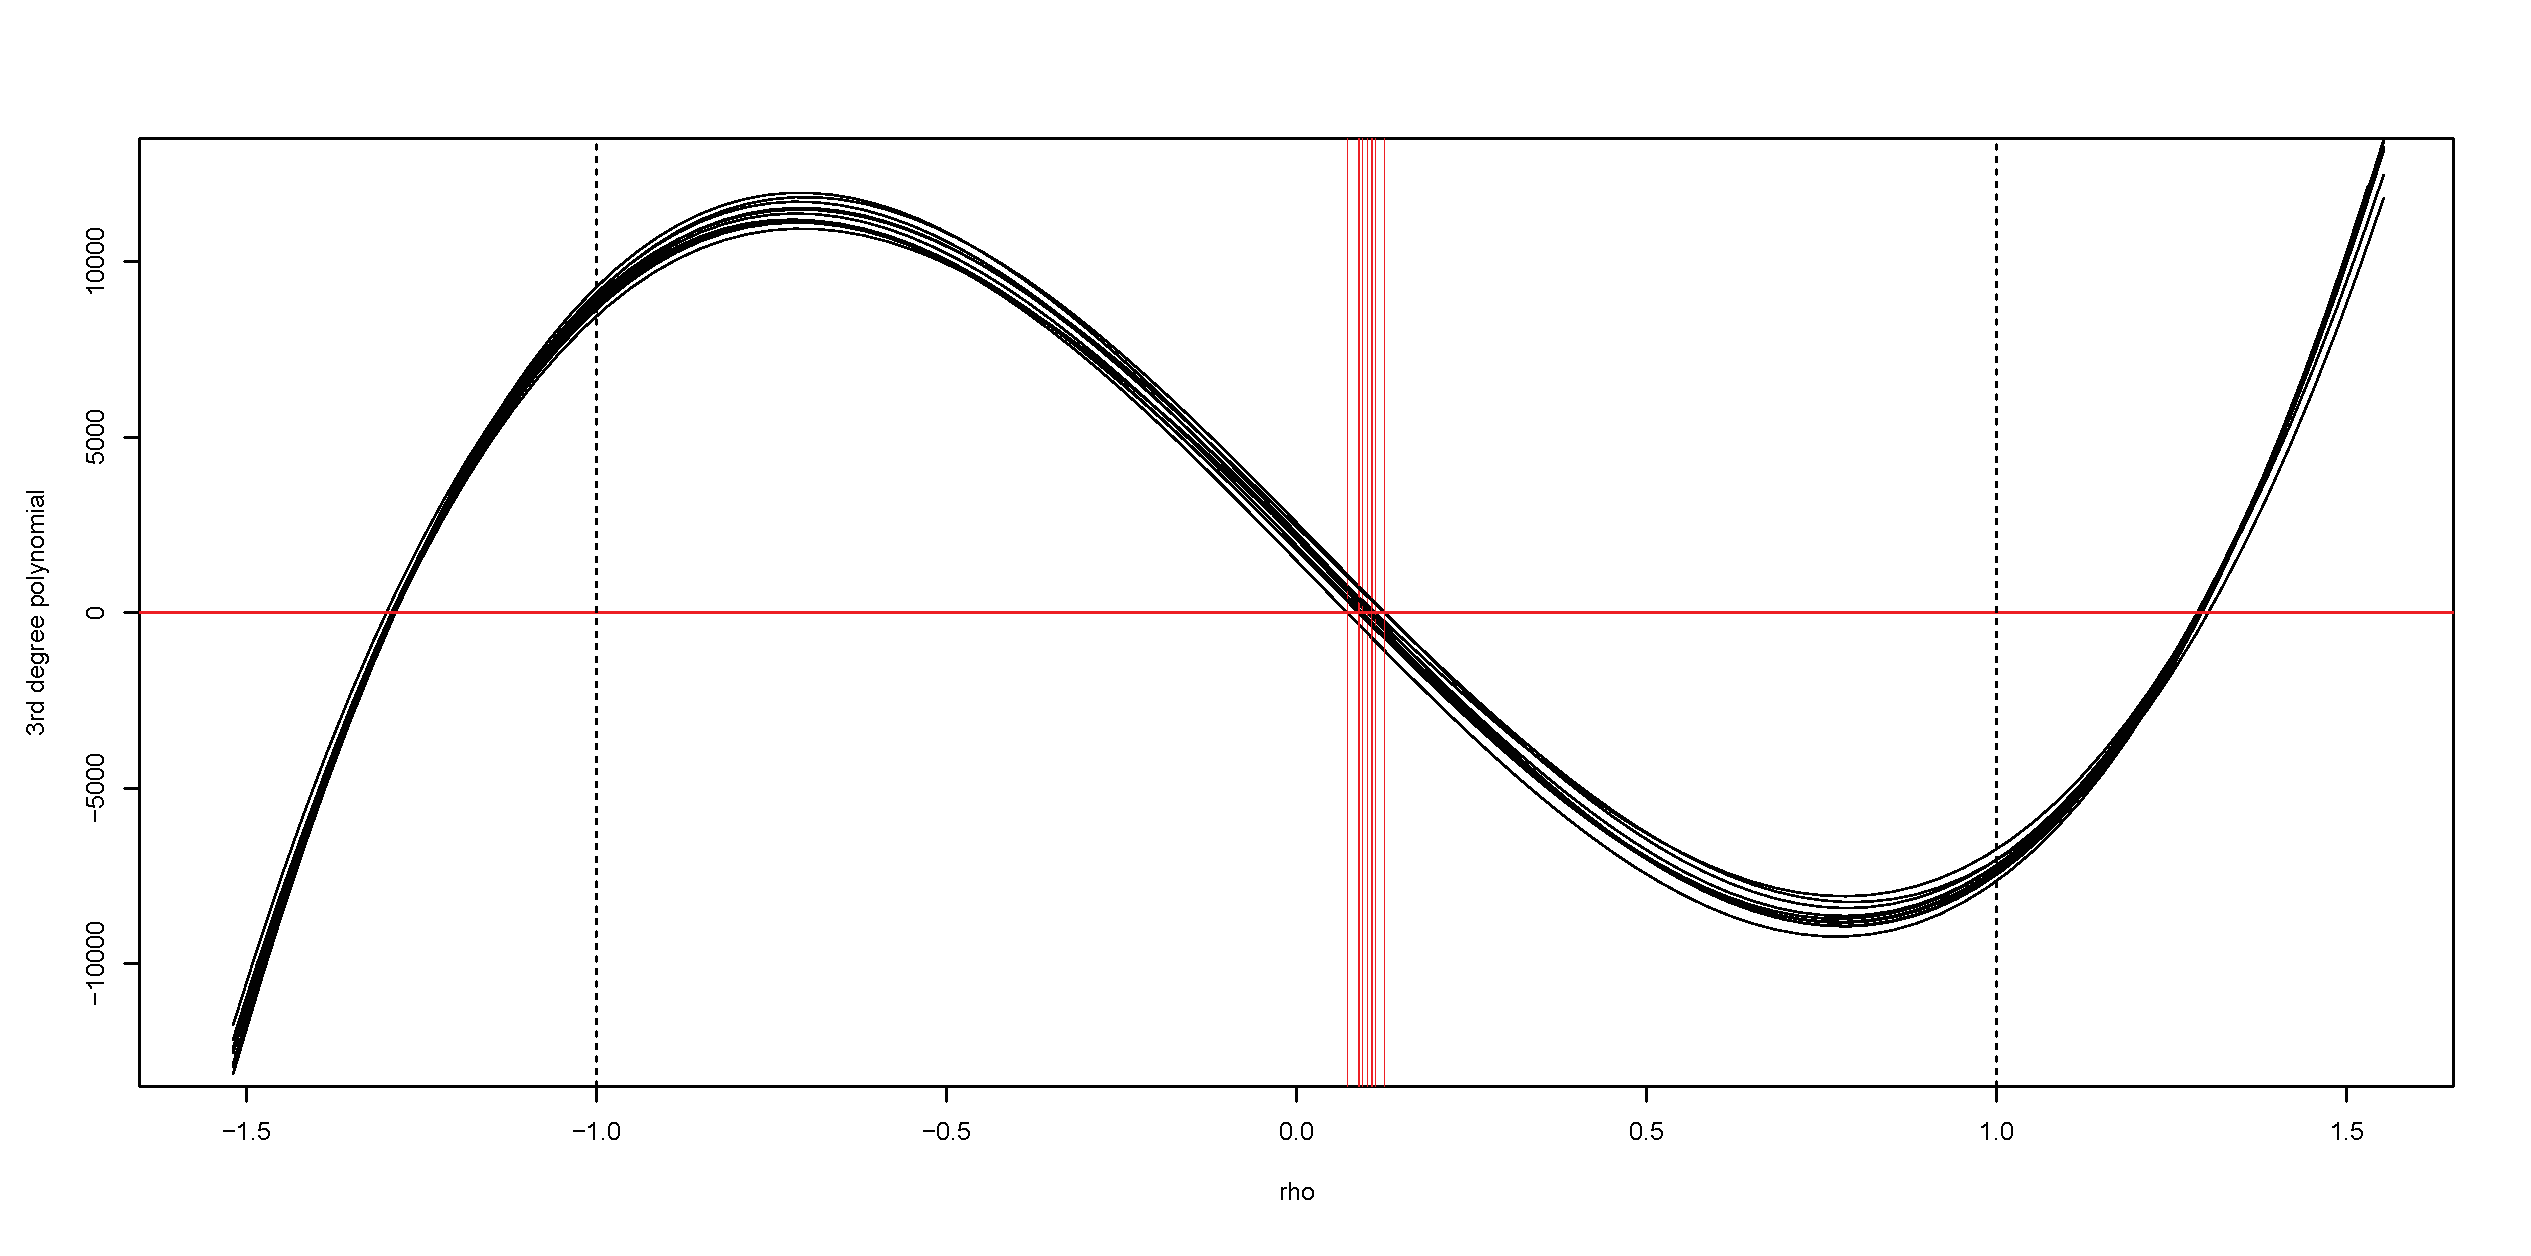
\includegraphics[width=\textwidth]{3rd_poly.eps}
\caption{The third degree polynomial in (\ref{nk_n_rho}) for $10$ different generated data. The red veertical line shows $\widehat{\rho}$.} \label{3rd_poly}
\end{figure}

\setcounter{equation}{0}
\section{Details on additional simulations\label{suppsimul}}

\subsection{Simulations with proportional and size-proportional weights}

Here we consider $C_1=500,  C_2=250 ,C_3=250, C_4= 500$, and $n_1=5,n_2= 10,n_3= 10,n_4=  5$. Parameters are set to $\mu=0$, $\sigma=2$ and $\rho=(0.1,0.5,0.8)$. The data are generated 100 times and the model is fitted using PROC MIXED in SAS (for a single overall intercept). For combining the results from different sub-samples we have used proportional weights and size-proportional weights:
\begin{equation}
\label{weights}
\begin{cases}
\mbox{Prop}=\frac{C_k}{\sum_l C_l}, \\
\mbox{Size.Prop}=\frac{C_kn_k}{\sum_l C_l n_l}.
\end{cases}.
\end{equation}
The results are compared with full likelihood (Table~\ref{table_comp1}). In contrast to the compound-symmetry case, the size-proportional weights show much better results than the proportional weights. Furthermore, the size-proportional weights in the current simulation are identical with the equal weights. The $n_k$'s have a much larger influence in the AR(1) case compared to CS. 
 Figures~\ref{fig_rho1}, \ref{fig_rho2}, and \ref{fig_rho3} make the comparisons easier.
\begin{table}[t]
\centering
\caption{Comparing proportional, size-proportional and iterated optimal weights with full likelihood for AR(1) covariance structure.}
\label{table_comp1}
 \resizebox{\textwidth}{!}{%
\begin{tabular}{clcccccc}
  \hline\hline
 &&$\widehat{\mu}$ & Sd & $\widehat{\rho}$ & Sd & $\widehat{\sigma}^2$ & Sd \\
 \hline
& Prop. & -0.00190 & 0.01615 & 0.10027 & 0.01158 & 1.99642 & 0.03002 \\
  $\rho=0.1$ & Size.Prop.& -0.00207 & 0.01538 & 0.10024 & 0.01080 & 1.99793 & 0.02853 \\
&It.Opt.  & -0.00206 & 0.01538 & 0.10024 & 0.00993 & 1.99792 & 0.02850\\
&ML   & -0.00207 & 0.01538 & 0.10032 & 0.01078 & 1.99793 & 0.02850 \\
  \hline
& Prop.    & -0.00212 & 0.02221 & 0.49966 & 0.00954 & 2.00349 & 0.03652 \\
  $\rho=0.5$ & Size.Prop& -0.00155 & 0.02156 & 0.49955 & 0.00898 & 2.00257 & 0.03494 \\
  &It.Opt.&  -0.00168 & 0.02149  &0.49956 & 0.00826 & 2.00265 & 0.03486\\
 &ML  & -0.00170 & 0.02150 & 0.49986 & 0.00896 & 2.00259 & 0.03488 \\
    \hline
  & Prop. & 0.00195 & 0.02890 & 0.79923 & 0.00549 & 1.99529 & 0.04989 \\
 $\rho=0.8$ &Size.Prop& 0.00234 & 0.02904 & 0.79911 & 0.00530 & 1.99542 & 0.04907 \\
  &It.Opt.& 0.00213 &0.02855& 0.79915& 0.00486&1.99538& 0.04859\\
&ML   & 0.00212 & 0.02855 & 0.79937 & 0.00527 & 1.99519 & 0.04861 \\
   \hline\hline
\end{tabular}}
\end{table}

\begin{figure}[ht!]
\centering
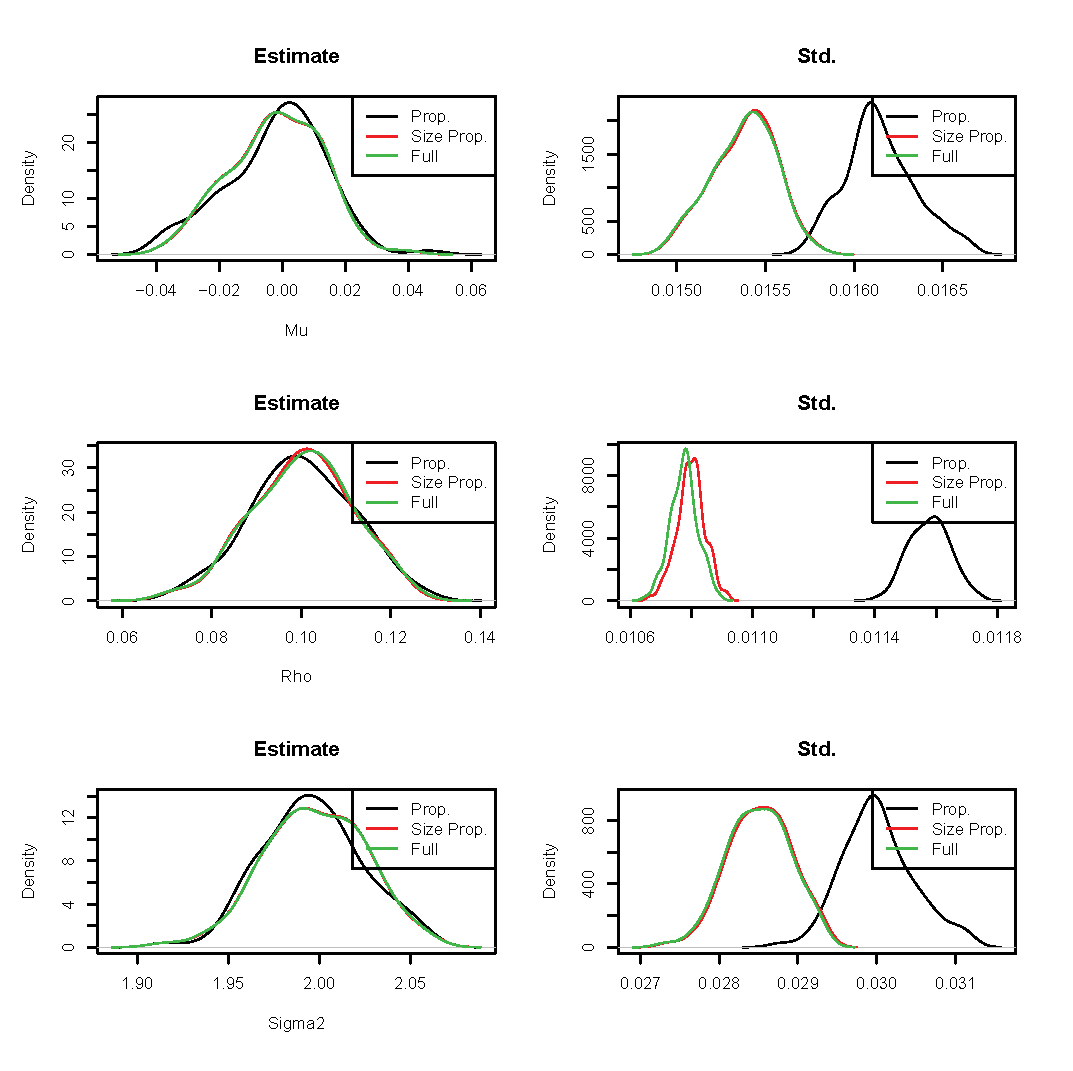
\includegraphics[width=\textwidth]{rho1.eps}
\caption{Comparing proportional and size-proportional weights with full likelihood for $100$ replications with $\mu=0$, $\sigma^2=2$ and $\rho=0.1$.} \label{fig_rho1}
\end{figure}

\begin{figure}[ht!]
\centering
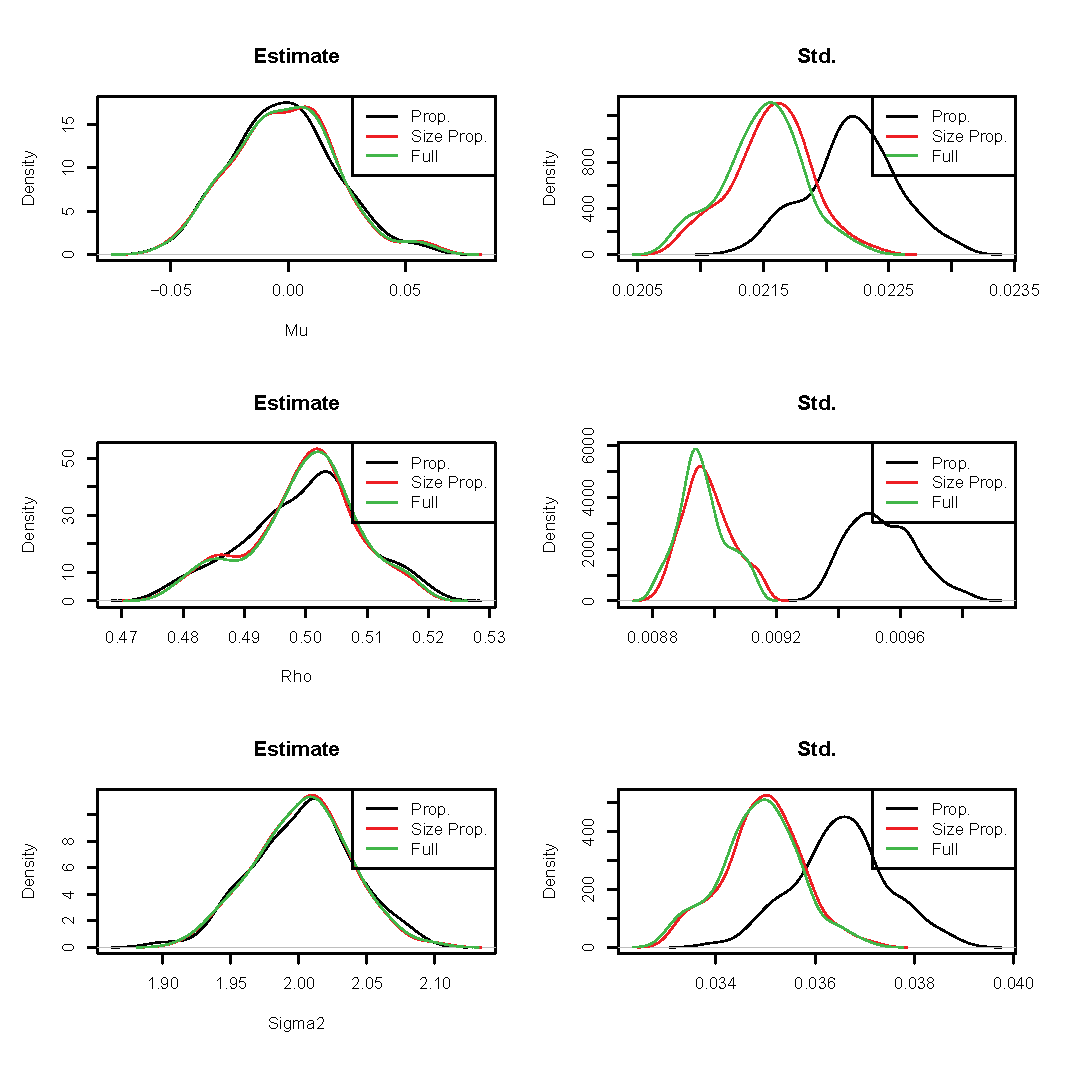
\includegraphics[width=\textwidth]{rho2.eps}
\caption{Comparing proportional and size-proportional weights with full likelihood for $100$ replications with $\mu=0$, $\sigma^2=2$ and $\rho=0.5$.} \label{fig_rho2}
\end{figure}

\begin{figure}[ht!]
\centering
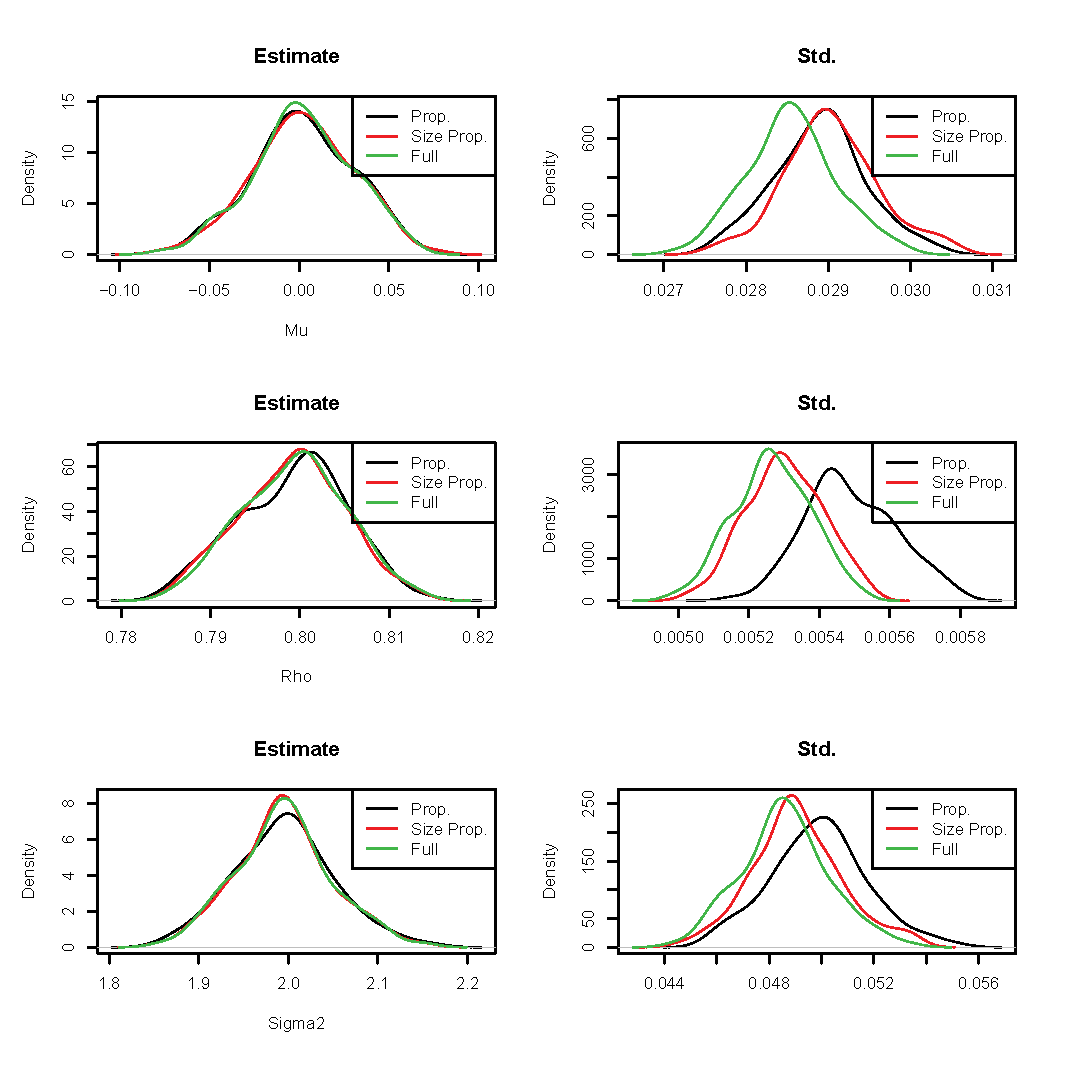
\includegraphics[width=\textwidth]{rho3.eps}
\caption{Comparing proportional and size-proportional weights with full likelihood for $100$ replications with $\mu=0$, $\sigma^2=2$ and $\rho=0.8$.} \label{fig_rho3}
\end{figure}

\subsection{Simulations with proportional and size-proportional weights: $\rho$ near 0/1}

We now present a comparison between proportional and size-proportional weights. We see that,  for $\rho$'s near $1$ (i.e., near CS), size-proportional weights are worse than proportional weights.

We consider $c_1=500$,  $c_2=250$, $c_3=250$, $c_4= 500$, and $n_1=5$, $n_2= 10$, $n_3= 10$, $n_4=  5$. Parameters are set as $\mu=0$, $\sigma=2$ and $\rho\in\{0.01,0.2,0.5,0.8,0.9,0.95,0.99\}$. The data are generated 100 times and the model is fitted using PROC MIXED in SAS (for a single overall intercept). For combining results from different sub-samples we have used proportional weights and size-proportional weights as in (\ref{weights}). The results are compared with full likelihood results.

In Figure~\ref{fig_rho1b}, for $\rho=0.99$ and $0.95$, the size-proportional weights perform  worse than the proportional weights. This is expected, because in this case AR(1) approaches CS. This result is clearer in the left panel of Figure~\ref{fig_rho1b}, where the standard deviations are shown. For $\rho$'s near $1$, the proportional weights are as efficient as  full likelihood, while as $\rho$ moves further from $1$ this would happen for size-proportional weights.

Figure~\ref{fig_rho2b} shows this phenomenon more clearly, as for some selected $\rho$'s ($0.01,0.5,0.95$) the density plot for all $100$ simulated datasets is plotted rather than a  boxplot. The size-proportional weights are better than proportional weights if $\rho$ is not very close to $1$. As soon as $\rho$ becomes $0.95$ or $0.99$, the size-proportional weights become worse.


\begin{figure}[ht!]
\centering
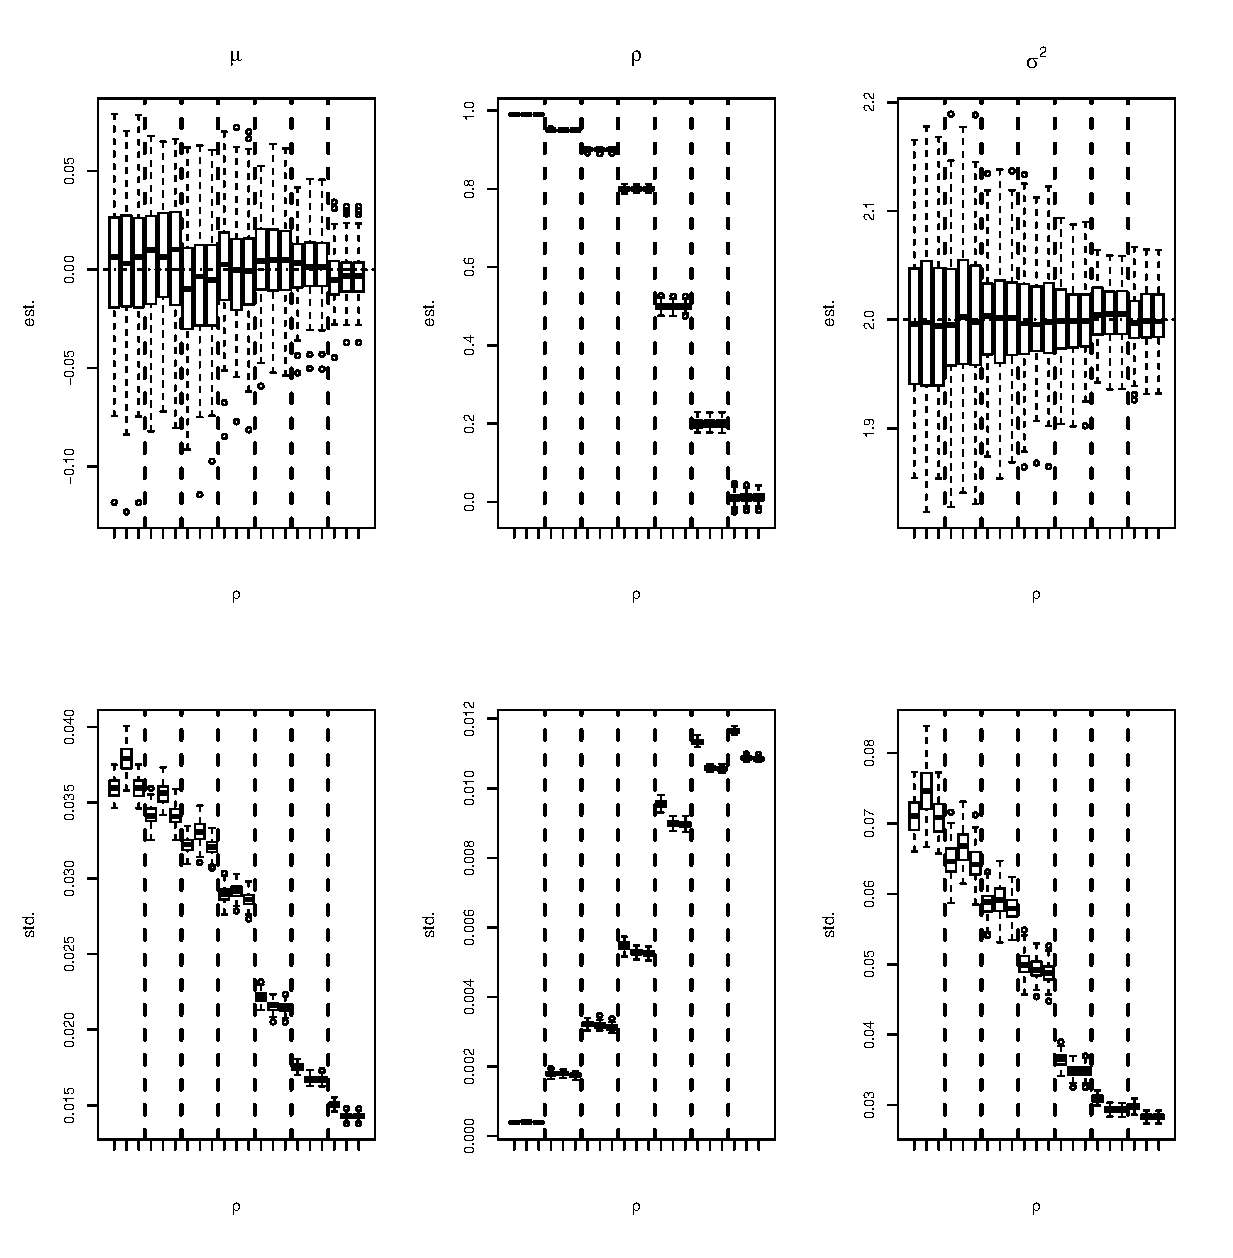
\includegraphics[angle=270]{comp_rho.eps}
\caption[Simulation study. Boxplots comparing proportional and size-proportional weights with full likelihood for $100$ replications with $\mu=0$, $\sigma^2=2$ and $\rho=0.99,0.95,0.9,0.8,0.5,0.2,0.01$]{Simulation study. Boxplots comparing proportional and size-proportional weights with full likelihood for $100$ replications with $\mu=0$, $\sigma^2=2$ and $\rho=0.99,0.95,0.9,0.8,0.5,0.2,0.01$. In every section of the boxplots (which are separated by dashed lines) the first out of three represents the proportional weights, the middle of is size-propotional weights and the one on the right shows the results for the full likelihood. The first row presents the estimates while the second row shows the standard deviations of these estimates.} \label{fig_rho1b}
\end{figure}
\begin{figure}[ht!]
\centering
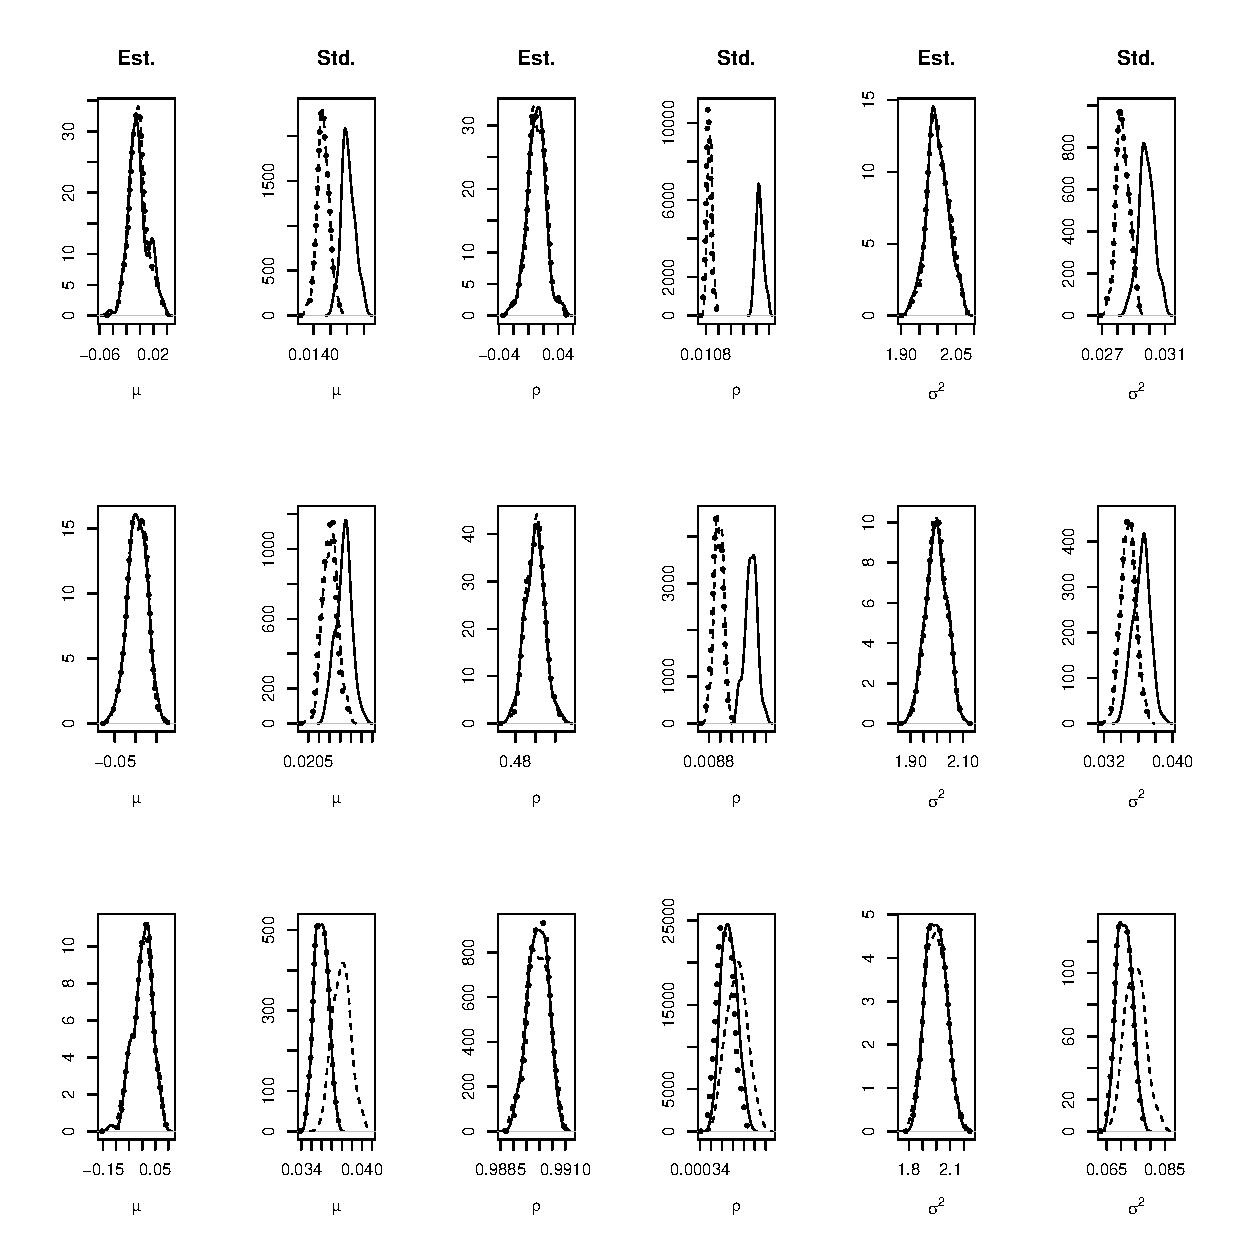
\includegraphics[angle=270]{comp_rho2.eps}
\caption[Simulation study. Comparing proportional, size-proportional and full likelihood results via their empirical density for the 100 replications]{Simulation study. Comparing proportional, size-proportional and full likelihood results via their empirical density for the 100 replications. In all of the figures $\mu=0$ and $\sigma^2=2$. The first row is for $\rho=0.01$, the middle one is for $\rho=0.5$ and last one corresponds to $\rho=0.99$. In each figure the ticker dotted line corresponds to full likelihood, the dashed line is for size-proportional weights and the solid line is for proportional weights.} \label{fig_rho2b}
\end{figure}


\subsection{Simulations with optimal weights}

Given the  covariance matrix of the parameter estimators, finding the optimal weights is straightforward, but in practice the unknown parameters therein need to be estimated.  Here we compare the iterative weights with size-proportional weights and ML. See Figures \ref{fig_rho1_opt}, \ref{fig_rho2_opt}, \ref{fig_rho3_opt}, and Table \ref{table_comp1}.
As expected, the optimal weights lead to estimates very close to the MLE; the difference between them being numerical. 

Size-proportional weights are used as the initial weights to begin the iterative procedure. One interesting outcome of this simulation is that the iterative procedure always converged after just one iteration. This means, iterated optimal weights are just like the approximated optimal weights, but there, instead of using $\widehat{\theta}_k$ from each sub-sample, one may use $\tilde{\theta}$ obtained from all sub-samples using a non-optimal but good weight.

\begin{figure}[ht!]
\centering
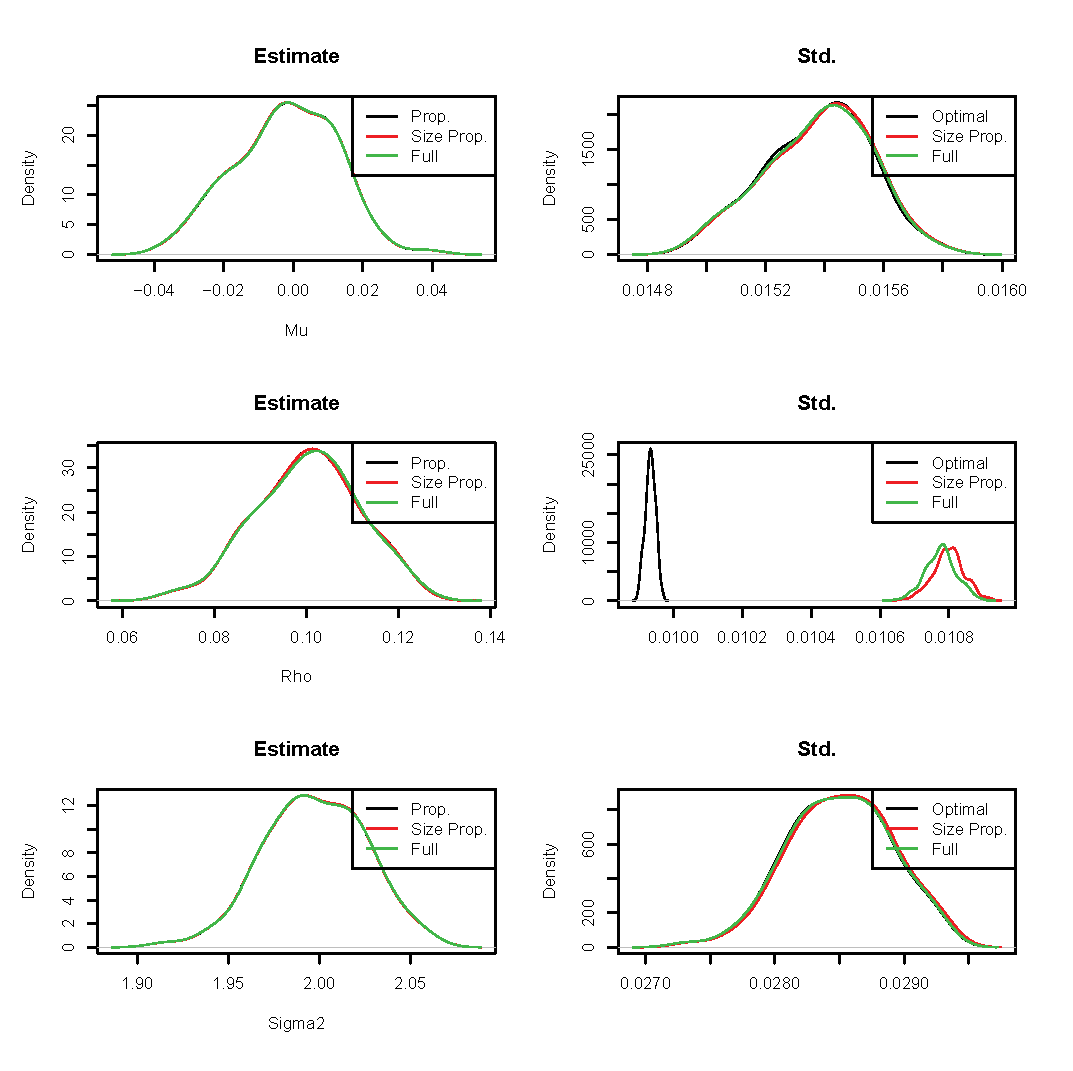
\includegraphics[width=\textwidth]{rho1_opt.eps}
\caption{Comparing iterated optimal and size-proportioanl weights with full likelihood for $100$ replications with $\mu=0$, $\sigma^2=2$ and $\rho=0.1$.} \label{fig_rho1_opt}
\end{figure}

\begin{figure}[ht!]
\centering
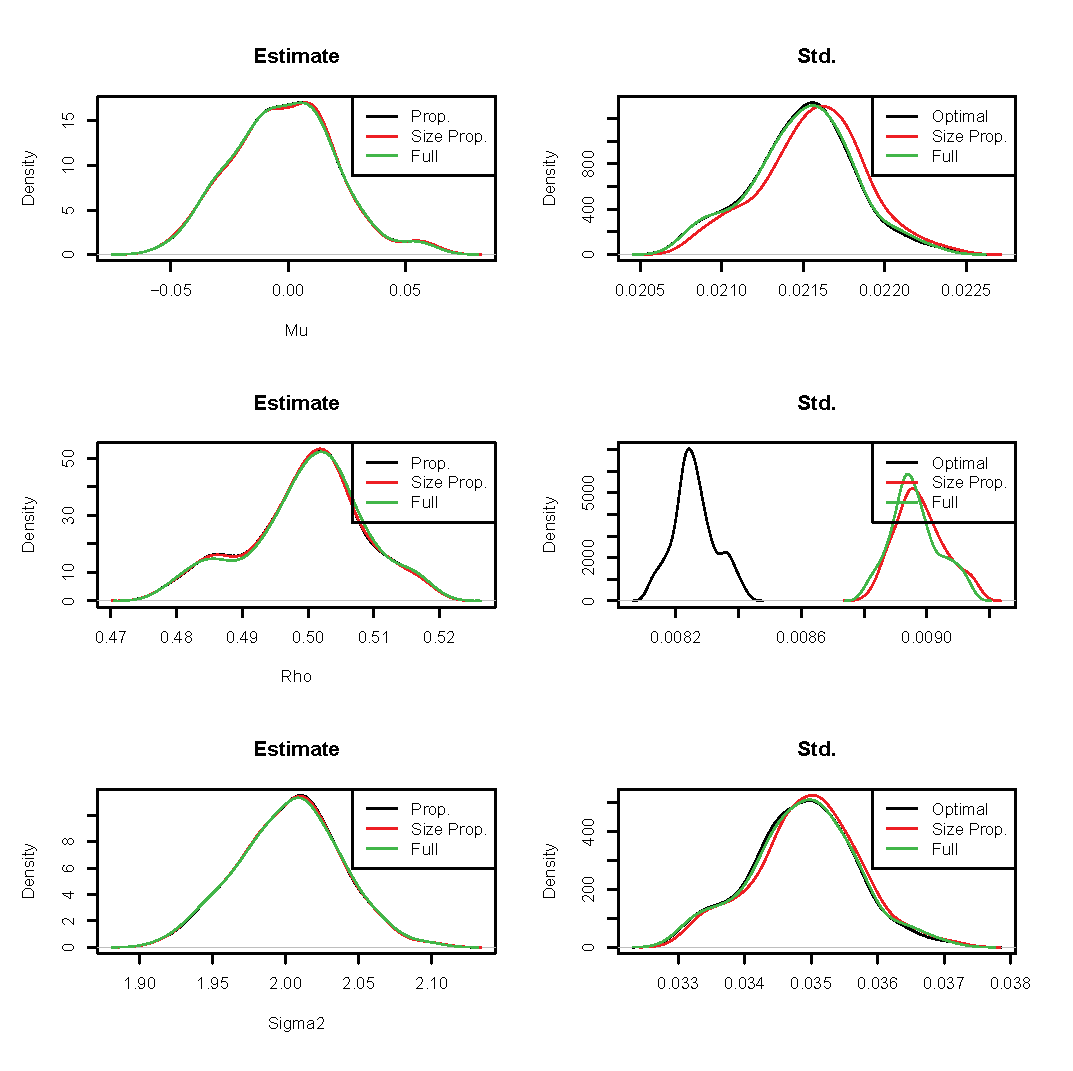
\includegraphics[width=\textwidth]{rho2_opt.eps}
\caption{Comparing iterated optimal and size-proportioanl weights with full likelihood for $100$ replications with $\mu=0$, $\sigma^2=2$ and $\rho=0.5$.} \label{fig_rho2_opt}
\end{figure}

\begin{figure}[ht!]
\centering
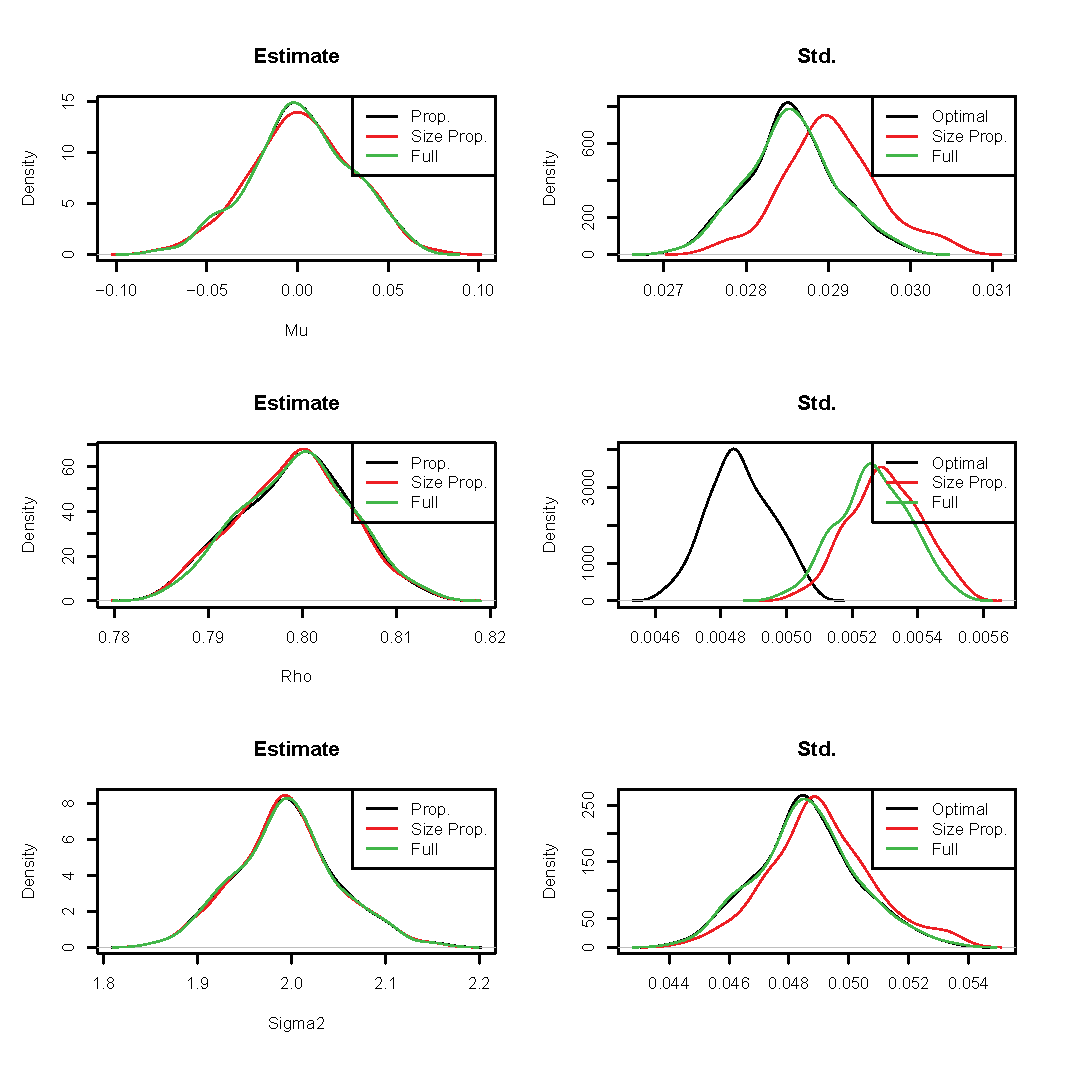
\includegraphics[width=\textwidth]{rho3_opt.eps}
\caption{Comparing iterated optimal and size-proportioanl weights with full likelihood for $100$ replications with $\mu=0$, $\sigma^2=2$ and $\rho=0.8$.} \label{fig_rho3_opt}
\end{figure}


\subsection{Simulations on computation  time}
Here, some summary tables are presented to summarize the results which are already presented via figures earlier. Furthermore, a table and a figure are added to compare computation time for closed form solutions to numerical ones.

In each table the mean of the estimated parameter and its standard deviation using the $100$ replications are given, together with the standard deviation of those 100 numbers (in parentheses). If $\theta$ is the parameter of interest, $\widehat{\theta}$ is its estimate and $\theta_0$ is its real value, then the MSE is computed as follows:
\begin{equation}
\label{MSE}
\mathrm{MSE}(\widehat{\theta})=\frac{1}{100}\sum_{i=1}^{100} (\widehat{\theta}-\theta_0)^2.
\end{equation}
Table~\ref{sim_mu} summarizes the results for $\mu$. The sample splitting estimates are computed using proportional and size-proportional (identical to equal weights in this case) weights. The results using the full sample are also given. The third column in Table~\ref{sim_mu} presents the averaged (over 100 replications) estimated $\mu$ and its standard deviation. The fourth column presents the averaged estimated standard deviation for $\widehat{\mu}$ (over 100 replications) and its standard deviation. The last column shows the MSE computed using (\ref{MSE}) for $\mu_0=1$. Tables~\ref{sim_rho} and \ref{sim_sigma2} shows the same results for $\rho$ and $\sigma^2$ ($\sigma^2_0=2$), respectively.

Table~\ref{comp_time} compares the computation time 
between closed-form and interative methods.  The closed-form solutions are implemented in R and for the numerical methods the MIXED procedure in SAS is used, with error covariance structure set to AR(1).

The data are generated using $n=10$ for all clusters, with $c$ is varying from 100 to 1000000. Therefore, the design is balanced and the point of this comparison is to see how the computation time is reduced in each split.

As one may see in Table~\ref{comp_time} and Figure~\ref{fig_comp_time}, using closed form solutions  significantly reduces the computation time. This means, as well as the computation time reduction due to splitting the data, using closed form solutions within each split the computation time reduction is also huge: for example, for a million clusters, the reduction is from  almost one hour to less than 5 seconds. Figure~\ref{fig_comp_time} shows that computation time using closed form solution changes linearly with the number of clusters, while this will be exponential using an iterative solution.

To assess the effect of the overall size of the dataset, the model is fitted to two concatenated copies of the same set. Computation time results are presented in Table~\ref{comp_time} and Figure~\ref{fig_comp_time}.  The data are generated with $\mu=0$, $\sigma^2=2$, and $\rho=0.25$.
\begin{table}[ht]
\centering
\caption[Simulation study. Estimating $\mu$ and its standard deviation]{Simulation study. Estimating $\mu$ and its standard deviation. The mean (standard deviation) of the $100$ replications are given together with mean squared errors for $\rho=0.01,0.2,0.5,0.8,0.9,0.99$ using proportional and size-proportional weights comparing with the full likelihood results.}
\label{sim_mu}

\vspace*{2mm}
\resizebox{\textwidth}{!} 
{
\begin{tabular}{cllcccc}
\hline\hline
$\rho_0$&method & mean($\widehat{\mu}$) (s.d.)  & mean(s.e.($\widehat{\mu}$)) (s.d.)  & MSE$\times 10^4$ \\
  \hline
  &Prop. & -0.00271 (0.01462) & 0.01503 (0.00020) & 2.19000 \\
0.01  &Size Prop. & -0.00277 (0.01320) & 0.01429 (0.00018) & 1.80172 \\
  &Full & -0.00275 (0.01319) & 0.01428 (0.00018) & 1.79828 \\ \hline
  &Prop. & 0.00158 (0.01677) & 0.01752 (0.00025) & 2.81056 \\
0.2   &Size Prop. & 0.00085 (0.01616) & 0.01673 (0.00021) & 2.59147 \\
  &Full & 0.00090 (0.01615) & 0.01672 (0.00021) & 2.58880 \\ \hline
  &Prop. & 0.00391 (0.02244) & 0.02217 (0.00037) & 5.13770 \\
0.5   &Size Prop. & 0.00397 (0.02191) & 0.02155 (0.00035) & 4.91201 \\
  &Full & 0.00396 (0.02182) & 0.02148 (0.00034) & 4.87038 \\ \hline
  &Prop. & 0.00130 (0.02790) & 0.02894 (0.00050) & 7.72450 \\
0.8   &Size Prop. & -0.00049 (0.02710) & 0.02912 (0.00045) & 7.27464 \\
  &Full & 0.00053 (0.02713) & 0.02862 (0.00045) & 7.29130 \\ \hline
  &Prop. & -0.00828 (0.03006) & 0.03221 (0.00056)&  9.63393 \\
0.9   &Size Prop. & -0.00727 (0.03145) & 0.03306 (0.00070) & 10.3224 \\
  &Full & -0.00803 (0.02998) & 0.03207 (0.00057) & 9.54258 \\ \hline
  &Prop. & 0.00162 (0.03663) & 0.03597 (0.00064) & 13.3123e \\
0.99   &Size Prop. & -0.00007 (0.03930) & 0.03797 (0.00088) & 15.2876 \\
  &Full & 0.00156 (0.03666) & 0.03597 (0.00064) &  13.3305 \\
   \hline
\hline
\end{tabular}}
\end{table}


\begin{table}[ht]
\centering
\caption[Simulation study. Estimating $\rho$ and its standard deviation]{Simulation study. Estimating $\rho$ and its standard deviation. The mean (standard deviation) of the $100$ replications are given together with mean squared errors for $\rho=0.01,0.2,0.5,0.8,0.9,0.99$ using proportional and size-proportional weights comparing with the full likelihood results.}
\label{sim_rho}

\vspace*{2mm}
 \resizebox{\textwidth}{!}{%
\begin{tabular}{lllcccc}
\hline\hline
$\rho_0$&method & mean($\widehat{\rho}$) (s.e.)  & mean(s.e.($\widehat{\rho}$)) (s.e.)  & MSE \\
  \hline
  &Prop. & 0.01077 (0.01237) & 0.01165 (0.00006) &  1.52178e-04 \\
  0.01&Size Prop. & 0.01115 (0.01200) & 0.01087 (0.00004) & 1.43974e-04 \\
  &Full & 0.01123 (0.01203) & 0.01084 (0.00004) & 1.44675e-04 \\  \hline
  &Prop. & 0.19960 (0.01213) & 0.01133 (0.00007) & 1.45806e-04  \\
 0.2 &Size Prop. & 0.19973 (0.01145) & 0.01058 (0.00005) &  1.29974e-04 \\
  &Full& 0.19986 (0.01142) & 0.01056 (0.00005) & 1.29174e-04 \\  \hline
  &Prop. & 0.49956 (0.00963) & 0.00954 (0.00011) & 9.19119e-05 \\
0.5  &Size Prop. & 0.49965 (0.00904) & 0.00898 (0.00008) & 8.11057e-05 \\
  &Full & 0.49990 (0.00904) & 0.00896 (0.00008) & 8.08877e-05 \\  \hline
  &Prop. & 0.79973 (0.00541) & 0.00548 (0.00012) & 2.90660e-05 \\
0.8  &Size Prop & 0.79990 (0.00483) & 0.00529 (0.00009) & 2.31132e-05 \\
  &Full & 0.80018 (0.00489) & 0.00525 (0.00009) &  2.36726e-05 \\  \hline
  &Prop. & 0.90017 (0.00286) & 0.00321 (0.00008) & 8.14862e-06 \\
0.9  &Size Prop. & 0.90013 (0.00297) & 0.00318 (0.00008) & 8.76257e-06 \\
  &Full & 0.90040 (0.00292) & 0.00312 (0.00008) & 8.60114e-06 \\  \hline
  &Prop. & 0.98994 (0.00038) & 0.00039 (0.00001) & 1.45292e-07 \\
0.99  &Size Prop. & 0.98992 (0.00042) & 0.00041 (0.00002) & 1.77848e-07 \\
  &Full & 0.98997 (0.00037) & 0.00039 (0.00001) & 1.37289e-07  \\
   \hline\hline
\end{tabular}}
\end{table}


\begin{table}[ht]
\centering
\caption[Simulation study. Estimating $\sigma^2$ and its standard deviation]{Simulation study. Estimating $\sigma^2$ and its standard deviation. The mean (standard deviation) of the $100$ replications are given together with mean squared errors for $\rho=0.01,0.2,0.5,0.8,0.9,0.99$ using proportional and size-proportional weights comparing with the full likelihood results.}
\label{sim_sigma2}

\vspace*{2mm}
 \resizebox{\textwidth}{!}{%
\begin{tabular}{lllcccc}
\hline\hline
$\rho_0$&method& mean($\widehat{\sigma}^2$) (s.e.)  & mean(s.e.($\widehat{\sigma}^2$)) (s.e.)  & MSE \\
  \hline
  &Prop. & 1.99964 (0.02960) & 0.02981 (0.00049) & 8.67280e-04 \\
0.01  &Size Prop. & 2.00165 (0.02836) & 0.02834 (0.00040) & 7.98842e-04 \\
  &Full & 2.00167 (0.02832) & 0.02832 (0.00040) & 7.97002e-04 \\   \hline
  &Prop. & 2.00581 (0.02907) & 0.03093 (0.00055) & 8.70077e-04  \\
0.2  &Size Prop. & 2.00484 (0.02778) & 0.02936 (0.00044) & 7.87298e-04 \\
  &Full & 2.00473 (0.02772) & 0.02933 (0.00044) & 7.83248e-04 \\   \hline
  &Prop. & 1.99783 (0.03860) & 0.03638 (0.00097) & 1.47960e-03 \\
0.5  &Size Prop. & 1.99890 (0.03747) & 0.03488 (0.00085) & 1.39116e-03 \\
  &Full & 1.99897 (0.03748) & 0.03481 (0.00085) & 1.39152e-03 \\   \hline
  &Prop. & 2.00013 (0.04900) & 0.05002 (0.00166) & 2.37744e-03 \\
0.8  &Size Prop. & 2.00136 (0.04423) & 0.04930 (0.00137) & 1.93881e-03 \\
  &Full & 2.00101 (0.04569) & 0.04880 (0.00142) & 2.06754e-03 \\   \hline
  &Prop. & 2.00122 (0.05767) & 0.05872 (0.00196) & 3.29407e-03 \\
0.9  &Size Prop. & 2.00089 (0.06037) & 0.05915 (0.00230) & 3.60829e-03 \\
  &Full & 2.00115 (0.05876) & 0.05793 (0.00198) &  3.41986e-03 \\   \hline
  &Prop. & 1.99683 (0.06941) & 0.07117 (0.00254) & 4.77911e-03\\
0.99  &Size Prop. & 1.99527 (0.07598) & 0.07484 (0.00344) & 5.73813e-03 \\
  &Full & 1.99641 (0.06940) & 0.07093 (0.00253) & 4.78099e-03 \\
   \hline\hline
\end{tabular}}
\end{table}


\addtolength{\tabcolsep}{-.9mm}

\begin{table}[ht]
\centering
\caption[Simulation study. The computation time]{Simulation study. The computation time for a sample with $n=10$ and $c=$1e+02, 1e+03, 1e+04, 5e+04, 1e+05, 3e+05, 5e+05, 7e+05, 9e+05, 1e+06. The closed form solution is obtained by implementing the results of this paper in R, and the numerical solution is obtained using PROC MIXED in SAS to estimate a repeated measurement model with AR(1) covariance structure.}
\label{comp_time}

\vspace*{2mm}
 \resizebox{\textwidth}{!}{%
\begin{tabular}{lcccccccccc}
  \hline\hline
 time (s) & 1e+02 &1e+03&1e+04& 5e+04& 1e+05& 3e+05 &5e+05 &7e+05& 9e+05 &1e+06\\
   \hline
  Closed form & 0.00 & 0.00 & 0.03 & 0.23 & 0.34 & 1.45 & 2.07 & 3.37 & 4.40 & 4.89 \\
  Numerical & 0.08 & 0.13 & 1.04 & 10.45 & 34.74 & 268.96 & 770.74 & 1611.43 & 2724.31 & 3399.47 \\
   \hline
\hline
\end{tabular}}
\end{table}


\addtolength{\tabcolsep}{.9mm}


\begin{figure}[t]
\centering
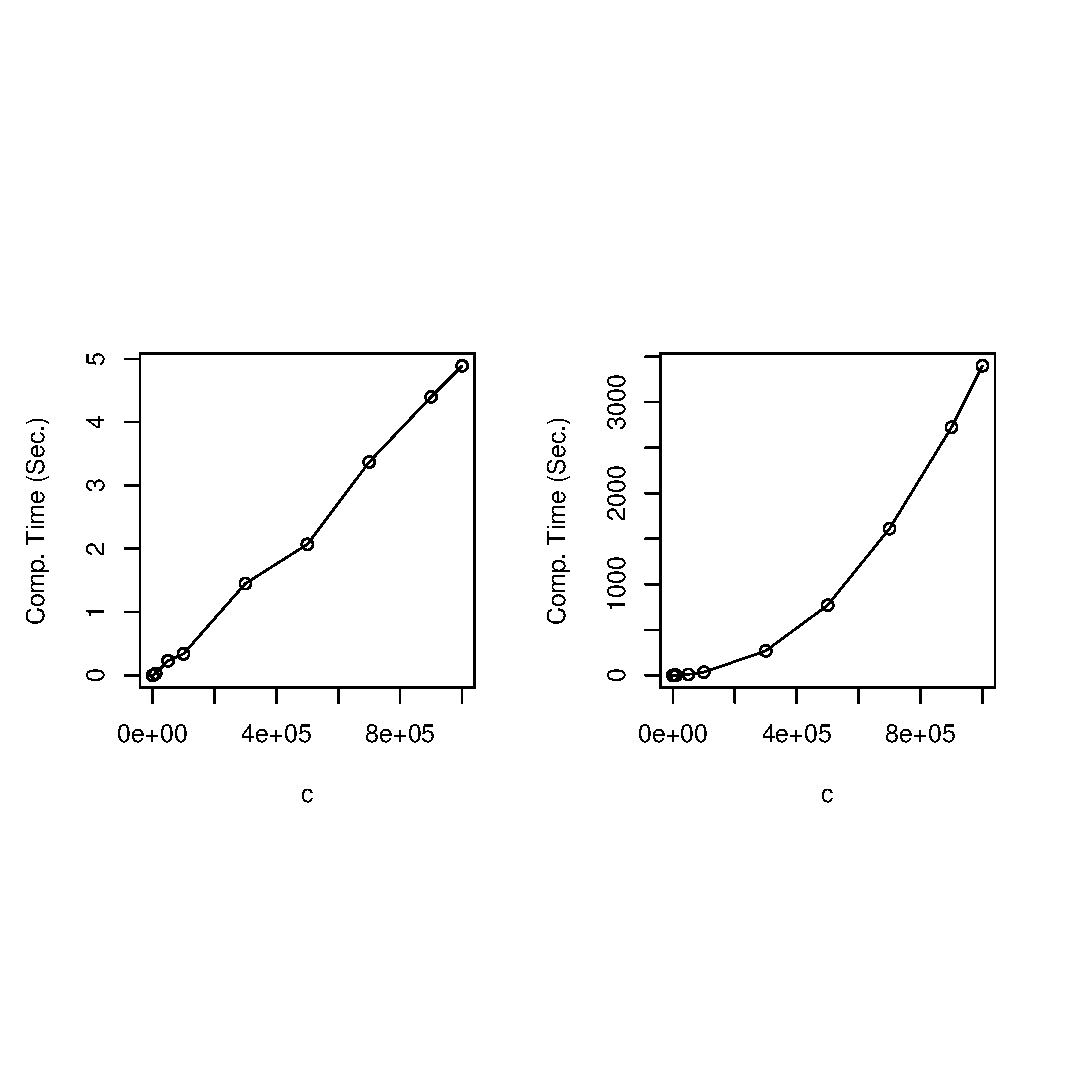
\includegraphics[width=\textwidth, trim= 0cm 4cm 0cm 4cm]{comp_time.eps}
\caption[Simulation study. Comparing computation time using closed form and numerical solutions]{Simulation study. Comparing computation time using closed form (left) and numerical (right) solutions. The horizontal axis shows number of clusters ($c$) and the vertical axis shows the computation time in seconds.} \label{fig_comp_time}
\end{figure}

\setcounter{equation}{0}
\section{Details on PANSS data analysis}\label{suppdata}
\vspace{-3.5mm}
As one may see from Table~\ref{PANSSTab_freq}, by far the majority of the study subjects have complete data and hence belong to the first pattern.

 Figure~\ref{fig_all_first} presents boxplots for the entire set of data, for the subjects from the first pattern only, and for various split samples. 


\begin{table}[ht!]
\centering
\caption{PANSS data. Number of clusters in each trial for each cluster pattern.}
\label{PANSSTab_freq}\vspace*{2mm}
 \resizebox{\textwidth}{!}{%
\begin{tabular}{rcccccccccccccccc}
\hline\hline
 & &&&&&&&&&&  \multicolumn{5}{c}{Trial} &  \\
  \cline{12-16}
$n$ & \multicolumn{10}{c}{Pattern}  & FIN-1 & FRA-3 & INT-2 & INT-3 & INT-7 &Total  \\
  \hline
 &  $\ast$& $\ast$& $\cdot$& $\cdot$& $\cdot$& $\cdot$& $\cdot$& $\cdot$&  $\cdot$&  $\cdot$&  17 & 8 & 71 & 43 & 3 & 142 \\
  2 &  $\ast$& $\cdot$& $\ast$& $\cdot$& $\cdot$& $\cdot$& $\cdot$& $\cdot$&  $\cdot$&  $\cdot$ & 0 & 0 & 2 & 0 & 1 & 3 \\
   &  $\ast$& $\cdot$& $\cdot$& $\cdot$& $\ast$& $\cdot$& $\cdot$& $\cdot$&  $\cdot$&  $\cdot$ & 0 & 0 & 1 & 0 & 0 & 1 \\ \hline
   &  $\ast$& $\ast$& $\ast$& $\cdot$& $\cdot$& $\cdot$& $\cdot$& $\cdot$&  $\cdot$&  $\cdot$ & 8 & 4 & 83 & 41 & 7 & 143 \\
  3 &  $\ast$& $\cdot$& $\ast$& $\cdot$& $\ast$& $\cdot$& $\cdot$& $\cdot$&  $\cdot$&  $\cdot$ & 0 & 0 & 2 & 0 & 0 & 2 \\
   &  $\ast$& $\ast$& $\cdot$& $\cdot$& $\ast$& $\cdot$& $\cdot$& $\cdot$&  $\cdot$&  $\cdot$ & 1 & 0 & 3 & 1 & 0 & 5 \\ \hline
   &  $\ast$& $\ast$& $\ast$& $\cdot$& $\ast$& $\cdot$& $\cdot$& $\cdot$&  $\cdot$&  $\cdot$ & 11 & 0 & 85 & 66 & 5 & 167 \\
   &  $\ast$& $\cdot$& $\ast$& $\cdot$& $\ast$& $\cdot$& $\ast$& $\cdot$&  $\cdot$&  $\cdot$ & 0 & 0 & 1 & 0 & 1 & 2 \\
  4 &  $\ast$& $\cdot$& $\ast$& $\cdot$& $\ast$& $\cdot$& $\cdot$& $\ast$&  $\cdot$&  $\cdot$ & 0 & 0 & 1 & 0 & 0 & 1 \\
   &  $\ast$& $\ast$& $\ast$& $\cdot$& $\cdot$& $\cdot$& $\ast$& $\cdot$&  $\cdot$&  $\cdot$ & 0 & 0 & 3 & 0 & 0 & 3 \\
   &  $\ast$& $\ast$& $\ast$& $\ast$& $\cdot$& $\cdot$& $\cdot$& $\cdot$&  $\cdot$&  $\cdot$ & 0 & 4 & 1 & 0 & 0 & 5 \\
   &  $\ast$& $\ast$& $\cdot$& $\ast$& $\cdot$& $\cdot$& $\ast$& $\cdot$&  $\cdot$&  $\cdot$ & 0 & 1 & 0 & 0 & 0 & 1 \\
  &  $\ast$& $\cdot$& $\ast$& $\cdot$& $\cdot$& $\cdot$& $\ast$& $\ast$&  $\cdot$&  $\cdot$ & 0 & 0 & 0 & 0 & 1 & 1 \\ \hline
   &  $\ast$& $\ast$& $\ast$& $\cdot$& $\ast$& $\cdot$& $\ast$& $\cdot$&  $\cdot$&  $\cdot$ & 58 & 0 & 85 & 35 & 6 & 184 \\
   &  $\ast$& $\ast$& $\ast$& $\cdot$& $\ast$& $\cdot$& $\cdot$& $\ast$&  $\cdot$&  $\cdot$ & 0 & 0 & 8 & 0 & 1 & 9 \\
   &  $\ast$& $\ast$& $\cdot$& $\cdot$& $\ast$& $\cdot$& $\ast$& $\ast$&  $\cdot$&  $\cdot$ & 0 & 0 & 6 & 0 & 0 & 6 \\
  5 &  $\ast$& $\ast$& $\ast$& $\cdot$& $\cdot$& $\cdot$& $\ast$& $\ast$&  $\cdot$&  $\cdot$ & 0 & 0 & 8 & 0 & 0 & 8 \\
   & $\ast$& $\cdot$& $\ast$& $\cdot$& $\ast$& $\cdot$& $\ast$& $\ast$&  $\cdot$&  $\cdot$ & 0 & 0 & 3 & 0 & 2 & 5 \\
   & $\ast$& $\cdot$& $\ast$& $\cdot$& $\ast$& $\cdot$& $\cdot$& $\ast$&  $\cdot$&  $\ast$ & 0 & 0 & 1 & 0 & 0 & 1 \\
   & $\ast$& $\ast$& $\ast$& $\ast$& $\ast$& $\cdot$& $\cdot$& $\cdot$&  $\cdot$&  $\cdot$ & 0 & 44 & 0 & 0 & 0 & 44 \\
   & $\ast$& $\ast$& $\cdot$& $\ast$& $\ast$& $\ast$& $\cdot$& $\cdot$&  $\cdot$&  $\cdot$ & 0 & 1 & 0 & 0 & 0 & 1 \\ \hline
   & $\ast$& $\ast$& $\ast$& $\cdot$& $\ast$& $\cdot$& $\ast$& $\ast$&  $\cdot$&  $\cdot$ & 0 & 0 & 986 & 240 & 74 & 1300 \\
   & $\ast$& $\ast$& $\cdot$& $\cdot$& $\ast$& $\cdot$& $\ast$& $\ast$&  $\ast$&  $\cdot$ & 0 & 0 & 1 & 0 & 0 & 1 \\
  6 & $\ast$& $\ast$& $\ast$& $\cdot$& $\cdot$& $\cdot$& $\ast$& $\ast$&  $\cdot$&  $\ast$ & 0 & 0 & 1 & 0 & 0 & 1 \\
   & $\ast$& $\ast$& $\ast$& $\cdot$& $\ast$& $\cdot$& $\ast$& $\cdot$&  $\ast$&  $\cdot$ & 0 & 0 & 1 & 0 & 0 & 1 \\
  & $\ast$& $\ast$& $\ast$& $\cdot$& $\ast$& $\ast$& $\ast$& $\cdot$&  $\cdot$&  $\cdot$ & 0 & 0 & 2 & 0 & 0 & 2 \\
   \hline\hline
\end{tabular}}
\end{table}

\begin{figure}[ht]
\centering
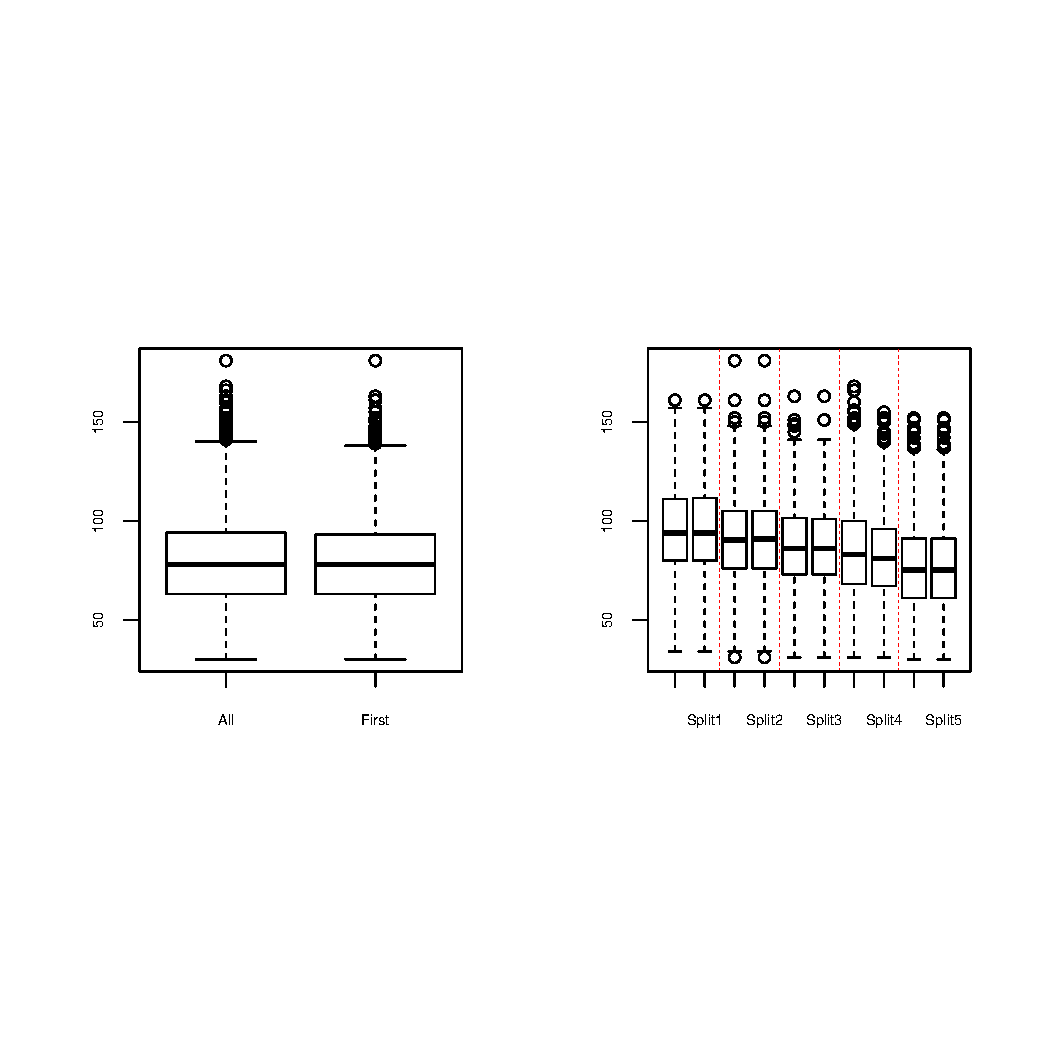
\includegraphics[width=0.8\textwidth, trim=2cm 5cm 2cm 5cm]{all_first.eps}
\caption{PANSS data. Boxplots for the entire set of data, for the subject from the first pattern only, and for various split samples. } \label{fig_all_first}
\end{figure}

To examine the choice of an AR(1) covariance structure, Table~\ref{fig_model_comp} shows three model selection criteria  to compare different error covariance structures. Changing from independence structure ($R=\sigma^2 I$) to compound-symmetry ($R=\sigma^2 I$) the criteria decrease with a large amount, and the same when changing to AR(1). The step to an unstructured covariance does not make a big difference (considering that the unstructured covariance would has $21$ parameters to estimate compared to $2$ parameters in the AR(1) model). Therefore, AR(1) seems to be a good choice.

\begin{table}[t]
\centering
\caption[PANSS data. Comparing different error covariance structures using three model comparison criteria for without trial model]{PANSS data. Comparing different error covariance structures using three model comparison criteria for model (\ref{model_no_trial}) (residual log-likelihood value; AIC; BIC). Three $R$ structures: Ind. : independence structure ($R=\sigma^2 I$), CS: compound-symmetry structure ($R= \sigma^2 I +dJ $), AR(1): AR(1) structure ($R_{ij}=\sigma^2 \rho^{|i-j|}$), UN: unstructured ($R_{ij}=\sigma^2_{ij}$).} \label{fig_model_comp}

\begin{tabular}{lccc}
\hline
\hline
Model&-2 Res.log.lik.&AIC&BIC\\
\hline
Unstructured  &80005.1&80047.1&80164.1\\
AR(1)         &80522.6&80526.6&80537.8\\
Compound symm.&82683.1&82687.1&82698.3\\
Independence  &89546.1&89548.1&89553.7\\
\hline\hline
\end{tabular}
\end{table}

The $95\%$ confidence intervals, accompanying (\ref{model_no_trial}), are presented in Figure~\ref{fig_without_trial}. In order to give more insight in these results, Figure~\ref{fig_without_trial_split} shows the $95\%$ confidence interval in each split, comparing with the full sample splits (the horizontal dashed line in the figure).

The $95\%$ confidence intervals, accompanying (\ref{model_trial}), are presented in Figure~\ref{fig_with_trial}. Figure~\ref{fig_with_trial_split} shows the $95\%$ confidence intervals for the parameter estimates in each split comparing with the full sample estimate (the horizontal dashed-like in the figure.)


\begin{figure}[ht]
\centering
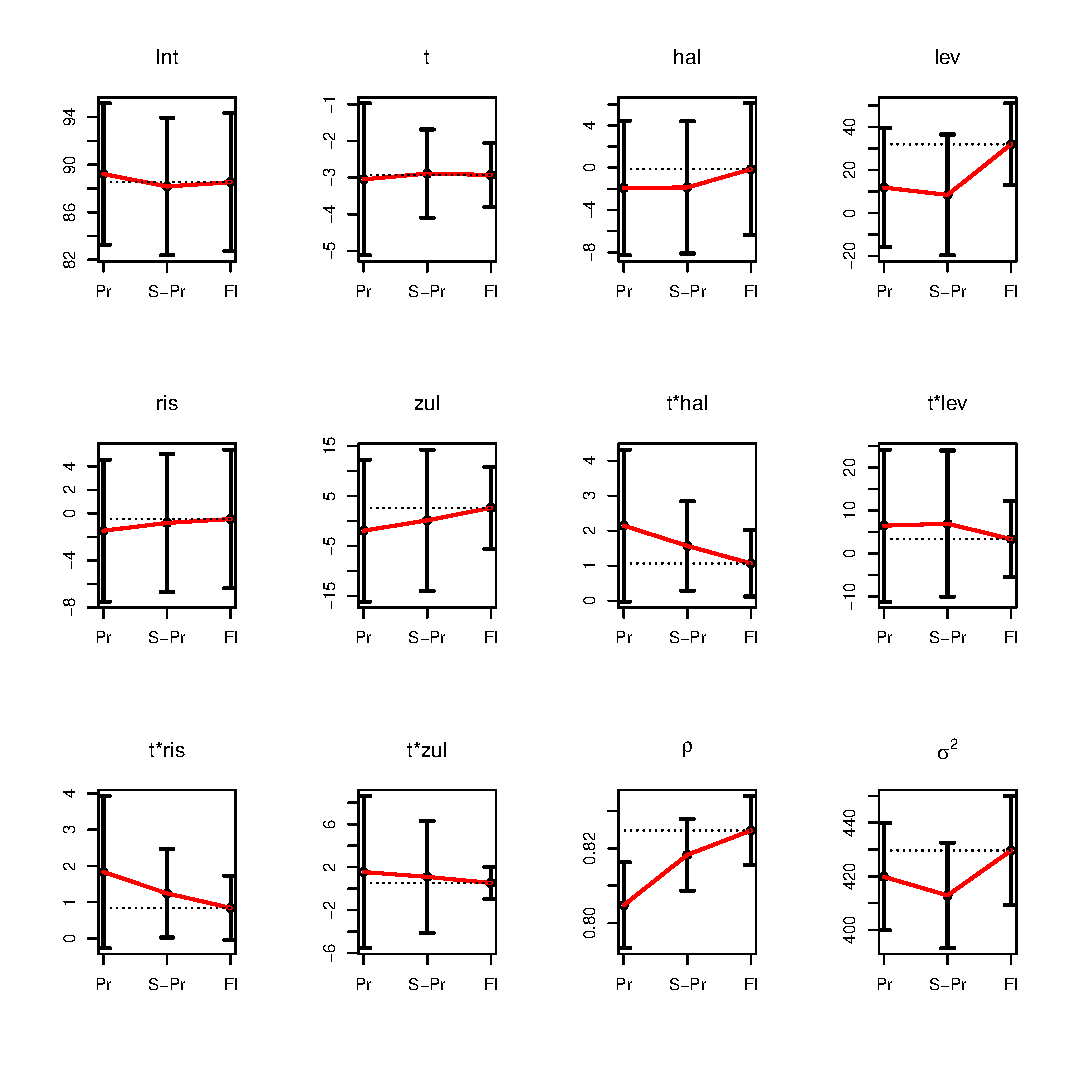
\includegraphics[width=\textwidth]{without_trial.eps}
\caption[PANSS data. $95\%$ confidence intervals for fixed effects and variance components estimates and the standard deviations of these estimates using sample splitting, combined with proportional and size-proportional weights, and full likelihood (without trial model)]{PANSS data. $95\%$ confidence intervals for fixed effects and variance components estimates and the standard deviations of these estimates using sample splitting, combined with proportional (Pr - first) and size-proportional (S-Pr - second) weights, and full likelihood (Fl - third). The dashed horizontal line shows the full likelihood estimate. The model used in here is without trial effect (\ref{model_no_trial}).} \label{fig_without_trial}
\end{figure}

\begin{figure}[ht]
\centering
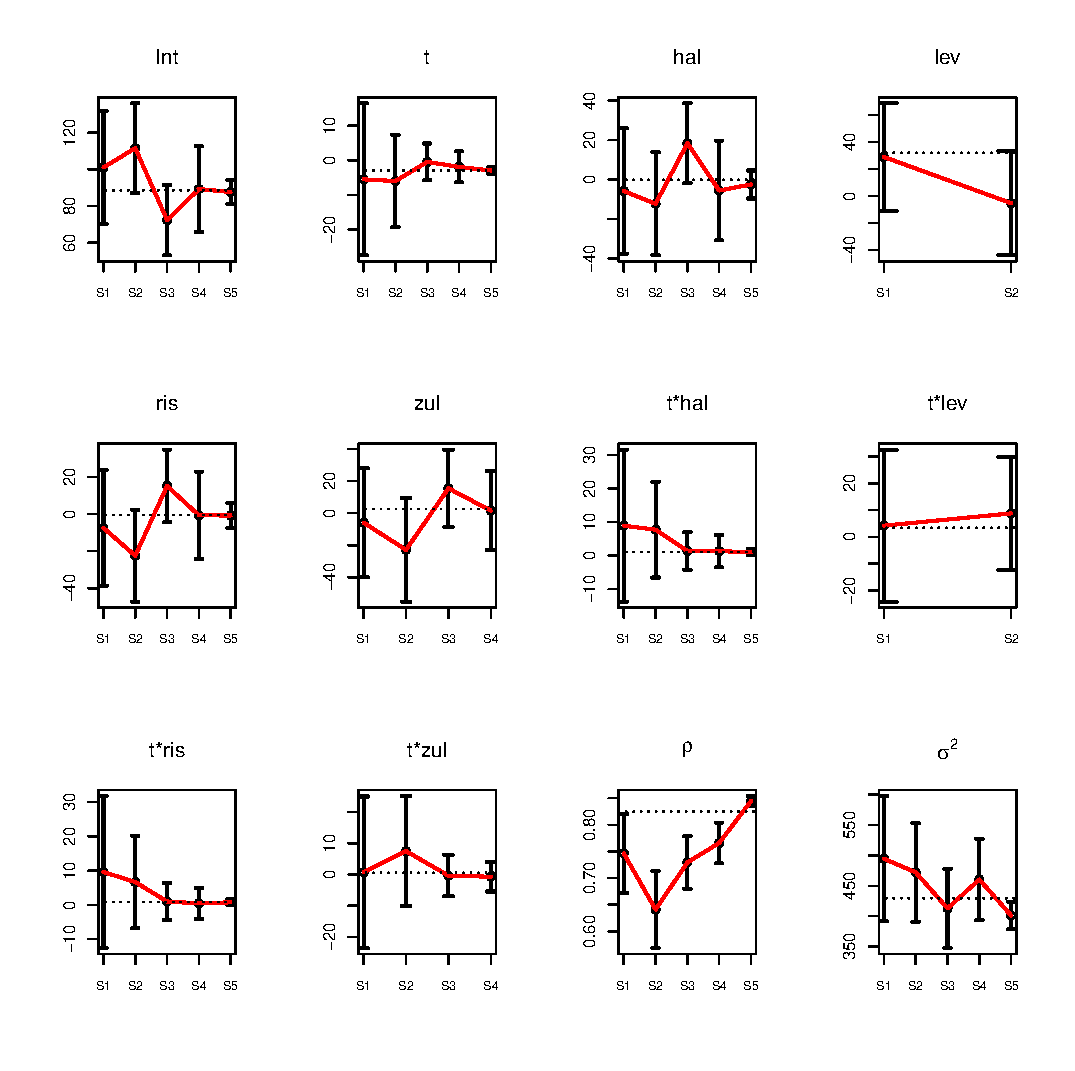
\includegraphics[width=\textwidth]{without_trial_split_by_split.eps}
\caption[PANSS data. $95\%$ confidence intervals for fixed effects and variance components estimates and the standard deviations of these estimates within each split (without trial model)]{PANSS data. $95\%$ confidence intervals for fixed effects and variance components estimates and the standard deviations of these estimates within each split. The dashed horizontal line shows the full likelihood estimate. The model used in here is without trial effect (\ref{model_trial}).} \label{fig_without_trial_split}
\end{figure}

\begin{figure}[ht]
\centering
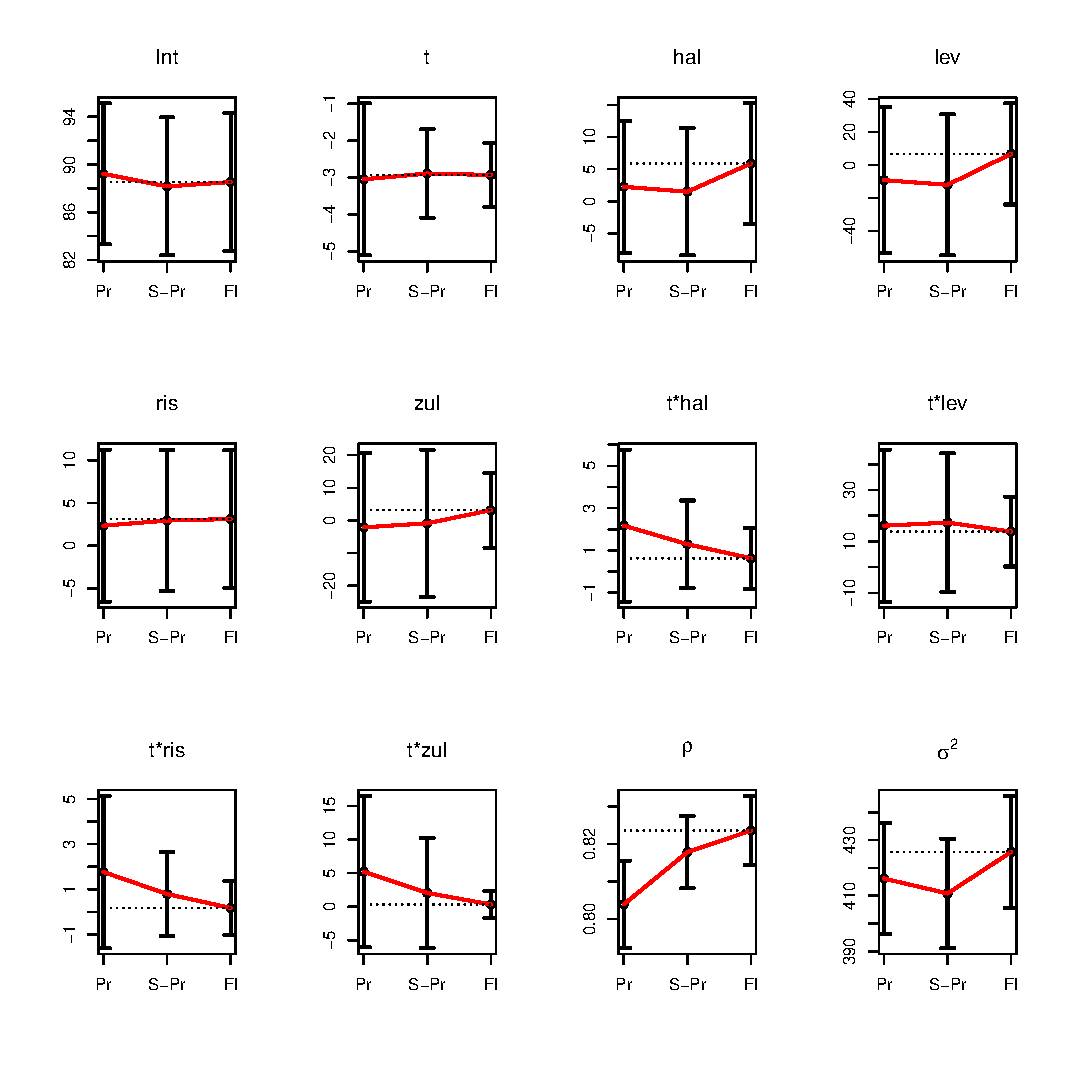
\includegraphics[width=\textwidth]{with_trial.eps}
\caption[PANSS data. $95\%$ confidence intervals for fixed effects and variance components estimates and the standard deviations of these estimates using sample splitting, combined with proportional and size-proportional weights, and full likelihood (with trial model)]{PANSS data. $95\%$ confidence intervals for fixed effects and variance components estimates and the standard deviations of these estimates using sample splitting, combined with proportional (Pr - first) and size-proportional (S-Pr - second) weights, and full likelihood (Fl - third). The dashed horizontal line shows the full likelihood estimate. The model used in here is with trial effect (\ref{model_trial}).} \label{fig_with_trial}
\end{figure}


\begin{figure}[ht]
\centering
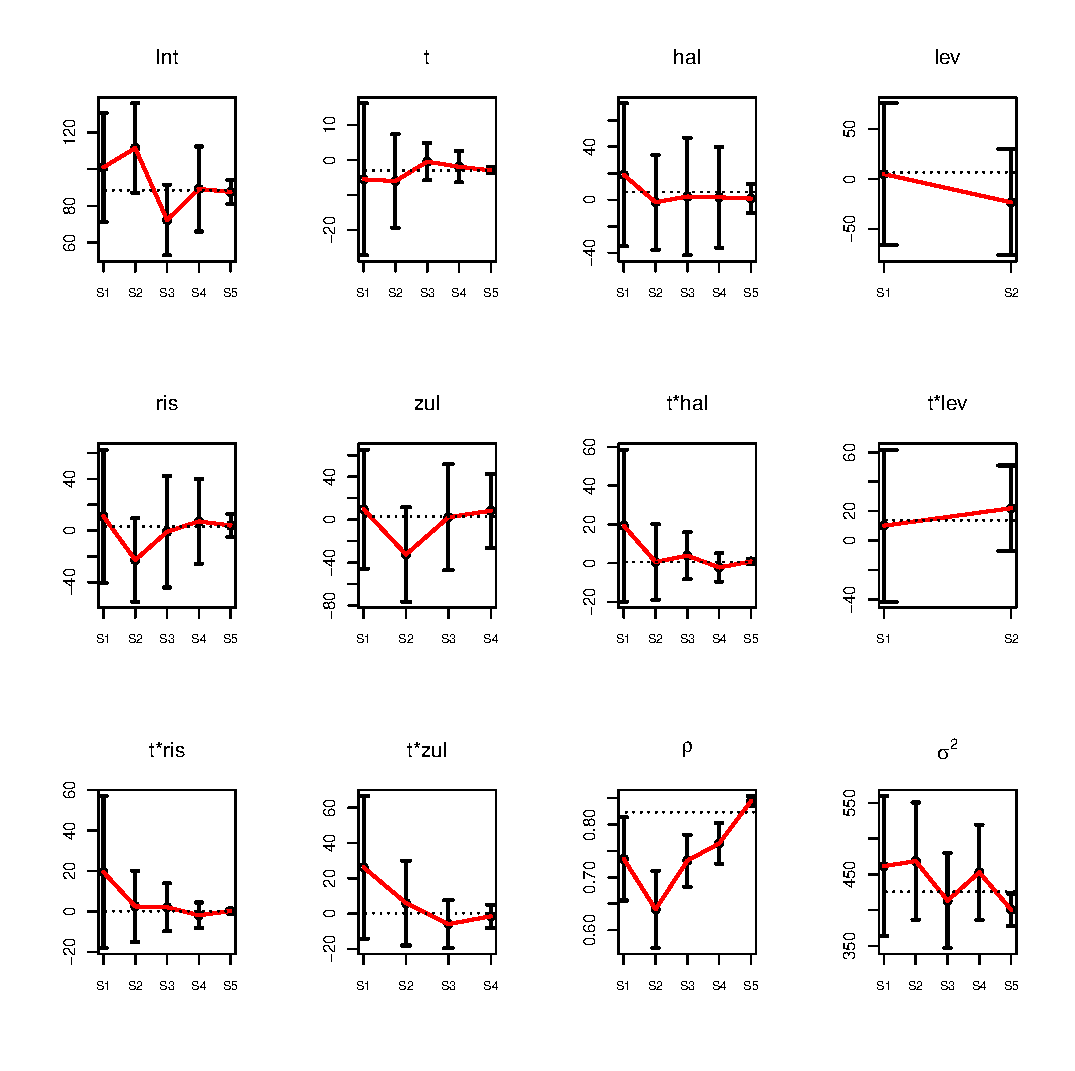
\includegraphics[width=\textwidth]{with_trial_split_by_split.eps}
\caption[PANSS data. $95\%$ confidence intervals for fixed effects and variance components estimates and the standard deviations of these estimates within each split (with trial model)]{PANSS data. $95\%$ confidence intervals for fixed effects and variance components estimates and the standard deviations of these estimates within each split. The dashed horizontal line shows the full likelihood estimate. The model used in here is with trial effect (\ref{model_trial}).} \label{fig_with_trial_split}
\end{figure}



\setcounter{equation}{0}
\section{Fieller's method and delta method}
\label{app1}

Here, the Fieller's method to construct a confidence interval for (\ref{nf_var_min_cs}) as well as the Delta method  are discussed. The ratio which we require a confidence interval for is:
$$n_f=\frac{\hat{\sigma^2}}{\widehat{\tau} \varepsilon}.$$
Suppose $n_1$ is a small-feasible sub-sampling size chosen to estimate the parameters in the model (e.g., $n_1=5$). From \cite{Iddi2011}, one finds:



\begin{multline}
%\label{cov_sigma2_tau}
\mathrm{Var}  \left(
\begin{array}{c}
\widehat{\sigma^2}\\
\widehat{\tau\varepsilon}
\end{array} \right) =  \\ \frac{2 \sigma^4}{Nn_1(n_1-1)}  \left(
\begin{array}{cc}
n_1 & -\varepsilon \\
-\varepsilon & \varepsilon^2\frac{\sigma^4 + 2(n_1-1) \tau \sigma^2 + n_1 (n_1-1) \tau^2}{\sigma^4}
\end{array} \right) \\ = \left(
\begin{array}{cc}
s_{11} &  s_{12} \\ s_{12} & s_{22}
\end{array} \right).
\end{multline}

The Fieller's confidence interval for (\ref{nf_var_min_cs}) can be calculated following these steps.
\begin{equation}
\begin{aligned}
C_1^2 =&\frac{s_{11}}{\widehat{\sigma^2}^2}, \\
C_2^2=& \frac{s_{22}}{\left(\varepsilon\widehat{\tau}\right)^2},\\
r= & \frac{s_{12}}{\sqrt{s_{11} s_{22}}},\\
A= &C_1^2 + C_2^2 - 2r C_1C_2,\\
B=& t^2 C_1^2 C_2^2 (1-r^2),\\
L=& \frac{\widehat{\sigma^2}}{\varepsilon\widehat{\tau}} \frac{1-z_{\alpha/2}^2 r C_1C_2 - z_{\alpha/2}\sqrt{A-B}}{1-z_{\alpha/2}^2C_2^2},\\
U=& \frac{\widehat{\sigma^2}}{\varepsilon\widehat{\tau}} \frac{1-z_{\alpha/2}^2 r C_1C_2 + z_{\alpha/2}\sqrt{A-B}}{1-z_{\alpha/2}^2C_2^2}.
\end{aligned}
\end{equation}
One may take $n_f=\max\{L,U\}$. Of course, in case were $z_{\alpha/2}^2 C_2^2 <1$, there would be no finite interval. As it was mentioned, one may also use the Delta method as follows:
\begin{equation}
\label{var_delta_method}
\mathrm{Var}(\frac{\widehat{\sigma^2}}{\varepsilon \widehat{\tau}}) \approx \frac{1}{\varepsilon^2 \widehat{\tau}^2} \left( s_{11} - 2 \frac{\sigma^2}{\tau} s_{12} + \frac{\sigma^4}{\tau^2} s_{22} \right).
\end{equation}
\setcounter{equation}{0}
\section[Random vertical data splitting for CS]{Random vertical data splitting for compound-symmetry structure}
\label{app2}
Assume a single cluster of size $N$ with multivariate normal distribution and compound-symmetry structure for its covariance matrix, see Section~\ref{sec_CS_effect}. Suppose we take $M_0$ sub-samples of size $n_0$ from this cluster. Following \cite{hoffman2001}, the parameter $\mu$ should be estimated within each sub-sample, $\widehat{\mu}^{(m)}$ ($m=1,\ldots,M_0$) and then the overall estimate can be obtained by averaging these estimates. Furthermore, one needs the within and between sub-samples variabilities to compute the overall variability, see (\ref{mo_cov}).

Within each sub-sample the variance of $\widehat{\mu}^{(m)}$ can be computed using the variance formula for a mean estimator in CS-multivariate normal \cite{Iddi2011} :
\begin{equation}
\label{within}
S_W= \frac{\sigma^2}{n_0} \left[ 1+ (n_0-1) \rho \right ].
\end{equation}
Estimating the between variability requires computing $\mathrm{E}\left\{ (\widehat{\mu}^{(m)} - \bar{\mu})^2 \right\}$, where $\bar{\mu}$ is the average of $\widehat{\mu}^{(m)}$'s ($m=1,\ldots,M_0$). Set $S_m$ as the index of members of sub-sample $m$ and $S_{m'}$ the rest of the sample, then,
\begin{equation*}
\widehat{\mu}^{(m)} - \bar{\mu} = \frac{1}{n_0}\left\{(1-\frac{1}{M_0})\sum_{i\in S_m} y_i - \frac{1}{M_0} \sum_{m=1}^ {M_0} \sum_{i\in S_{m'}} y_i \right\}.
\end{equation*}
Therefore,
\begin{equation}
\label{T1_T4}
\mathrm{E}\left\{(\widehat{\mu}^{(m)} - \bar{\mu})^2 \right\} = \frac{1}{n_0} \left( T_1 + T_2 + T_3+ T_4\right),
\end{equation}
where,
\begin{equation}
\label{eq_T1_T4}
\begin{cases}
T_1= \left( 1- \frac{1}{M_0} \right) \mathrm{E} \left [ \sum_{i\in S_m} y_i \right]^2\\
T_2= \frac{1}{M_0^2} (M_0-1) \mathrm{E} \left[ \sum_{i \in S_m} y_i \right]^2\\
T_3=  -2 \left(1-\frac{1}{M_0} \right) \frac{1}{M_0} (M_0-1) \mathrm{E} \left\{ \left(\sum_{i\in S_{m'}} y_i \right) \left( \sum_{i'\in S_{m'}} y_{i'} \right) \right\} \\
T_4= 2 \frac{1}{M_0} \frac{(M_0-1) (M_0-2)}{2} \mathrm{E} \left\{ \left(\sum_{i \in S_m} y_i \right) \left(\sum_{i'\in S_{m'}} y_{i'} \right) \right\}.
\end{cases}
\end{equation}
From (\ref{eq_T1_T4}) one may find,
\begin{equation}
\label{sum_T}
\begin{cases}
T_1+ T_2 = \frac{M_0-1}{M_0} n_0 \sigma^2 \left [1+ (n_0-1) \rho \right]\\
T_3 + T_4= - \frac{M_0-1}{M_0} \frac{\sigma^2 n_0^2}{N} \left[ 1+ (N_1) \rho \right].
\end{cases}
\end{equation}
Therefore, the between variability can be computed as follows,
\begin{multline}
\label{between}
S_B=\mathrm{E} \left\{ (\widehat{\mu}^{(m)} - \bar{\mu} )^2 \right\} = \\ \frac{M_0-1}{M_0} \left[\frac{1+(n_0-1)\rho}{n_0} - \frac{1+(N_1)\rho}{N} \right].
\end{multline}
Using (\ref{within}) and (\ref{between}), the total variability can be computed as follows,
\begin{equation}
\label{total_variability}
S_T= \frac{1}{M_0} \sigma^2 \frac{1+ (n_0-1) \rho }{n_0} + \frac{M_0-1}{M_0} \sigma^2 \frac{1+ (N-1) \rho}{N}
\end{equation}
Comparing the variance in (\ref{total_variability}) with the variance when estimating $\mu$ using the full sample would give,
\begin{equation}
\label{ARE}
\mathrm{ARE} = \frac{M_0-1}{M_0} + \frac{1}{M_0} \frac{N}{n_0} \frac{1+(n_0-1) \rho}{1+ (N-1) \rho}
\end{equation}
For example, if sub-sampling is done only once ($M_0=1$), then,
\begin{equation}
\label{ARE_M1}
\mathrm{ARE} = \frac{N}{n_0} \frac{1+(n_0-1) \rho}{1+(N-1) \rho},
\end{equation}
The same calculation is possible for $M_0=2$,
\begin{equation}
\label{are_M02}
\mathrm{ARE}= \frac{1}{2} + \frac{1}{2} \frac{N}{n_0} \frac{1+(n_0-1) \rho}{1+ (N-1) \rho}.
\end{equation}
By considering the desired ARE as $1+\epsilon$, one may find $n_0$.


\setcounter{equation}{0}
\section{Combination rule for $p$-values for MI}
\label{app_mi}

The Kruskal-Wallis test statistic asymptotically follows a $\chi^2$ distribution. Therefore, in order to find the combined $p$-value, we may follow the procedure proposed by \cite{li1991}. More details can be found in \cite{rubin2004} and \cite{enders2010}. The combination is done using {\tt{micombine.chisquare}} in package {\tt{miceadds}} in \textsf{R}, \cite{miceadds}.

\begin{itemize}
	\item \textbf{Averaging.} Compute the test statistic for each imputed data and take their average: $\overline{\chi^2} = \frac{1}{M} \sum_{m=1}^M \chi^2_m$.
	\item \textbf{Relative variance increase.} $r=\left(1+\frac{1}{M} \right) \frac{\sum_{m=1}^M (\sqrt{\chi^2_m} - \sqrt{\overline{\chi^2}})^2}{M-1}$
	\item \textbf{Test statistic.} $D=\frac{\frac{\overline{\chi^2}}{\kappa} - \frac{M+1}{M-1}r}{1+r}$, where $\kappa$ is the degrees-of-freedom of the $\chi^2_m$. For a $\chi^2$-test of independence, it is $(k_1-1)(k_2-1)$ where $k_1$ and $k_2$ are the number of levels of two categorical variables. Take five diagnosis groups and variable \textsf{Eye} with two levels, then $\kappa=(5-1)(2-1)=4$. For the Kruskal-Wallis test, $\kappa$ is the number of groups minus 1. So, when comparing values of a continuous variable among three types of diagnosis, $\kappa=2$. When this comparison is done for all five types, $\kappa=4$. 
	\item \textbf{Computing $p$-value.} $p$-value$=P(F_{\kappa,\nu} > D)$, where $F$ is the $F$-distribution and $\nu=\kappa^{-3/M} (M-1) \left(1+\frac{1}{r}\right)^2$
\end{itemize}
\newpage~
\setcounter{equation}{0}
\setcounter{page}{355}
\section{The surrogate model}
\label{sec_surrogate_model}
The model takes the form:
\begin{equation}
\label{surrogatemodel}
\left\{
\begin{array}{l}
S_{ij}=\mu_S + m_{S_i} + (\alpha + a_i) Z_{ij} + \varepsilon_{S_{ij}},\\
T_{ij}= \mu_T + m_{T_i} + (\beta + b_i) Z_{ij} + \varepsilon_{T_{ij}},
\end{array} \right.
\end{equation}
where $S_{ij}$ and $T_{ij}$ are the surrogate and true endpoints, and $Z_{ij}$ is the treatment indicator (1 for active; 0 for placebo), respectively. Index $i$ refers to the trial and $j$ to the subject. Further, $\mu_{S}$ and $\mu_{T}$ are fixed intercepts and $m_{S_i}$ and $m_{T_i}$ are  random intercepts, for surrogate and true endpoint, respectively. The fixed treatment effects are $\alpha$ (for $S$) and $\beta$ (for $T$), and the centre-specific treatment effects are $a_i$ (for $S$) and $b_i$ (for $T$). 
Random intercepts and slopes are assumed to follow
$(m_{S_i}, m_{T_i}, a_i, b_i)'\sim N(0,D)$,
where 
\begin{equation}
\label{D}
D = \left(
\begin{array}{cccc}
d_{SS} & & &\\
d_{ST} & d_{TT} & &\\
d_{Sa} & d_{Ta} & d_{aa} &\\
d_{Sb} & d_{Tb} & d_{ab} & d_{bb}
\end{array} \right).
\end{equation}
Furthermore, for the error terms,
\begin{equation}
\label{surrogateSigma}
\left(\begin{array}{c}
\varepsilon_{S_{ij}}\\
\varepsilon_{T_{ij}}
\end{array} \right)
\sim N(0,\Sigma),\; \Sigma = \left(
\begin{array}{cc}
\sigma_{SS} & \\
\sigma_{ST} & \sigma_{TT}
\end{array} \right).
\end{equation}
The parameters of interest for the surrogate evaluation are trial- and individual-level coefficients of determination, $R^2_{\mbox{\tiny trial}}$ and $R^2_{\mbox{\tiny indiv}}$, respectively:
\begin{equation}
\label{R2}
\begin{gathered}
R^2_{\mbox{\tiny trial}} = \frac{1}{d_{ab}}
\left(
\begin{array}{c}
d_{Sb}  \\
d_{ab}
\end{array} \right)^{\prime} 
\left(
\begin{array}{cc}
d_{SS} & d_{Sa}\\
d_{Sa} & d_{aa}
\end{array} \right)^{-1}
\left(
\begin{array}{c}
d_{Sb}  \\
d_{ab}
\end{array} \right),\\ R^2_{\mbox{\tiny indiv}}=\frac{\sigma_{ST}^2}{\sigma_{SS} \sigma_{TT}}.
\end{gathered}
\end{equation}



\bibliography{thesis_leuven_bib}{}
\bibliographystyle{abbrvnat}


\end{document}












